\documentclass[11pt]{article}

\usepackage[margin=1in]{geometry}
\usepackage{amsmath,amssymb,amsthm,mathtools}
\usepackage{listings}
\usepackage{microtype}
\usepackage{graphicx}
\usepackage{float}
\usepackage{longtable}
\usepackage{tikz}
\usepackage[hidelinks]{hyperref}
\hypersetup{linktoc=all}
\setcounter{tocdepth}{2}
\makeatletter
\renewcommand{\l@subsection}{\@dottedtocline{2}{1.5em}{3.4em}}
\makeatother
\usetikzlibrary{arrows.meta,calc,positioning}

\newtheorem{theorem}{Theorem}
\newtheorem{lemma}[theorem]{Lemma}
\newtheorem{definition}[theorem]{Definition}

\title{CJR Collections: Verified Data Structures and Algorithms}
\author{Dan R. Ghica}
\date{\today}

\lstdefinestyle{coq}{
  basicstyle=\ttfamily\small,
  columns=fullflexible,
  keepspaces=true,
  showstringspaces=false,
  breaklines=true,
  frame=single,
  framerule=0.3pt,
  xleftmargin=0.4em,
  xrightmargin=0.4em,
  aboveskip=0.8em,
  belowskip=0.8em,
  literate={Σ}{{$\Sigma$}}1
           {↦ₛ}{{$\mapsto_s$}}2
           {↦ₒ}{{$\mapsto_o$}}2
           {λ}{{$\lambda$}}1
           {↦ₒ}{{$\mapsto_o$}}2
           {→}{{$\rightarrow$}}1
           {∀}{{$\forall$}}1
           {∃}{{$\exists$}}1
           {∗}{{$*$}}1
           {⌜}{{$\ulcorner$}}1
           {⌝}{{$\urcorner$}}1
           {≤}{{$\leq$}}1
           {∧}{{$\land$}}1
           {∨}{{$\lor$}}1
           {∈}{{$\in$}}1
           {⊢}{{$\vdash$}}1
           {≠}{{$\neq$}}1
           {∉}{{$\notin$}}1
           {∅}{{$\emptyset$}}1
}
\lstset{style=coq}

\newcommand{\cjr}{CJR}
\newcommand{\sem}[1]{[\![#1]\!]}
\newcommand{\step}{\longrightarrow}
\newcommand{\steps}{\longrightarrow^{*}}
\newcommand{\Stuck}{\mathsf{stuck}}
\newcommand{\WF}{\mathsf{wf}}
\newcommand{\dom}{\operatorname{dom}}
\newcommand{\lookup}[2]{#1(#2)}
\newcommand{\None}{\mathsf{None}}
\newcommand{\Some}{\mathsf{Some}}
\newcommand{\Unit}{\mathsf{()}}
\newcommand{\True}{\mathsf{true}}
\newcommand{\False}{\mathsf{false}}
\newcommand{\NULL}{\mathsf{null}}
\newcommand{\pts}{\mathrel{\mapsto}}
\newcommand{\ptss}{\mathrel{\mapsto_{s}}}
\newcommand{\ptsr}{\mathrel{\mapsto_{r}}}
\newcommand{\ptsb}{\mathrel{\mapsto_{b}}}
\newcommand{\ptso}{\mathrel{\mapsto_{o}}}
\newcommand{\sep}{\mathbin{*}}
\newcommand{\bigsep}{\mathop{\scalebox{1.4}{$\ast$}}}
\newcommand{\wand}{\mathbin{-\!\!*}}
\newcommand{\later}{\mathop{\triangleright}}
\newcommand{\Wpre}{\mathsf{wp}}
\newcommand{\GWpre}{\mathsf{gwp}}
\newcommand{\pure}[1]{\ulcorner #1 \urcorner}

\begin{document}
\maketitle
\tableofcontents
\clearpage
\section{Setup and proof boundary}
This repository uses CJR Core and the Coq 8.20.1, stdpp 1.12.0, Iris 4.4.0 toolchain. Read the local README for pinned dependency paths. The CJR logic reasons about its operational model; printing, native compilation, machine integer overflow, and external adapters require separate care. Proofs were not revalidated during this migration.
\section{A linked list}

The file \texttt{example/list/rocq/list.v} is a self-contained implementation of a singly linked list, together with the equations that say the implementation really is a list.
It is larger than the earlier examples because the specification is not a single pure result: it is a predicate on the object heap, and the programs are functions that allocate and read nodes.
This existing list stores integers. The generic \texttt{Pair} and
\texttt{Box} examples do not automatically make it a \texttt{List<T>}:
that would require a parameterised node declaration and a list
representation predicate carrying an element predicate at every node.

\subsection{Why a node is an object with a boolean tag}

A textbook list cell is a pair of a head and a pointer to the rest, and the empty list is the null pointer.
\cjr{} has null, and loading through null is stuck, which is the right machine behaviour.
What it does not have is an equality test on pointers or on object references.
\texttt{EqOp} compares integers only.
A program therefore cannot branch on ``is this pointer null?''.

The sticking point is resolved by using a non-\texttt{open} class with three fields, and a boolean the language can already branch on.

\begin{lstlisting}
Definition nil_body : expr :=
  Let (Some "n")
    (New [LitV (LitBool false); LitV (LitInt 0); LitV LitUnit] [])
    (Seq (FieldStore (Var "n") 2 (Var "n")) (Var "n")).

Definition cons_body : expr :=
  Let (Some "x") (StructLoad (Var "a") 0)
    (Let (Some "xs") (StructLoad (Var "a") 1)
      (New [] [Val (LitV (LitBool true)); Var "x"; Var "xs"])).
\end{lstlisting}

Field \(0\) is the tag: \(\False\) means empty, \(\True\) means cons.
Field \(1\) is the head integer, which is \(0\) and unused when the tag is false.
Field \(2\) is the tail.
On an empty node it is that same node; on a cons node it is the value that represents the rest of the list, itself either an empty node or another cons node.
The allocation writes unit into the field and then stores the new object there before \texttt{nil} returns.
The points-to fact owns the field.
The value in the field is a pointer to the object, so the fact does not own the object a second time, and the predicate does not unfold.
Objects are not freed, so a cons cell stays in the heap after its tail has been read.
That matches the language: there is a \texttt{new} rule and no rule that deletes an object.

In Cangjie the operations are ordinary functions.
Core application takes one argument, so \texttt{cons(x, xs)} lowers to a call on the struct of those two arguments.
The other functions take the node.

\lstinputlisting{example/list/extracted/list.cj}

A Cangjie constructor cannot receive the object it is building, so the printed class takes an optional tail and stores it in a raw field.
Unit, the placeholder written by the allocation, is printed as \texttt{None}.
The property \texttt{next} reads that raw field back as a \texttt{Node}: the stored node when it is present, and the node itself when it is empty.
After \texttt{nil} returns, the raw tail has been set to the node.
\texttt{empty} does not read \texttt{next}.
The functions above are the Cangjie surface; \texttt{cons} of two arguments lowers to the unary core call on the struct \(\langle x, xs\rangle\).

\texttt{empty} returns the negation of the tag.
An empty node is empty; a cons node is not.
The conditional is the only test.
It does not inspect the tail pointer.

\subsection{The representation predicate}

On paper, a mathematical list \(xs\) is related to a value \(p\) by \(\mathsf{isList}(xs, p)\).

\begin{definition}[List representation]
\(\mathsf{isList}([], p)\) holds when \(p = \mathsf{obj}(o)\) and
\[
o \ptso[0] \False
\sep
o \ptso[1] 0
\sep
o \ptso[2] \mathsf{obj}(o).
\]
\(\mathsf{isList}(x :: xs, p)\) holds when \(p = \mathsf{obj}(o)\) and there is a tail value \(q\) with
\[
o \ptso[0] \True
\sep
o \ptso[1] x
\sep
o \ptso[2] q
\sep
\mathsf{isList}(xs, q).
\]
\end{definition}

The Coq predicate is the same recursion, as a separation-logic assertion.

\begin{lstlisting}
Fixpoint is_list (xs : list Z) (p : val) : iProp S :=
  match xs with
  | [] => exists o, pure (p = LitV (LitObj o)) *
      ObjId o |->o[0] LitV (LitBool false) *
      ObjId o |->o[1] LitV (LitInt 0) *
      ObjId o |->o[2] LitV (LitObj o)
  | x :: xs' => exists o nxt, pure (p = LitV (LitObj o)) *
      ObjId o |->o[0] LitV (LitBool true) *
      ObjId o |->o[1] LitV (LitInt x) *
      ObjId o |->o[2] nxt *
      is_list xs' nxt
  end.
\end{lstlisting}

\textit{What the separating conjunction is doing.}
The three fields of one node are three separate facts, so a proof may load the tag and still own the head and the tail.
The recursive fact \(\mathsf{isList}(xs, q)\) owns every node of the tail and nothing of the cons cell.
Those two regions are disjoint.
That is why ``the tail is the original list'' can be stated by returning the original pointer together with \(\mathsf{isList}(xs, p)\), while the cons cell's own three fields sit beside it rather than inside it.

A value that is not an object reference does not satisfy \(\mathsf{isList}\).
The lemma \texttt{is\_list\_obj} records the useful direction: if the predicate holds, the value is \(\mathsf{obj}(o)\) for some \(o\).
The proofs rewrite with that equality before they substitute, so an abstract pointer is a literal object reference by the time it is placed in a struct.
Substitution then computes.

\subsection{What each operation establishes}

\paragraph{Empty list.}
\[
\Wpre\,\mathsf{nil}()\,\{\,v.\; \mathsf{isList}([], v)\,\}.
\]
\texttt{wp\_new} returns ownership of the three initial fields. The tail initially holds unit.
\texttt{wp\_field\_store} then writes the new object into that field, which is the empty clause.
Nothing else is allocated.
This is \texttt{nil\_spec}.

\paragraph{Cons.}
\[
\mathsf{isList}(xs, p)
\vdash
\Wpre\,\mathsf{cons}\,\langle x, p\rangle
\,\Bigl\{\,v.\;
  \exists o.\;
  v = \mathsf{obj}(o)
  \sep
  o \ptso[0] \True
  \sep
  o \ptso[1] x
  \sep
  o \ptso[2] p
  \sep
  \mathsf{isList}(xs, p)
\,\Bigr\}.
\]
The argument struct is unboxed.
\texttt{wp\_struct\_load} copies \(x\) and then \(p\) out of it; those loads do not touch the heap.
The body then allocates one object.
The third field is the original pointer \(p\), not a copy of the tail's nodes.
The fact \(\mathsf{isList}(xs, p)\) is framed across allocation: \texttt{wp\_new} does not ask for it, so it cannot be changed.
The postcondition is the unfolding of \(\mathsf{isList}(x :: xs, v)\) with the tail pointer pinned to the pointer that was passed in.
Pinning it is what makes the later inverse law an equality of values, not only an equality of mathematical lists up to some existential.
This is \texttt{cons\_spec}.

\paragraph{Head.}
\[
\mathsf{isList}(x :: xs, p)
\vdash
\Wpre\,\mathsf{head}\,p
\,\{\,v.\; \pure{v = x} \sep \mathsf{isList}(x :: xs, p)\,\}.
\]
The proof opens the cons clause, loads field \(1\), and puts the same facts back together.
The list predicate after the call is the list predicate before the call.
Head is a pure observation.
This is \texttt{head\_spec}.

\paragraph{Tail.}
\[
\begin{aligned}
&\mathsf{isList}(x :: xs, p) \vdash {}\\
&\quad\Wpre\,\mathsf{tail}\,p
\,\Bigl\{\,v.\;
  \mathsf{isList}(xs, v)
  \sep
  \exists o.\;
  p = \mathsf{obj}(o)
  \sep
  o \ptso[0] \True
  \sep
  o \ptso[1] x
  \sep
  o \ptso[2] v
\,\Bigr\}.
\end{aligned}
\]
Loading field \(2\) returns the tail pointer and gives the points-to fact back.
The recursive clause of \(\mathsf{isList}\) already owned \(\mathsf{isList}(xs, v)\) separately from the cons cell, so the postcondition splits the list into the cell that was examined and the list that remains.
It does not duplicate nodes.
This is \texttt{tail\_spec}.

\paragraph{Emptiness.}
\[
\begin{aligned}
\mathsf{isList}([], p)
  &\vdash
  \Wpre\,\mathsf{empty}\,p
  \,\{\,v.\; \pure{v = \True} \sep \mathsf{isList}([], p)\,\},\\
\mathsf{isList}(x :: xs, p)
  &\vdash
  \Wpre\,\mathsf{empty}\,p
  \,\{\,v.\; \pure{v = \False} \sep \mathsf{isList}(x :: xs, p)\,\}.
\end{aligned}
\]
Both proofs load the tag and take one branch of \texttt{if}.
The other branch is dead in that specification: a proof of the empty law never has to show anything about the cons branch, and conversely.
The predicate is restored, so emptiness is an observation rather than a destructive read.
These are \texttt{empty\_nil} and \texttt{empty\_cons}.

\subsection{Adding an element and removing it}

The program that the inverse law talks about is the composition of the two functions, not a fused implementation.

\begin{lstlisting}
Definition cons_then_tail (x : Z) (p : val) : expr :=
  Let (Some "node") (call_cons x p)
    (App (Rec None (Some "n") tail_body) (Var "node")).
\end{lstlisting}

\begin{theorem}[Cons then tail]
\[
\mathsf{isList}(xs, p)
\vdash
\Wpre\,(\mathsf{tail}\,(\mathsf{cons}\,\langle x, p\rangle))
\,\{\,v.\; \pure{v = p} \sep \mathsf{isList}(xs, v)\,\}.
\]
\end{theorem}

The Coq statement is \texttt{cons\_then\_tail\_spec}.
Read it as an equation of lists.
The value returned by removing the element just added is the original pointer, and that pointer still represents the original mathematical list.

The proof follows the program in order.
\begin{enumerate}
\item \texttt{cons\_spec} allocates the node and frames \(\mathsf{isList}(xs, p)\).
Its postcondition says field \(2\) of the new object is exactly \(p\), and the original list predicate is still owned.
\item The \texttt{let} substitutes that object for \texttt{node}.
\item \texttt{tail} is the function above.
It loads field \(2\).
The load rule returns the value that the points-to fact describes, which is \(p\), and it returns the points-to fact as well.
\item The cons cell's three fields are no longer needed for the equation.
They are discarded.
Iris assertions are affine, so ownership of leftover cells may be dropped.
The object remains allocated in the machine; the specification simply stops mentioning it.
What remains is \(\pure{v = p}\) and \(\mathsf{isList}(xs, p)\).
\end{enumerate}

Two companion readings are already in the lemmas above, and they are the other usual equations.
Head after cons returns \(x\) and still owns \(\mathsf{isList}(x :: xs, \cdot)\).
Emptiness distinguishes \([]\) from \(x :: xs\).
Together they say that the tag, the head field, and the tail field agree with the mathematical constructors, and that reading them does not damage the list those constructors describe.

The next section proves in-place reversal of an arbitrary finite list using this representation.
It opens one cons cell at a time, rewires its tail, and transfers that cell into a separate accumulator.
Append remains outside this development.

\section{In-place list reversal}
\label{sec:list-reversal}

The file \texttt{example/list\_rev/rocq/list\_rev.v} proves the classic iterative
reversal of a singly linked list. This example changes the links of existing
cons cells. It does not allocate replacement cons cells, copy the integers, or
change the tag and head fields. It does allocate one fresh empty sentinel at
entry, because the two list predicates in the loop invariant must own separate
empty nodes. The old sentinel remains allocated when the loop finishes.
The functional theorem describes the reversed contents; the proof also explains
which field changes at each iteration and why that mutation is safe.

\subsection{The representation being reused}

There is one list representation in the development: \texttt{list.is\_list}
from the preceding section. Reversal imports it rather than defining a second
predicate. Its two clauses are
\[
\begin{aligned}
\mathsf{isList}([],p) \equiv {}&
 \exists o.\;\pure{p=\mathsf{obj}(o)}
 \sep o\ptso[0]\False \sep o\ptso[1]0 \sep o\ptso[2]\mathsf{obj}(o),\\
\mathsf{isList}(x::v,p) \equiv {}&
 \exists o,q.\;\pure{p=\mathsf{obj}(o)}
 \sep o\ptso[0]\True \sep o\ptso[1]x \sep o\ptso[2]q
 \sep\mathsf{isList}(v,q).
\end{aligned}
\]
The predicate owns all three fields of each node, including the terminal empty
node. Its separating conjunction makes the recursive tail separate from the
current cons cell. A finite list described this way cannot contain a cycle of
cons cells or repeated ownership of a cons cell. The sentinel's self-link is
allowed because the empty clause owns its three fields directly and does not
recurse through that link.

This ownership is the permission to perform the reversal. Another logical
client cannot simultaneously hold full ownership of the same fields. An
ordinary program variable can still contain an alias to a node: the algorithm
mutates that node, so observations through such an alias change too. The
specification transfers the input list's ownership into ownership of the
returned list; it does not promise that the original head still denotes the
original sequence.

\subsection{The client specification}

The main statement is \texttt{reverse\_spec}:
\[
\mathsf{isList}(xs,p)\vdash
 \Wpre\,\mathsf{reverse}(p)
 \,\{\,r.\;\mathsf{isList}(\mathsf{rev}(xs),r)\,\}.
\]
Here \(xs\) is a mathematical list of integers and \(p\) is a runtime value.
The list predicate connects them. The output predicate establishes both the
order of all values and a well-formed owned list. There is no positive-length
precondition; the empty and singleton cases are included.

The theorem uses Iris's ordinary weakest precondition, hence partial
correctness and safety. It states the postcondition whenever execution returns
and rules out getting stuck under its ownership precondition. The loop proof
uses induction on the unprocessed finite list, which explains why each
iteration consumes one remaining element. This chapter does not claim a
separate total-correctness theorem, exact instruction count, physical pointer
identity theorem, or verified equivalence between the CJR semantics and the
Cangjie compiler. Executable tests complement the checked CJR theorem.

By framing, a separate assertion \(R\) can accompany the input and output:
\(\mathsf{isList}(xs,p)\sep R\) is transformed into
\(\mathsf{isList}(\mathsf{rev}(xs),r)\sep R\). The proof needs none of the
resources in \(R\); a disjoint second list is a concrete example.

\subsection{The iteration definition: \texttt{rev\_step}}

\begin{minipage}{\linewidth}
\lstinputlisting[firstline=61,lastline=65]{example/list_rev/rocq/list_rev.v}
\end{minipage}

The immutable \texttt{let nxt} reads field \(2\) before the program overwrites
it. Without this saved value, the algorithm would lose access to the remaining
input. The field store then changes \texttt{cur.next} to the accumulator.
The assignments make the current node the new accumulator head and advance
\texttt{cur} to the saved tail. Their order matters: assigning \texttt{cur}
first would lose the reference needed for \texttt{acc := cur}.

Only field \(2\) is changed. The current node retains its true tag and its
integer. After the store, that node and the old accumulator describe one new
list with contents \(x::u\). The saved tail describes the remaining suffix
\(v'\). The logical split follows the physical change in links.

\subsection{The loop definition: \texttt{rev\_loop}}

\begin{minipage}{\linewidth}
\lstinputlisting[firstline=67,lastline=68]{example/list_rev/rocq/list_rev.v}
\end{minipage}

The condition loads the current node's tag. True means a cons node and permits
one iteration; false means the empty sentinel and exits. The program does not
use null as the stopping condition. The guard never reads field \(2\) of the
empty node, so its self-link does not cause an extra iteration.

\subsection{The function body: \texttt{rev\_body}}

\begin{minipage}{\linewidth}
\lstinputlisting[firstline=70,lastline=74]{example/list_rev/rocq/list_rev.v}
\end{minipage}

\texttt{call\_nil} allocates and initializes the fresh empty accumulator.
\texttt{VarBind} allocates mutable stack bindings for \texttt{acc} and
\texttt{cur}; \texttt{n} is the immutable function argument. The final expression
reads the accumulator after the loop.

\subsection{The call wrapper: \texttt{call\_reverse}}

\begin{minipage}{\linewidth}
\lstinputlisting[firstline=76,lastline=77]{example/list_rev/rocq/list_rev.v}
\end{minipage}

\texttt{call\_reverse} packages the body as a closure with one immutable
argument \texttt{n}, then applies it to the supplied runtime value. The
wrapper makes the client theorem talk about one complete function call rather
than an open expression with a free argument.

For an input with \(n\) cons cells, the source algorithm traverses those cells
once and uses a constant number of local references. The only new list object
is the empty sentinel. This is the intended linear-time, constant-extra-space
algorithm; no resource-cost theorem is asserted by \texttt{reverse\_spec}.

\subsection{Loading a local: \texttt{sld}}

\begin{minipage}{\linewidth}
\lstinputlisting[firstline=57,lastline=57]{example/list_rev/rocq/list_rev.v}
\end{minipage}

A \texttt{VarBind} replaces reads of a mutable variable with loads from a fresh
stack slot. \texttt{sld z} abbreviates this concrete stack-load expression.
Its argument is the slot's location, not the object reference stored there.
The iteration proof uses the stack points-to fact to obtain that reference
and then separately uses object-field ownership to access the node.

\subsection{Assigning a local: \texttt{sas}}

\begin{minipage}{\linewidth}
\lstinputlisting[firstline=58,lastline=59]{example/list_rev/rocq/list_rev.v}
\end{minipage}

\texttt{sas z e} evaluates the expression \(e\) and writes the resulting value
into stack slot \(z\). It changes the local reference rather than any object
field. This distinction accounts for the three different writes in one
iteration: one object-link write and two local-reference writes.

\subsection{The iteration after substitution: \texttt{rev\_step\_at}}

\begin{minipage}{\linewidth}
\lstinputlisting[firstline=79,lastline=82]{example/list_rev/rocq/list_rev.v}
\end{minipage}

After allocating the accumulator and current bindings at locations
\(l_a,l_c\), this is the iteration that actually executes in the CJR semantics.
It reads the saved tail through \texttt{sld lc}, stores \texttt{sld la} in the
current object's link, and performs the two local assignments using
\texttt{sas}. It exposes the evaluation contexts used in the ownership proof.
It is a proof-facing form of \texttt{rev\_step}, not a second algorithm.

\subsection{The loop after substitution: \texttt{rev\_loop\_at}}

\begin{minipage}{\linewidth}
\lstinputlisting[firstline=84,lastline=85]{example/list_rev/rocq/list_rev.v}
\end{minipage}

The guard loads field \(0\) of the object referenced by the current stack
slot, and the body is the substituted iteration. The accumulator location
appears only in the body. Cangjie is printed from \texttt{rev\_body}, whose
local variables retain their source names; these administrative stack forms
are used to connect that source expression to primitive proof rules.

\subsection{Iteration substitution: statement and proof}

\begin{minipage}{\linewidth}
\lstinputlisting[firstline=87,lastline=91]{example/list_rev/rocq/list_rev.v}
\end{minipage}

This equality connects the named iteration with code operating on two stack
slots. The proof reduces \texttt{subst\_var} structurally through the
expression constructors. \texttt{f\_equal} reduces equality of matching
constructors to equality of their arguments; the remaining equalities are
reflexive. This is an ordinary Coq equality between syntax trees. It assumes
no ownership and executes no command.

\subsection{Loop substitution: statement and proof}

\begin{minipage}{\linewidth}
\lstinputlisting[firstline=93,lastline=98]{example/list_rev/rocq/list_rev.v}
\end{minipage}

This proof unfolds the loop, reduces substitution in the condition, and uses
\texttt{rev\_step\_at\_subst} for its body. Thus it connects the entire named
loop to the loop verified over concrete stack slots. The main function proof
uses the reverse order of the substitutions, which is definitionally the same
for these two distinct variable names.

\subsection{The loop invariant: \texttt{rev\_inv}}

\begin{minipage}{\linewidth}
\lstinputlisting[firstline=100,lastline=106]{example/list_rev/rocq/list_rev.v}
\end{minipage}

The witnesses \(u,v\) are respectively the contents of the accumulator and
the unprocessed suffix. The witnesses \(a,c\) are their runtime references.
The assertion says
\[
\exists u,v,a,c.\;
 \pure{\mathsf{rev}(u)\mathbin{+\mkern-6mu+}v=xs}
 \sep l_a\ptss a \sep l_c\ptss c
 \sep\mathsf{isList}(v,c)\sep\mathsf{isList}(u,a).
\]
The accumulator already has reversed order. Reversing it mathematically
recovers the processed prefix of the original input. Appending the remaining
suffix must recover the entire original list. The stack facts describe the
current values of the two mutable bindings, and the two list predicates give
separate ownership of both chains.

For \(xs=[1,2,3]\), the successive pairs \((u,v)\) are
\(([],[1,2,3])\), \(([1],[2,3])\), \(([2,1],[3])\), and
\(([3,2,1],[])\). For instance,
\(\mathsf{rev}([2,1])\mathbin{+\mkern-6mu+}[3]=[1,2,3]\).
At entry, \(u=[]\) and \(v=xs\). At exit, \(v=[]\), and the equation gives
\(u=\mathsf{rev}(xs)\).

Fresh allocation of the accumulator sentinel is essential to this particular
invariant. Reusing the original terminal node would demand its full ownership
inside both list predicates. The fresh sentinel lets the two complete chains
remain separate throughout the traversal. At exit the original sentinel is
owned by \(\mathsf{isList}([],c)\), while the new sentinel terminates the result.

\subsection{Append right identity: statement and induction proof}

\begin{minipage}{\linewidth}
\lstinputlisting[firstline=13,lastline=14]{example/list_rev/rocq/list_rev.v}
\end{minipage}

\texttt{app\_nil\_r'} proves \(xs\mathbin{+\mkern-6mu+}[]=xs\).
Induction on \(xs\) has a reflexive empty case. In the cons case, simplification
exposes the unchanged head and an append on the tail; rewriting the induction
hypothesis completes the equality. This identity is needed when the loop exits.

\subsection{Append associativity: statement and proof}

\begin{minipage}{\linewidth}
\lstinputlisting[firstline=16,lastline=17]{example/list_rev/rocq/list_rev.v}
\end{minipage}

\texttt{app\_assoc'} proves that append associates. Again, induction on the
first list makes the empty case reflexive and reduces the cons case to the
same statement for its tail. The identity changes grouping, not element order.
It is the algebraic step that lets one processed element move between the
prefix and suffix descriptions.

\subsection{Reversing append: statement and proof}

\begin{minipage}{\linewidth}
\lstinputlisting[firstline=19,lastline=24]{example/list_rev/rocq/list_rev.v}
\end{minipage}

\texttt{rev\_app} proves
\(\mathsf{rev}(xs\mathbin{+\mkern-6mu+}ys)=
\mathsf{rev}(ys)\mathbin{+\mkern-6mu+}\mathsf{rev}(xs)\).
The empty case reduces to right identity of append. In the cons case,
\(\mathsf{rev}(x::xs)=\mathsf{rev}(xs)\mathbin{+\mkern-6mu+}[x]\).
The induction hypothesis moves \(\mathsf{rev}(ys)\) to the front; associativity
then reconciles the two groupings of the three appended lists.

\subsection{Reversing cons: statement and proof}

\begin{minipage}{\linewidth}
\lstinputlisting[firstline=26,lastline=27]{example/list_rev/rocq/list_rev.v}
\end{minipage}

\texttt{rev\_cons} is the defining cons equation of Coq's \texttt{rev}.
Simplification already proves it. Even this small lemma is useful as a named
explanation of why prepending \(x\) to the accumulator corresponds to extending
the processed prefix at its right end.

\subsection{The invariant equation after one step}

\begin{minipage}{\linewidth}
\lstinputlisting[firstline=29,lastline=33]{example/list_rev/rocq/list_rev.v}
\end{minipage}

Suppose \(v=x::v'\). Replacing the accumulator \(u\) by \(x::u\) and
remaining list \(v\) by \(v'\) preserves the recovered original list:
\[
\begin{aligned}
\mathsf{rev}(x::u)\mathbin{+\mkern-6mu+}v'
 &= (\mathsf{rev}(u)\mathbin{+\mkern-6mu+}[x])
       \mathbin{+\mkern-6mu+}v'\\
 &= \mathsf{rev}(u)\mathbin{+\mkern-6mu+}([x]\mathbin{+\mkern-6mu+}v')\\
 &= \mathsf{rev}(u)\mathbin{+\mkern-6mu+}(x::v').
\end{aligned}
\]
The proof substitutes the premise \(v=x::v'\), rewrites \texttt{rev\_cons},
uses associativity, and simplifies the singleton append. Thus the mutation
proof can delegate its pure equality to this lemma.
\subsection{The invariant equation at an empty suffix}

\begin{minipage}{\linewidth}
\lstinputlisting[firstline=35,lastline=37]{example/list_rev/rocq/list_rev.v}
\end{minipage}

\texttt{rev\_prefix\_nil} records the exit identity as a direct application of
right identity. It is an explanatory corollary; the loop proof can use
\texttt{app\_nil\_r'} directly.

\subsection{Double reversal of mathematical lists: proof by induction}

\begin{minipage}{\linewidth}
\lstinputlisting[firstline=39,lastline=43]{example/list_rev/rocq/list_rev.v}
\end{minipage}

\texttt{rev\_rev} proves involution:
\(\mathsf{rev}(\mathsf{rev}(xs))=xs\). The empty case is reflexive.
For a cons list, the outer reversal sees an append; \texttt{rev\_app} turns it
into the reversed singleton followed by the double-reversed tail. Simplification
and the induction hypothesis produce \(x::xs\).

\subsection{Recovering the accumulator contents from the exit equation}

\begin{minipage}{\linewidth}
\lstinputlisting[firstline=45,lastline=50]{example/list_rev/rocq/list_rev.v}
\end{minipage}

\texttt{rev\_eq\_rev} derives
\(\mathsf{rev}(u)=xs\Rightarrow u=\mathsf{rev}(xs)\).
Its proof passes through \(\mathsf{rev}(\mathsf{rev}(u))\): involution gives the
first equality, and congruence under \texttt{rev} gives the second. This is what
converts the invariant equation at loop exit into the desired representation
predicate for the result.

\subsection{Opening a cons cell: definition and proof}

\begin{minipage}{\linewidth}
\lstinputlisting[firstline=108,lastline=118]{example/list_rev/rocq/list_rev.v}
\end{minipage}

This lemma exposes exactly the resources in the cons clause of
\texttt{is\_list}. The pointer equality identifies the runtime value as an
object reference. The three field facts authorize reading the tag, reading the
head if needed, and reading or overwriting the link. The recursive predicate
owns the suffix independently. \texttt{iDestruct} opens the existential
witnesses and separating conjunction; \texttt{iExists}, \texttt{iSplit}, and
\texttt{iFrame} return the same resources in the stated form. No memory changes
and no ownership is duplicated by this lemma.

\subsection{Closing the new accumulator: definition and proof}

\begin{minipage}{\linewidth}
\lstinputlisting[firstline=120,lastline=128]{example/list_rev/rocq/list_rev.v}
\end{minipage}

Despite its historical name, this lemma constructs a cons at the front of the
accumulator. After the current node's link has become \(a\), ownership of
\(\mathsf{isList}(u,a)\) and the three fields of that node yields
\(\mathsf{isList}(x::u,\mathsf{obj}(o))\). The proof chooses \(o,a\) as the
existential witnesses, proves the pointer equality by reflexivity, and frames
the four supplied resources. This is folding the predicate after mutation;
it is not allocation and it does not copy a node.

\subsection{One iteration: the full ownership proof}

\lstinputlisting[firstline=131,lastline=176]{example/list_rev/rocq/list_rev.v}

The pure premise supplies the invariant equation with a nonempty remaining
list. The four spatial premises supply the two stack slots and both lists.
The proof opens the remaining cons cell and substitutes its pointer equality.
It then follows the source iteration in evaluation order:
\begin{enumerate}
\item \texttt{wp\_bind} with a \texttt{LetCtx} focuses on the initializer of
\texttt{nxt}. A nested \texttt{FieldLoadCtx} first loads the current pointer
from its stack slot. \texttt{wp\_field\_load} reads field \(2\), producing the
saved tail reference and returning its ownership. The stack load also returns
the stack fact. These returned facts must remain available for later commands.
\item \texttt{wp\_let} substitutes the saved reference into the continuation.
A \texttt{SeqCtx} focuses on the store while retaining both assignments as
pending code. The store's left and right evaluation contexts load \texttt{cur}
and \texttt{acc}, respectively. \texttt{wp\_field\_store} replaces only the
link fact \(o\ptso[2]\mathit{nxt}\) by \(o\ptso[2]a\).
The tag, head, old accumulator, and suffix stay framed.
\item After the store returns unit, \texttt{wp\_seq} takes the sequencing
step. The next \texttt{SeqCtx} focuses on \texttt{acc := cur}.
A \texttt{StackAssignRCtx} loads the current reference before the stack write.
\texttt{wp\_stack\_assign} replaces \(l_a\ptss a\) by
\(l_a\ptss\mathsf{obj}(o)\), retaining ownership of \(l_c\).
\item Another sequencing step reaches \texttt{cur := nxt}. The saved tail
reference is already a value. The stack write replaces
\(l_c\ptss\mathsf{obj}(o)\) by \(l_c\ptss\mathit{nxt}\).
The program now has the references claimed by the new invariant.
\item The proof chooses the saved tail as the existential witness, applies
\texttt{rev\_prefix\_step} to the pure equation, and frames the stack slots and
suffix. Finally \texttt{is\_list\_snoc\_acc} folds the modified node and old
accumulator into the new accumulator predicate.
\end{enumerate}

\texttt{iIntros "!> \_ ..."} after each primitive memory rule introduces the
later step and discards the step credit that the rule supplies. The remaining
named hypothesis is the returned ownership. Discarding a credit is harmless;
discarding the link or stack ownership would prevent a later access.
The code uses explicit evaluation contexts because a store or assignment
returns a value inside a pending sequence: the residual sequencing step must
be handled before proving the next command. The bind rule arranges the
continuation; it does not itself execute that sequencing step.

\subsection{The exit assertion: \texttt{rev\_done}}

\begin{minipage}{\linewidth}
\lstinputlisting[firstline=179,lastline=181]{example/list_rev/rocq/list_rev.v}
\end{minipage}

An invariant alone does not imply that the loop has finished. For example, the
entry state satisfies \texttt{rev\_inv} with the entire input still unprocessed.
The loop's postcondition therefore separately states that \texttt{cur} owns an
empty list and \texttt{acc} owns the reversed input. Both stack facts are
retained for the enclosing variable scopes. This is a stronger assertion than
merely re-establishing the invariant, and avoids an invalid inference that
\(\mathsf{rev}(u)\mathbin{+\mkern-6mu+}v=xs\) forces \(v=[]\).

\subsection{The loop theorem: induction and both branches}

\lstinputlisting[firstline=183,lastline=225]{example/list_rev/rocq/list_rev.v}

The induction is on the mathematical remaining list \(v\). The statement
quantifies over \(u,a,c\) after fixing \(v\), so the induction hypothesis is
available for any new accumulator and current reference. Fixing those values
before induction would make the hypothesis too weak for the updates.

\paragraph{Empty remaining list.}
Opening \(\mathsf{isList}([],c)\) identifies the sentinel and gives its false
tag. \texttt{wp\_while} unfolds one loop test into an \texttt{if}.
The \texttt{IfCtx} retains the two branches while the nested load context
reads the current reference and its tag. The field load returns false and
\texttt{wp\_if\_false} selects unit. There is no body iteration in this case.
Right identity reduces the invariant equation to \(\mathsf{rev}(u)=xs\);
\texttt{rev\_eq\_rev} changes it to \(u=\mathsf{rev}(xs)\).
The proof supplies both references to \texttt{rev\_done}, frames the accumulator
and stack facts, and reconstructs the empty sentinel predicate from all three
fields. The guard consumed none of the sentinel's ownership.

\paragraph{Nonempty remaining list.}
Opening \(\mathsf{isList}(x::v,c)\) gives the true tag and saved-tail witness.
The guard proof reads the tag and selects the true branch. To invoke the body
lemma, it must reassemble the cons predicate from the returned tag, head,
link, and suffix ownership. A \texttt{SeqCtx} isolates the iteration from the
recursive loop. \texttt{wp\_wand} first proves the iteration with its own
postcondition, then supplies that postcondition to the remaining proof.

The resulting existential tail reference and pure equation describe
\(x::u\) and \(v\). After \texttt{wp\_seq}, the induction hypothesis applies to
this strictly smaller remaining list with the updated references. It produces
\texttt{rev\_done} directly. The proof never assumes that the loop has exited
while a cons remains, and never needs to guess a final accumulator from the
original invariant equation alone.

\subsection{Packaging the invariant: \texttt{wp\_rev\_loop}}

\begin{minipage}{\linewidth}
\lstinputlisting[firstline=227,lastline=234]{example/list_rev/rocq/list_rev.v}
\end{minipage}

This wrapper opens the four existential witnesses of \texttt{rev\_inv} and
its pure equality, then applies \texttt{wp\_rev\_loop\_run} with those witnesses
and all four spatial resources. There is no additional operational argument.
It is the interface used by the function proof, which can initialize an
invariant without exposing its witnesses at the call site.

\subsection{The complete function proof}

\lstinputlisting[firstline=236,lastline=266]{example/list_rev/rocq/list_rev.v}

First \texttt{is\_list\_obj} identifies the input value as an object reference
while retaining its list ownership. This matters because the language's value
type also includes closures: substituting a variable through an arbitrary
value need not leave that value syntactically unchanged. An object literal has
no free variables, so the substitutions reduce as required.

The \texttt{AppLCtx} evaluates the closure, \texttt{wp\_rec} creates it, and
\texttt{wp\_app} substitutes the object argument into the body. A
\texttt{LetCtx} focuses on \texttt{call\_nil}. The proof uses
\texttt{wp\_wand} with an empty resource selection to invoke \texttt{nil\_spec}:
the allocator requires no input ownership, and the original list remains
framed outside this call. The returned sentinel gives \(\mathsf{isList}([],a_0)\).

The two \texttt{wp\_var\_bind} applications allocate the accumulator and current
stack slots. Their postconditions require returning ownership of each slot at
scope exit. After substitution the loop is \texttt{rev\_loop\_at}, and the last
expression is \texttt{sld} of the accumulator slot. A \texttt{SeqCtx} focuses
on the loop. Its invariant uses witnesses \([],xs,a_0,p\); the pure equality
simplifies to \(xs=xs\), and the two stack facts and two list predicates are
exactly the owned resources already available.

\texttt{wp\_rev\_loop} yields the stronger exit assertion.
After the final sequencing step, \texttt{wp\_stack\_load} returns the accumulator
reference and its slot ownership. The two \texttt{iExists} and \texttt{iFrame}
steps satisfy the nested variable scopes' requirements in the reverse order
of their introduction: current slot first, accumulator slot second.
The result predicate \(\mathsf{isList}(\mathsf{rev}(xs),a)\) remains for the
client. Ownership of the old sentinel may be discarded because Iris is
affine; this is not a deallocation step in the machine.

\subsection{A client equation: reversing twice}

\begin{minipage}{\linewidth}
\lstinputlisting[firstline=268,lastline=270]{example/list_rev/rocq/list_rev.v}
\end{minipage}

This client composes two calls using an immutable intermediate reference.
\subsection{The double-reversal client theorem and its proof}

\begin{minipage}{\linewidth}
\lstinputlisting[firstline=273,lastline=285]{example/list_rev/rocq/list_rev.v}
\end{minipage}

The proof focuses on the first call with \texttt{LetCtx}, applies
\texttt{reverse\_spec}, and receives ownership of a list with contents
\(\mathsf{rev}(xs)\). After substituting the returned reference, it applies the
same theorem a second time. \texttt{rev\_rev} rewrites the second result's
contents to \(xs\). This is an equation of represented sequences.
Each call creates a fresh empty sentinel, so it is not a theorem that every
heap field or the terminal sentinel's identity is restored.

\subsection{The printed Cangjie program}

\lstinputlisting{example/list_rev/extracted/list_rev.cj}

\texttt{p\_list\_rev} in \texttt{emit\_cj.v} declares the same \texttt{Node}
layout, reuses the five list constructors and observers, and adds
\texttt{reverse} with \texttt{rev\_body}. Its closed example builds a singleton
and reverses it. The printer renders the source \texttt{VarBind}s as mutable
Cangjie locals and field \(2\) as \texttt{next}. The generated file is standalone
so its node declarations do not collide with \texttt{list.cj} in the tests.
It is included in the normal \texttt{make cj} pipeline and the expected-output
check. The executable under test is this generated file, without a separately
handwritten reversal implementation.

\subsection{Executable tests and what they check}

\lstinputlisting{example/list_rev/test/list_rev_test.cj}

The six test cases cover empty input, a singleton, four distinct elements,
duplicates and negative values, double reversal, and mutation through saved
references while a separate list remains unchanged. The nonempty sequence
tests inspect every expected element and check the terminal empty tag, so a
missing or extra node is observable. The mutation test saves references to all
three original cons nodes and observes their changed links. A copying
implementation that left those original links unchanged would fail that test.
The second list tests the concrete behavior expected from framing.

These are finite runtime checks of the printed Cangjie on the installed
compiler. They do not replace the general theorem over arbitrary mathematical
lists. Conversely the Coq proof checks the CJR term and does not prove the
compiler correct. The test command is
\begin{lstlisting}
cjc example/list_rev/extracted/list_rev.cj example/list_rev/test/list_rev_test.cj \
    --test -o test/bin/list_rev_test
test/bin/list_rev_test
\end{lstlisting}
The dated test report records the actual run. The assumption audit includes
\texttt{reverse\_spec} and \texttt{reverse\_twice\_spec}; neither theorem is
closed using an admitted obligation or an added axiom.


\section{Arrays}
\label{sec:arrays}

The file \texttt{example/array/rocq/array.v} is a library, in the same sense as the list: the language has no array type, and the library builds one from a final class and a raw block.
It remains an integer library. Section~\ref{sec:poly-arrays} adds a separate
polymorphic array by adapting this representation and its proofs. That
example uses managed native storage for arbitrary element types; it does
not change this raw integer implementation.
An array of \(n\) integers is an object with two fields and a contiguous block of \(n\) words.
Field \(0\) holds \(n\).
Field \(1\) holds the base pointer of the block.
Word \(i\) of the block holds element \(i\).
The index is a computed integer, so the elements cannot be object fields: a field index in the core is a static natural number, whereas \texttt{Offset} and \texttt{Load} take a value.

\texttt{Alloc} of zero words is stuck, so \texttt{make} asks for a positive length.
An index outside \(0,\ldots,n-1\) is likewise stuck: the specification owns only the words of the block, and a load with no points-to fact does not reduce.

\subsection{The library}

In Cangjie the value is a non-\texttt{open} class.
Allocation of \(n\) words is \texttt{malloc} of \(n\) times the size of \texttt{Int64}; the core step is \texttt{Alloc} of the word count \(n\), which returns a pointer to \(n\) zero words.
\texttt{get} and \texttt{set} take the array and the index, and \texttt{set} also takes the new element.
Core application is unary, so those calls lower to one struct argument, as \texttt{cons} did.

\lstinputlisting{example/array/extracted/array.cj}

The core terms are the same operations with the struct lowering made explicit.

\begin{lstlisting}
Definition make_body : expr :=
  Let (Some "p") (Alloc (Var "n"))
    (New [] [Var "n"; Var "p"]).

Definition get_body : expr :=
  Let (Some "arr") (StructLoad (Var "args") 0)
    (Let (Some "i") (StructLoad (Var "args") 1)
      (Let (Some "p") (FieldLoad (Var "arr") 1)
        (Load (Offset (Var "p") (Var "i"))))).

Definition set_body : expr :=
  Let (Some "arr") (StructLoad (Var "args") 0)
    (Let (Some "i") (StructLoad (Var "args") 1)
      (Let (Some "x") (StructLoad (Var "args") 2)
        (Let (Some "p") (FieldLoad (Var "arr") 1)
          (Store (Offset (Var "p") (Var "i")) (Var "x"))))).
\end{lstlisting}

\texttt{length} is a field load of index \(0\).

\subsection{The representation}

\begin{definition}[Array representation]
\(\mathsf{isArray}(xs, a)\) holds when \(a = \mathsf{obj}(o)\), the base pointer is \(p\), and
\[
\begin{aligned}
&o \ptso[0] \lvert xs \rvert
\sep
o \ptso[1] \mathsf{ptr}(p)
\sep
p \ptsb \lvert xs \rvert
\sep
\mathop{\ast}\limits_{i < \lvert xs \rvert}
  (p+i) \ptsr xs_i.
\end{aligned}
\]
\end{definition}

The block fact is the right to treat \([p, p+\lvert xs \rvert)\) as one allocation.
The separating conjunction of the words is what lets a proof load or store one index and still own the others.
Two different indices are two different addresses, so the facts do not overlap.

The Coq predicate is that assertion.
\texttt{array\_cells} is the big separating conjunction, indexed by position in \(xs\).

\begin{lstlisting}
Definition array_cells (base : Z) (xs : list Z) : iProp S :=
  (* separating conjunction over i |-> xs_i at address base+i *)
  [ * list] i |-> x in xs,
    RawId (base + Z.of_nat i) |->r LitV (LitInt x).

Definition is_array (xs : list Z) (a : val) : iProp S :=
  exists o base, pure (a = LitV (LitObj o)) *
    ObjId o |->o[0] LitV (LitInt (Z.of_nat (length xs))) *
    ObjId o |->o[1] LitV (LitPtr base) *
    RawId base |->b (length xs) *
    array_cells base xs.
\end{lstlisting}

\subsection{Allocation of \(n\) words}

The one-word rule is not enough for \texttt{make}.
The machine already steps \texttt{Alloc} of any positive word count: it zeroes that many words, records the length at the base, and advances the counter by the count.
\texttt{wp\_alloc} is the matching logic rule.
From \(0 < n\),
\[
\Wpre\,\mathsf{alloc}(n)
\,\Bigl\{\,v.\;
  \exists \ell.\;
  v = \mathsf{ptr}(\ell)
  \sep
  \ell \ptsb n
  \sep
  \mathop{\ast}\limits_{i < n} (\ell+i) \ptsr 0
\,\Bigr\}.
\]
The proof is the one-word proof with a finite map of cells instead of a singleton.
\texttt{init\_cells} builds that map, \texttt{wf\_alloc} shows the resulting machine is well formed, and the ghost-map update hands back one points-to fact per word.

\subsection{What each operation establishes}

\paragraph{Make.}
For \(0 < n\),
\[
\Wpre\,\mathsf{make}(n)
\,\{\,a.\; \mathsf{isArray}(\mathsf{replicate}(n, 0), a)\,\}.
\]
Allocation produces the zero words and the block fact.
The following \texttt{new} stores \(n\) and the pointer in the object.
This is \texttt{make\_spec}.

\paragraph{Length.}
\[
\mathsf{isArray}(xs, a)
\vdash
\Wpre\,\mathsf{length}(a)
\,\{\,v.\; \pure{v = \lvert xs \rvert} \sep \mathsf{isArray}(xs, a)\,\}.
\]
The proof loads field \(0\) and returns the same predicate.
Length is an observation.
This is \texttt{length\_spec}.

\paragraph{Get.}
If \(xs_i = x\), writing \(i\) for the mathematical index,
\[
\mathsf{isArray}(xs, a)
\vdash
\Wpre\,\mathsf{get}(a, i)
\,\{\,v.\; \pure{v = x} \sep \mathsf{isArray}(xs, a)\,\}.
\]
The body reads the pointer from field \(1\), adds \(i\), and loads that word.
The lookup lemma for a big separating conjunction lends out the one cell and takes it back, so the other cells are not mentioned by the load rule and stay in the predicate.
This is \texttt{get\_spec}.

\paragraph{Set.}
If index \(i\) is in range,
\[
\mathsf{isArray}(xs, a)
\vdash
\Wpre\,\mathsf{set}(a, i, x)
\,\{\,v.\; \pure{v = \Unit} \sep \mathsf{isArray}(xs[i \mapsto x], a)\,\}.
\]
The store updates that one word.
The length stored in the object and the block length are unchanged, because replacing an element does not change \(\lvert xs \rvert\).
This is \texttt{set\_spec}.

\subsection{The array equations}

The programs are the compositions of the functions above.
Each one is a \texttt{let} of one call followed by the next, not a fused body.

\begin{theorem}[Read after write]
If index \(i\) is in range, then
\[
\mathsf{isArray}(xs, a)
\vdash
\Wpre\,(\mathsf{get}(\mathsf{set}(a, i, x), i))
\,\{\,v.\; \pure{v = x} \sep \mathsf{isArray}(xs[i \mapsto x], a)\,\}.
\]
If \(j\) is also in range and \(i \neq j\), then
\[
\mathsf{isArray}(xs, a)
\vdash
\Wpre\,(\mathsf{get}(\mathsf{set}(a, i, x), j))
\,\{\,v.\; \pure{v = xs_j} \sep \mathsf{isArray}(xs[i \mapsto x], a)\,\}.
\]
\end{theorem}

These are \texttt{set\_then\_get\_same} and \texttt{set\_then\_get\_other}.
The first is \texttt{set\_spec} followed by \texttt{get\_spec} at the updated list, whose lookup at \(i\) is \(x\).
The second uses the same \texttt{set\_spec}, then \texttt{get\_spec} at \(j\).
The lookup of an updated list at a different index is the old element.
The separating conjunction is why the store at \(i\) does not have a points-to fact for \(j\) among its hypotheses: that fact is framed, so it cannot change.

\begin{theorem}[Length is invariant]
If index \(i\) is in range, then
\[
\mathsf{isArray}(xs, a)
\vdash
\Wpre\,(\mathsf{length}(\mathsf{set}(a, i, x)))
\,\{\,v.\; \pure{v = \lvert xs \rvert} \sep \mathsf{isArray}(xs[i \mapsto x], a)\,\}.
\]
For \(0 < n\) and \(i < n\),
\[
\begin{aligned}
\Wpre\,(\mathsf{length}(\mathsf{make}(n)))
&\,\{\,v.\; \exists a.\; \pure{v = n} \sep \mathsf{isArray}(\mathsf{replicate}(n, 0), a)\,\},\\
\Wpre\,(\mathsf{get}(\mathsf{make}(n), i))
&\,\{\,v.\; \exists a.\; \pure{v = 0} \sep \mathsf{isArray}(\mathsf{replicate}(n, 0), a)\,\}.
\end{aligned}
\]
\end{theorem}

The length equation is \texttt{set\_then\_length\_spec}: after \texttt{set}, \texttt{length} reads the field that still holds \(\lvert xs \rvert\).
The two \texttt{make} equations are \texttt{make\_then\_length\_spec} and \texttt{make\_then\_get\_spec}.
A fresh array is a vector of zeroes of the requested length, and reading it does not change that fact.

What this development does not prove is an arbitrary loop over the array, such as a sum of every cell.
The cells are already a separating conjunction indexed by the mathematical list, which is the induction hypothesis such a loop would use.
The equations above are the base: read and write agree with list update, and they do not disturb the length or the other cells.

% example/poly_array/extracted/poly_array.cj is discussed in the included section.
\section{Polymorphic arrays: adapting the integer library}
\label{sec:poly-arrays}

The integer array of Section~\ref{sec:arrays} remains in place, with its
original code, proofs, and clients. This separate example, in
\path{example/poly_array/rocq/poly_array.v}, adapts its representation and
proofs to arbitrary values. The interface is familiar:
\begin{lstlisting}
class PolyArray<T> {
    static func make(n: Int64, seed: T): PolyArray<T>
    func length(): Int64
    func get(i: Int64): T
    func set(i: Int64, x: T): Unit
}
\end{lstlisting}
These are signatures; the following listing is a runnable use of the
generated methods. The type argument belongs to the class; it is written
on the factory owner and inferred from the receiver for instance calls.
\begin{lstlisting}
let flags = PolyArray<Bool>.make(3, false)
flags.set(1, true)
let first = flags.get(0)  // false
let middle = flags.get(1) // true
let count = flags.length() // 3
\end{lstlisting}
The initial value is explicit because an arbitrary type has no universal
zero. For integers, a zero seed matches the old initial contents. For booleans, a seed of \texttt{false} gives three false
entries. The verified constructor requires $n>0$, just as the old core
allocation does, and each verified access requires $0\leq i<n$.
The native implementation may support more inputs; those extra behaviours
are not claims of these contracts.

\subsection{The same representation, with values instead of integers}

Write $\mathsf{PA}(xs,a)$ for \texttt{is\_poly\_array xs a}. Its shape is
the old array predicate:
\[
\begin{aligned}
\mathsf{cells}(b,xs) &\;=\;
  \bigsep_{i\mapsto v\in xs} (b+i)\ptsr v,\\
\mathsf{PA}(xs,a) &\;=\;\exists o,b.\;
  \pure{a=\mathsf{obj}(o)}\sep
  o[0]\ptso |xs|\sep o[1]\ptso\mathsf{ptr}(b)\\
 &\hspace{6em}\sep b\ptsb |xs|\sep\mathsf{cells}(b,xs).
\end{aligned}
\]
The mathematical list now has type \texttt{list val}; the old list had
type \texttt{list Z}. A cell can contain an integer, a Boolean, a struct,
an object reference, or a closed function value. The theorem
\texttt{poly\_int\_adaptation} makes the relationship precise:
\[
\mathsf{PA}(\mathsf{map}\;\mathsf{LitInt}\;zs,a)
\quad\dashv\vdash\quad \mathsf{isArray}(zs,a).
\]
Here $\mathsf{LitInt}$ abbreviates the embedding of an integer into a CJR
value. The theorem is an equivalence of ownership predicates in the core
model. It is not an assertion that the two native storage layouts coincide.

The type argument $T$ is absent from this predicate. It remains in the
generic source and in printed Cangjie, while the proof reasons uniformly
about $xs$. For example, the proof of a load needs ownership of cell $i$;
it need not know whether the cell contains $42$ or \texttt{true}.

\subsection{Initialization and erasure}

The source type \texttt{GTBuffer t} and expressions
\texttt{GEBufferMake}, \texttt{GEBufferGet}, and \texttt{GEBufferSet}
describe initialized indexed storage. Their type annotations undergo the
same substitution and scope checks as other generic types. Erasure removes
the element type. A read becomes \texttt{Load (Offset b i)}, a write
becomes \texttt{Store (Offset b i) v}, and construction calls a closed
helper defined in \path{theories/buffer.v} using existing core operations.
There is no additional reduction rule or logical axiom.

The helper allocates $n$ zero words, then fills every cell with the seed.
Its recursive fill visits $n-1,n-2,\ldots,0$. To prove the successor case,
split off the last zero cell, write the seed there, apply the induction
hypothesis to the prefix, and combine the two pieces. Thus
\texttt{wp\_buffer\_fill} changes
$\mathsf{cells}(b,\mathsf{replicate}(n,0))$ into
$\mathsf{cells}(b,\mathsf{replicate}(n,v))$.
The constructor then installs the length and pointer in a new object,
as the monomorphic constructor did.

The seed and values supplied to \texttt{set} must be closed under
term substitution. In Rocq this is
\texttt{closed\_val v := forall x w, subst\_val x w v = v}.
Literals and object references satisfy it immediately. For functions, it
rules out an unresolved free local variable inside the stored function.
The condition matters because the existing core substitutes through values
while unpacking call arguments; it is unrelated to duplicating ownership.

The factory is a \texttt{GStaticFunction} owned by \texttt{PolyArray},
called with \texttt{GEStaticCall}. It has no receiver. The three instance
methods use \texttt{GEMethod}; their explicit first source parameter is
printed as \texttt{this}. Class parameters are in scope in all four bodies.
Erasure resolves qualified names such as \texttt{PolyArray.make} and
\texttt{PolyArray.get}, keeping the same argument order and runtime bodies.

Both the type-instantiation erasure theorem and the term-substitution
erasure theorem cover the new storage forms. Consequently
$\GWpre(e,\Phi)$ still means $\Wpre(\mathsf{erase}(e),\Phi)$,
and the existing adequacy theorem still supplies safety. The concrete
Boolean-array constructor is covered by \texttt{poly\_main\_adequate}.

\subsection{The four contracts and their proofs}

Suppressing the class type argument, writing an instance receiver as the
first argument, and writing $xs[i\leftarrow x]$
for list update, the structural contracts are:
\[
\begin{aligned}
\mathsf{emp} &\vdash \GWpre(\mathsf{make}(n,v),
  \lambda a.\mathsf{PA}(\mathsf{replicate}(n,v),a)),\\
\mathsf{PA}(xs,a) &\vdash \GWpre(\mathsf{length}(a),
  \lambda r.\pure{r=|xs|}\sep\mathsf{PA}(xs,a)),\\
\mathsf{PA}(xs,a) &\vdash \GWpre(\mathsf{get}(a,i),
  \lambda r.\pure{r=xs_i}\sep\mathsf{PA}(xs,a)),\\
\mathsf{PA}(xs,a) &\vdash \GWpre(\mathsf{set}(a,i,x),
  \lambda r.\pure{r=()}\sep\mathsf{PA}(xs[i\leftarrow x],a)).
\end{aligned}
\]
The first line assumes $n>0$ and a closed seed; the final two assume
$xs!!i=\mathsf{Some}(xs_i)$; the last also assumes a closed new value.
The statements appear as \texttt{poly\_make\_spec},
\texttt{poly\_length\_spec}, \texttt{poly\_get\_spec}, and
\texttt{poly\_set\_spec}.

The get and set proofs closely follow the integer proofs. Unpack the
arguments, read the data field, calculate the offset, and use the list
lookup to obtain exactly one points-to assertion. A load returns that
assertion unchanged; a store returns it with the new value. The closing
continuation supplied by the big-separating-conjunction lemma rebuilds
the array. Since list update preserves length, the length field and block
metadata remain valid.

The derived results recover the usual array equations:
\texttt{poly\_set\_get\_same} reads back the new value;
\texttt{poly\_set\_get\_other} preserves a different index;
\texttt{poly\_set\_length} preserves length; and
\texttt{poly\_fresh\_get} supplies the seed at every valid fresh index.
For the Boolean listing above, the list changes from
$[\False,\False,\False]$ to $[\False,\True,\False]$.
No integer-specific arithmetic on the elements enters these proofs.

\subsection{When elements themselves own resources}

Owning an array cell containing an object reference does not by itself
own the referenced object's fields. To express such ownership, choose an
element representation $R:\mathsf{val}\to\mathsf{iProp}$ and define
\[
  \mathsf{PA}_R(xs,a)
  =\mathsf{PA}(xs,a)\sep\bigsep_{v\in xs} R(v).
\]
This is \texttt{poly\_array\_rep}. For booleans, $R$ might be a pure fact
that the value is a Boolean. For an array of boxes, $R(v)$ might own the
box field. For an array of arrays, it can be another array predicate.

The ownership-aware get contract returns the selected resource together
with a continuation that restores the whole array:
\[
 \mathsf{PA}_R(xs,a)\vdash
 \GWpre(\mathsf{get}(a,i),
 \lambda v.\pure{v=xs_i}\sep R(v)\sep
       (R(v)\wand\mathsf{PA}_R(xs,a))).
\]
Think of opening an envelope: the selected resource is available, but the
envelope cannot be closed until that resource is returned. There is no
second copy of $R(v)$ left inside a complete $\mathsf{PA}_R$.
This is \texttt{poly\_get\_owned\_spec}.

An ownership-aware update consumes the new element resource and returns
the old one. With $xs_i=y$ and closed $x$,
\[
\begin{aligned}
 \mathsf{PA}_R(xs,a)\sep R(x)\vdash
 \GWpre(\mathsf{set}(a,i,x),\lambda r.\;&\pure{r=()}\sep
 \mathsf{PA}_R(xs[i\leftarrow x],a)\sep R(y)).
\end{aligned}
\]
The returned $R(y)$ is a logical resource, not an extra runtime return
value. The caller already knows $y$ from the precondition and can retain,
reuse, or dispose of its resource according to its own specification.

Construction requires special care. Repeating a seed $v$ creates $n$
copies of its value, so \texttt{poly\_make\_owned\_spec} requires
$\bigsep_{k<n} R(v)$. A single $R(v)$ suffices only when it is persistent;
\texttt{poly\_make\_persistent\_spec} states that case explicitly.
For an exclusively owned box, two copies of its field ownership are
unavailable. The program can still construct an array of two aliases,
but its appropriate contract keeps the box ownership once outside the
array's structural predicate.

\begin{lstlisting}
let inner = PolyArray<Bool>.make(2, false)
let outer = PolyArray<PolyArray<Bool>>.make(2, inner)
outer.get(0).set(1, true)
// Both entries contain the same inner reference:
let seen = outer.get(1).get(1)
// seen == true
\end{lstlisting}
The outer cells are distinct; the referenced inner array is shared.
For a singleton outer array, \texttt{poly\_nested\_singleton\_spec}
instead transfers the one inner-array resource into
$\mathsf{PA}_{\mathsf{PA}(xs,-)}([a],b)$ without any duplication.

\subsection{Native storage and validation}

The printer emits \texttt{GTBuffer T} as \texttt{CjrBuffer<T>}, an alias
for \texttt{std.core.Array<T>}. This supports Boolean, struct, function,
and reference elements without inventing a native byte width for $T$.
Cangjie 1.0.5 rejects an unconstrained \texttt{CPointer<T>}: its element
must satisfy the native \texttt{CType} requirement. The new example uses
managed storage; the old integer example retains its raw storage.

The core's one word per value is an abstract model of indexed storage,
not a proof of the native array implementation. The correspondence between
the derived allocation-and-fill helper and the managed constructor remains
part of the printer and native-runtime trust boundary. Verified lengths
must fit native \texttt{Int64}, indexes must satisfy the contracts, and
allocation failure and garbage collection are not modeled. The native
array's bounds checks remain enabled.

Buffer receiver annotations are checked by typed helper calls. A store
evaluates its buffer, index, and value as three arguments before performing
the assignment, retaining the core's evaluation order. An executable
side-effect trace checks all seven operands across construction, write,
and read, and obtains \texttt{1234567}. Tests cover wrong
element annotations and incompatible stores as well as successful
instantiations. Eight native cases exercise seeded construction, length,
writes at both ends, independent arrays, Boolean and integer contents,
nested arrays and aliasing, generic structs, functions, and unit values.
Rocq regressions check nested substitution, scope and arity rejection,
erasure laws, integer and Boolean round trips, and nested ownership.

\subsection{Comparison with the monomorphic array}
\label{sec:poly-array-benchmark}

The paired benchmark instantiates the new array at \texttt{Int64} and
compiles it with the unchanged generated integer array. It removes only
their demonstration entry points to link the two libraries in one test
executable. Source hashes include both complete generated files and that
small build transformation.

The workloads and sizes match the existing array benchmark: permuted
indexed reads and permuted writes followed by sequential reads, at
$n=256,4096,65536$. Setup populates both arrays before timing. Each process
warms both implementations and calibrates batches towards 20 milliseconds;
seven samples alternate their execution order. Three independent processes
give 21 samples per implementation at each workload and size, or 252
measurements. Every measured batch checks its checksum. Compilation,
allocation, initialization, and raw-block cleanup are outside the timer.
The timer is \texttt{std.time.MonoTime}; there is no core pinning or forced
garbage collection. Medians and interquartile ranges pool the 21 samples
for each configuration. In the write/read workload, one operation means
one write or one read, so a complete pass counts as $2n$ operations.

The 29 October 2026 run used Cangjie 1.0.5 with \texttt{-O2}. The
table shows median nanoseconds per operation, with the interquartile
range in parentheses. A Poly/Mono ratio above one means that the
polymorphic implementation took longer in this run.
\begin{center}
\small
\begin{tabular}{lrrrr}
\hline
Workload & $n$ & Mono ns/op & Poly ns/op & Poly/Mono \\
\hline
Read & 256 & 1.01 (0.01) & 0.67 (0.00) & 0.668 \\
Read & 4,096 & 0.98 (0.01) & 0.66 (0.00) & 0.667 \\
Read & 65,536 & 1.00 (0.00) & 0.74 (0.08) & 0.747 \\
Write/read & 256 & 0.79 (0.10) & 0.55 (0.01) & 0.698 \\
Write/read & 4,096 & 0.87 (0.01) & 0.53 (0.00) & 0.610 \\
Write/read & 65,536 & 0.97 (0.11) & 0.58 (0.02) & 0.600 \\
\hline
\end{tabular}
\end{center}


These timings compare two complete implementations. Managed storage,
bounds checks, wrapper code, and compiler optimization can all affect the
result. They do not isolate the cost of a type parameter, measure allocation
cost, or predict performance for other element types. They are a new paired
run, separate from the historical standard-library comparison in
Section~\ref{sec:benchmarks}. The raw samples, summaries, compiler version,
machine details, source hashes, and plots are saved under
\path{example/poly_array/benchmark/results/}.


\section{Array lists}
\label{sec:array-lists}

The file \texttt{example/array\_list/rocq/array\_list.v} lowers the resizable-buffer core of Cangjie's \texttt{ArrayList}: a default constructor, the live length, the capacity, emptiness, reading and writing an index, append, removal at an index, growth, and the version counter.
The source class continues past that core, with an iterator, the \texttt{Collection} interface, ranges, higher-order methods, and an embedded sort.
Those stay out.
This array-list example is monomorphic in \texttt{Int64}, and it uses the array library already proved: a final object, a raw block, and a word-by-word copy.

\texttt{Alloc} of zero words is stuck, so the only constructor is the default one, at capacity \(16\).
There is no shift, so growth doubles by adding the capacity to itself.
Array-list \texttt{get}, \texttt{set}, and \texttt{remove} access the backing
buffer without range checks. Their specifications require an index in
\([0, \mathit{size})\). CJR does not model exception propagation,
catching, or recovery.
\texttt{set} leaves the version alone.
\texttt{add} and \texttt{remove} increment it.
Growth replaces the buffer and drops the old block and the old array object.
The source relies on collection for that drop.
This language has a one-word free and no collection, so the old facts are not returned to the allocator.
Iris is affine, and the proof simply does not use them again.

\subsection{The library}

In Cangjie the value is a non-\texttt{open} class.
Field \(0\) is the buffer, itself the integer array of Section~\ref{sec:arrays}.
Field \(1\) is the live length.
Field \(2\) is the version.
The buffer's own field \(0\) is the capacity, and its field \(1\) is the base pointer of a block of that many words.
The live prefix of the block is the mathematical list.
The tail is zero, which is what \texttt{Alloc} writes and what removal writes back.

\lstinputlisting{example/array_list/extracted/array_list.cj}

Core application is unary, so each method lowers to a closure applied to one struct of arguments, as \texttt{get} and \texttt{set} did for arrays.
The pure model of the three mutating operations is ordinary list algebra.

\begin{lstlisting}
Definition al_set (xs : list Z) (i : nat) (x : Z) : list Z := <[i := x]> xs.
Definition al_add (xs : list Z) (x : Z) : list Z := xs ++ [x].
Definition al_remove (xs : list Z) (i : nat) : list Z :=
  take i xs ++ drop (S i) xs.
\end{lstlisting}

Appending puts \(x\) at index \(\lvert xs \rvert\) and leaves every earlier index unchanged.
Updating index \(i\) reads back \(x\) there and leaves every other index unchanged.
Removing index \(i\) shortens the list by one and shifts the suffix down.

\subsection{The representation}

Two objects.
The inner one is the buffer.
The outer one is the list.

\begin{definition}[Array-list representation]
Write \(\mathsf{slots}(xs, c)\) for \(xs\) followed by \(c - \lvert xs \rvert\) zeroes, which is defined only for \(\lvert xs \rvert \le c\).
\(\mathsf{isBuf}(\mathit{slots}, b)\) is the integer-array predicate of Section~\ref{sec:arrays} with the whole capacity in place of the live prefix: field \(0\) holds \(\lvert \mathit{slots} \rvert\), field \(1\) holds the base pointer, and the block owns every word of \(\mathit{slots}\).
\(\mathsf{isArrayList}(xs, c, v, a)\) holds when \(0 < c\), \(\lvert xs \rvert \le c\), \(a = \mathsf{obj}(o)\), and
\[
\begin{aligned}
&o \ptso[0] b
\sep
o \ptso[1] \lvert xs \rvert
\sep
o \ptso[2] v
\sep
\mathsf{isBuf}(\mathsf{slots}(xs, c), b).
\end{aligned}
\]
\end{definition}

The Coq predicates are \texttt{slots\_of}, \texttt{is\_buf}, and \texttt{is\_arraylist}.
The cells are \texttt{array\_cells}, reused from the array library, so a proof of a single load or store is the same lookup lemma as \texttt{get} and \texttt{set} there.
The zero tail is part of the owned block.
Appending into spare capacity overwrites the first zero.
Removing the last live word writes a zero back, so the tail stays zero.

\subsection{Copy and growth}

Copy is one loop.
It binds an index at \(0\) and, while that index plus one is at most the length, loads one word and stores it one step further along.
The loop is \texttt{copy\_vars}.
Two invariants share that body.

The first is a copy between two blocks, used by growth.
Source and destination do not overlap, so each iteration may read the source and write the destination in either order.
\texttt{copy\_disjoint} says that after \(\mathit{len}\) steps the destination holds the source chunk at the destination offset, and the source is unchanged.

The second is a forward shift on one block, used by removal.
The source offset is the destination offset plus one, so each word is read before the next store overwrites it.
\texttt{copy\_shift} says that the live prefix is the list with the suffix shifted down by one.
A left shift of length zero, which is removal of the last element, is the loop condition failing at once.

Growth asks for a minimum capacity.
The new capacity is \(2c\) when the minimum is at most \(2c\), and the minimum otherwise.
\[
\mathsf{growCap}(c, m) =
\begin{cases}
2c & \text{if } m \le 2c,\\
m & \text{otherwise.}
\end{cases}
\]
Both arms allocate a positive block, copy the live prefix into it, and store the new array object in field \(0\).
The mathematical list and the version are unchanged.
The old block remains allocated and is not mentioned by the postcondition.
This is \texttt{grow\_spec}.
The Coq name of the capacity is \texttt{grow\_cap}; doubling is \texttt{doubled}, which is addition because the core has no shift.

Append uses that rule only when the live length already equals the capacity.
Then the minimum is the length plus one, which is at most \(2c\) for \(c > 0\), so the capacity doubles.
When the length is strictly below the capacity, append writes into the zero tail and the capacity stays.

\subsection{What each operation establishes}

\paragraph{Init.}
\[
\Wpre\,\mathsf{init}()
\,\{\,a.\; \mathsf{isArrayList}([], 16, 0, a)\,\}.
\]
Allocation of \(16\) words produces the zero block.
The inner object stores \(16\) and the pointer.
The outer object stores that buffer, length \(0\), and version \(0\).
This is \texttt{init\_spec}.
\texttt{default\_capacity} is \(16\).

\paragraph{Size, capacity, emptiness, version.}
Each is a field load, or a load followed by a comparison with zero.
\[
\begin{aligned}
\mathsf{isArrayList}(xs, c, v, a)
&\vdash
\Wpre\,\mathsf{size}(a)
\,\{\,r.\; \pure{r = \lvert xs \rvert} \sep \mathsf{isArrayList}(xs, c, v, a)\,\},\\
\mathsf{isArrayList}(xs, c, v, a)
&\vdash
\Wpre\,\mathsf{capacity}(a)
\,\{\,r.\; \pure{r = c} \sep \mathsf{isArrayList}(xs, c, v, a)\,\},\\
\mathsf{isArrayList}(xs, c, v, a)
&\vdash
\Wpre\,\mathsf{isEmpty}(a)
\,\{\,r.\; \pure{r = (\lvert xs \rvert = 0)} \sep \mathsf{isArrayList}(xs, c, v, a)\,\},\\
\mathsf{isArrayList}(xs, c, v, a)
&\vdash
\Wpre\,\mathsf{version}(a)
\,\{\,r.\; \pure{r = v} \sep \mathsf{isArrayList}(xs, c, v, a)\,\}.
\end{aligned}
\]
These are \texttt{size\_spec}, \texttt{capacity\_spec}, \texttt{is\_empty\_spec}, and \texttt{version\_spec}.
Capacity reads the buffer's length field, which \texttt{slots\_of} keeps equal to \(c\).

\paragraph{Get and set.}
If \(xs_i = y\),
\[
\begin{aligned}
\mathsf{isArrayList}(xs, c, v, a)
&\vdash
\Wpre\,\mathsf{get}(a, i)
\,\{\,r.\; \pure{r = y} \sep \mathsf{isArrayList}(xs, c, v, a)\,\},\\
\mathsf{isArrayList}(xs, c, v, a)
&\vdash
\Wpre\,\mathsf{set}(a, i, x)
\,\{\,r.\; \pure{r = \Unit} \sep \mathsf{isArrayList}(xs[i \mapsto x], c, v, a)\,\}.
\end{aligned}
\]
Both go through the buffer pointer and the raw word at index \(i\).
\texttt{get} and \texttt{set} perform the load or store directly, using the valid-index precondition.
\texttt{set} stores into the live prefix and does not touch field \(2\).
These are \texttt{al\_get\_spec} and \texttt{al\_set\_spec}.
The names are prefixed because the array library already exports \texttt{get\_spec} and \texttt{set\_spec}.

\paragraph{Add.}
\[
\mathsf{isArrayList}(xs, c, v, a)
\vdash
\Wpre\,\mathsf{add}(a, x)
\,\{\,r.\; \pure{r = \Unit} \sep
  \mathsf{isArrayList}(xs \mathbin{+\mkern-6mu+} [x],\, \mathsf{addCap}(c, \lvert xs \rvert),\, v+1, a)\,\}.
\]
\(\mathsf{addCap}(c, n)\) is \(c\) when \(n < c\), and \(\mathsf{growCap}(c, n+1)\) otherwise.
The body writes \(x\) at the old length, stores the new length, and increments the version.
When the buffer is already full it first calls \texttt{grow}.
This is \texttt{add\_spec}.

\paragraph{Remove.}
If \(xs_j = y\),
\[
\mathsf{isArrayList}(xs, c, v, a)
\vdash
\Wpre\,\mathsf{remove}(a, j)
\,\{\,r.\; \pure{r = y} \sep
  \mathsf{isArrayList}(\mathsf{delete}(xs, j),\, c,\, v+1, a)\,\}.
\]
\(\mathsf{delete}(xs, j)\) is the prefix of length \(j\) followed by the suffix after \(j\).
The body loads \(y\) before the shift, copies the suffix down by one, writes zero at the old last index, stores the new length, and increments the version.
The capacity is the same block. This is \texttt{remove\_spec}.

\paragraph{Native bulk copying.} The CJR body and its copy proofs retain the
word-by-word loop. For the exact verified array-list \texttt{grow} and
\texttt{remove} method bodies, the printer now emits native \texttt{memmove}
for that loop. Growth copies between disjoint allocations; removal copies
a suffix left within the same allocation, requiring an overlap-safe move.
The byte count is eight times the word count, and a positive-count guard
skips empty copies. Clearing the old last word, updating size, and advancing
the version remain explicit operations.

This lowering is restricted to those exact method bodies. An arbitrary
forward-copy loop with right overlap can propagate values written by earlier
iterations, whereas \texttt{memmove} has snapshot-copy behavior. Replacing
such a loop would change its meaning. Printer recognition regressions check
both the enabled method bodies and excluded unrelated loops. The existing
\texttt{copy\_disjoint} and \texttt{copy\_shift} contracts describe the valid
copy domains; these remain CJR proofs, not a formal proof of the native FFI or
printer. Front removal still moves a linear number of words, but native bulk
copying avoids the emitted per-word pointer-access overhead.


\subsection{The array-list equations}

The programs are compositions of the calls above.
Each one is a \texttt{let} of one call followed by the next, proved from the triples by framing, as \texttt{set\_then\_get} was for arrays.

\begin{theorem}[A fresh list]
\[
\begin{aligned}
\Wpre\,(\mathsf{size}(\mathsf{init}()))
&\,\{\,r.\; \exists a.\; \pure{r = 0} \sep \mathsf{isArrayList}([], 16, 0, a)\,\},\\
\Wpre\,(\mathsf{isEmpty}(\mathsf{init}()))
&\,\{\,r.\; \exists a.\; \pure{r = \True} \sep \mathsf{isArrayList}([], 16, 0, a)\,\},\\
\Wpre\,(\mathsf{capacity}(\mathsf{init}()))
&\,\{\,r.\; \exists a.\; \pure{r = 16} \sep \mathsf{isArrayList}([], 16, 0, a)\,\},\\
\Wpre\,(\mathsf{version}(\mathsf{init}()))
&\,\{\,r.\; \exists a.\; \pure{r = 0} \sep \mathsf{isArrayList}([], 16, 0, a)\,\}.
\end{aligned}
\]
\end{theorem}

Size and emptiness are \texttt{init\_then\_size\_spec} and \texttt{init\_then\_empty\_spec}.
Capacity and version are \texttt{init\_then\_capacity\_spec} and \texttt{init\_then\_version\_spec}.

\begin{theorem}[Append]
\[
\begin{aligned}
&\mathsf{isArrayList}(xs, c, v, a) \vdash
  \Wpre\,(\mathsf{size}(\mathsf{add}(a, x)))\\
&\qquad \{\,r.\; \pure{r = \lvert xs \rvert + 1} \sep
  \mathsf{isArrayList}(xs \mathbin{+\mkern-6mu+} [x],\,
    \mathsf{addCap}(c, \lvert xs \rvert),\, v+1, a)\,\},\\
&\mathsf{isArrayList}(xs, c, v, a) \vdash
  \Wpre\,(\mathsf{get}(\mathsf{add}(a, x), \lvert xs \rvert))\\
&\qquad \{\,r.\; \pure{r = x} \sep
  \mathsf{isArrayList}(xs \mathbin{+\mkern-6mu+} [x],\,
    \mathsf{addCap}(c, \lvert xs \rvert),\, v+1, a)\,\}.
\end{aligned}
\]
If \(i < \lvert xs \rvert\) and \(xs_i = y\), the same append followed by \texttt{get} at \(i\) returns \(y\).
The capacity is \(c\) when \(\lvert xs \rvert < c\), and \(2c\) when \(\lvert xs \rvert = c\).
The version after append is \(v+1\).
\end{theorem}

Size and the new-index lookup are \texttt{add\_then\_size\_spec} and \texttt{add\_then\_get\_new\_spec}.
An older index is \texttt{add\_then\_get\_old\_spec}.
Spare capacity is \texttt{add\_then\_capacity\_room\_spec}, a full buffer is \texttt{add\_then\_capacity\_full\_spec}, and the version is \texttt{add\_then\_version\_spec}.
The lookup at the new index is the lemma that an appended element sits at the old length.
The lookup at an older index is the lemma that append does not change a shorter prefix, including across the growth that replaces the block.

\begin{theorem}[Update]
If \(xs_i = y\), then reading index \(i\) after writing \(x\) there returns \(x\), and the version is still \(v\).
If \(j\) is also in range and \(i \neq j\), reading \(j\) returns \(xs_j\).
The length after the update is still \(\lvert xs \rvert\).
\end{theorem}

The two lookups are \texttt{set\_then\_get\_same\_spec} and \texttt{set\_then\_get\_other\_spec}.
Length and version are \texttt{set\_then\_size\_spec} and \texttt{set\_then\_version\_spec}.
The version equation is the observation that \texttt{set} does not store field \(2\).

\begin{theorem}[Append then remove]
\[
\begin{aligned}
&\mathsf{isArrayList}(xs, c, v, a) \vdash
  \Wpre\,(\mathsf{remove}(\mathsf{add}(a, x), \lvert xs \rvert))\\
&\qquad \{\,r.\; \pure{r = x} \sep
  \mathsf{isArrayList}(xs,\, \mathsf{addCap}(c, \lvert xs \rvert),\, v+2, a)\,\}.
\end{aligned}
\]
Removing an in-range index and then reading the size returns \(\lvert xs \rvert - 1\).
\end{theorem}

The round trip is \texttt{add\_then\_remove\_last\_spec}.
Removal of the element just appended restores \(xs\).
The capacity is whatever append left behind, which may be \(2c\), and the version has been incremented twice.
The size equation is \texttt{remove\_then\_size\_spec}.

What this development does not prove is the iterator, equality of two lists, or a bulk operation such as \texttt{filter}.
The predicate already owns the live prefix and the zero tail as one separating conjunction, which is the induction hypothesis a further loop would use.
The equations above are the base: length, lookup, update, append, and removal agree with the list algebra, growth only changes the capacity, and the version moves only on append and removal.

% Additional complete programs are linked from the local HTML documentation.


\section{Quicksort}
\label{sec:qsort}

\texttt{example/qsort/rocq/qsort.v} is an in-place Lomuto quicksort of \texttt{Int64}.
One Gallina function is the functional specification.
One core-language program, parameterised by length, read, and write, is proved to compute that function.
The fixed array and the array list each supply those three operations.
The algorithm applies their specifications and leaves \(\mathsf{isArray}\) and \(\mathsf{isArrayList}\) folded.

The slice is half-open, \([lo, hi)\).
The pivot is the element at index \(hi - 1\).
A scan walks \(j\) from \(lo\) up to that index.
Each value \(\le\) the pivot is swapped into the stored prefix and the prefix boundary \(i\) advances.
The pivot is then swapped to \(i\).
The recursive calls sort \([lo, i)\) and \([i+1, hi)\).
The exported operation reads the length \(n\) and sorts \([0, n)\): every word of an array, or the live prefix of an array list.
The arithmetic in the program is subtraction and \(\le\).

\subsection{The functional algorithm}

Lists are mathematical lists of integers.
\(xs_k\) means the lookup \(xs !! k\), and \(xs[k \mapsto z]\) means the update \(\langle k := z \rangle\, xs\).
A missing lookup leaves the list alone.

\begin{lstlisting}
Definition swap_list (xs : list Z) (i j : nat) : list Z :=
  match xs !! i, xs !! j with
  | Some xi, Some xj => <[i := xj]> (<[j := xi]> xs)
  | _, _ => xs
  end.
\end{lstlisting}

\(\mathsf{swap}(xs, i, j)\) exchanges the elements at two in-range indexes.
The code performs the two writes in the other order, first index \(i\) and then index \(j\).
When both lookups exist, the two orders agree: if \(i = j\) both are the identity, and if \(i \neq j\) the updates commute.
That equation is \texttt{swap\_list\_code}.

\begin{lstlisting}
Lemma swap_list_code xs i j xi xj :
  xs !! i = Some xi -> xs !! j = Some xj ->
  <[j := xi]> (<[i := xj]> xs) = swap_list xs i j.
\end{lstlisting}

The scan is a fuelled recursion.
The fuel \(n\) is the number of indexes still to visit.
\(i\) is the boundary of the stored prefix, \(j\) is the next index to read, and \(\mathit{bound}\) is the index of the pivot, which the scan does not move.

\begin{lstlisting}
Fixpoint lomuto (n : nat) (xs : list Z) (pivot : Z) (i j bound : nat)
  : list Z * nat :=
  match n with
  | O => (xs, i)
  | S n =>
      if Nat.ltb j bound then
        match xs !! j with
        | Some v =>
            if Z.leb v pivot then
              lomuto n (swap_list xs i j) pivot (S i) (S j) bound
            else lomuto n xs pivot i (S j) bound
        | None => (xs, i)
        end
      else (xs, i)
  end.
\end{lstlisting}

While \(j < \mathit{bound}\) and index \(j\) holds \(v\), a value \(v \le \mathit{pivot}\) is exchanged with index \(i\) and both cursors advance.
A value \(v > \mathit{pivot}\) leaves the list unchanged and advances only \(j\).
The result is the list and the final boundary.

Partition reads the pivot, runs the scan from \(i = j = lo\) with fuel \((hi - 1) - lo\), and exchanges the pivot with the returned boundary.

\begin{lstlisting}
Definition partition_list (xs : list Z) (lo hi : nat) : list Z * nat :=
  match xs !! (hi - 1)%nat with
  | Some pivot =>
      match lomuto ((hi - 1) - lo)%nat xs pivot lo lo (hi - 1)%nat with
      | (zs, q) => (swap_list zs q (hi - 1)%nat, q)
      end
  | None => (xs, lo)
  end.
\end{lstlisting}

The recursive sort is also fuelled.
The fuel is at least the length of the slice.
A slice of length at most one is already finished.
A longer slice is partitioned, the left part is sorted, and the right part is sorted on that result.
Both recursive calls reuse the predecessor fuel: each of those slices has length at most \(hi - lo - 1\).

\begin{lstlisting}
Fixpoint qsort_slice (n : nat) (xs : list Z) (lo hi : nat) : list Z :=
  match n with
  | O => xs
  | S n =>
      if Nat.leb hi (lo + 1)%nat then xs
      else
        let '(ys, p) := partition_list xs lo hi in
        qsort_slice n (qsort_slice n ys lo p) (S p) hi
  end.

Definition qsort (xs : list Z) : list Z :=
  qsort_slice (length xs) xs 0%nat (length xs).
\end{lstlisting}

\(\mathsf{qsort}(xs)\) sorts the whole list.
The test \(\mathit{hi} \le lo + 1\) is the Gallina form of the program test \((lo + 1) \le (hi - 1)\) failing.
On a slice of length \(0\) or \(1\) the function returns its input.

\subsection{Sortedness and permutation}

A slice is sorted when every pair of elements in it is in non-decreasing order.
Indexes outside the slice are not constrained.

\begin{lstlisting}
Definition slice_sorted (xs : list Z) (lo hi : nat) : Prop :=
  forall i j x y, (lo <= i)%nat -> (i < j)%nat -> (j < hi)%nat ->
    xs !! i = Some x -> xs !! j = Some y -> (x <= y)%Z.
\end{lstlisting}

In mathematics, \(\mathsf{sorted}(xs, lo, hi)\) means
\[
lo \le i < j < hi \land xs_i = x \land xs_j = y \implies x \le y.
\]
Equal values satisfy the comparison in either order.
The specification records the multiset of values, which a permutation preserves, and this order.

The slice specification is the induction hypothesis of the fuel recursion.
\[
ys = \mathsf{qsortSlice}(n, xs, lo, hi).
\]

The source writes a permutation as \(x \equiv_p y\), a pure assertion in corner brackets, and a stack cell as \(l \mapsto_s v\).
The listings spell those with \texttt{Permutation}, \texttt{bi\_pure}, and \texttt{stack\_mapsto}.
The wand is written \texttt{-*}.

\begin{lemma}[Slice]
If \(hi \le \lvert xs \rvert\) and \(hi - lo \le n\), then \(\lvert ys \rvert = \lvert xs \rvert\), \(ys\) is a permutation of \(xs\), \(ys\) and \(xs\) agree at every index outside \([lo, hi)\), and \(\mathsf{sorted}(ys, lo, hi)\).
\end{lemma}

\begin{lstlisting}
Lemma qsort_slice_spec n xs lo hi :
  (hi <= length xs)%nat ->
  (hi - lo <= n)%nat ->
  let ys := qsort_slice n xs lo hi in
  length ys = length xs /\ Permutation ys xs /\
  (forall k, (k < lo \/ hi <= k)%nat -> ys !! k = xs !! k) /\
  slice_sorted ys lo hi.
\end{lstlisting}

The whole-list facts are that lemma at \(lo = 0\), \(hi = \lvert xs \rvert\), and \(n = \lvert xs \rvert\).

\begin{lemma}[Permutation]
\(\mathsf{qsort}(xs)\) is a permutation of \(xs\).
\end{lemma}

\begin{lstlisting}
Lemma qsort_perm xs : Permutation (qsort xs) xs.
\end{lstlisting}

\begin{lemma}[Sorted]
\(\mathsf{sorted}(\mathsf{qsort}(xs),\, 0,\, \lvert xs \rvert)\).
\end{lemma}

\begin{lstlisting}
Lemma qsort_sorted xs : slice_sorted (qsort xs) 0%nat (length xs).
\end{lstlisting}

One concrete run is computed in Coq.

\begin{lstlisting}
Lemma qsort_example : qsort [3%Z; 1%Z; 2%Z] = [1%Z; 2%Z; 3%Z].
\end{lstlisting}

\subsection{The partition invariant}

The scan is the one loop.
Its invariant relates the list at the start of the slice, \(xs_0\), to the list \(xs\) at an intermediate cursor \((i, j)\).
The pivot value sits at \(\mathit{bound}\) throughout the scan.
The final exchange of the pivot happens after the loop, so the invariant still has the pivot at the end of the slice.

\begin{lstlisting}
Record lomuto_inv (xs0 xs : list Z) (lo i j bound : nat) (pivot : Z) : Prop := {
  linv_len : length xs = length xs0;
  linv_perm : Permutation xs xs0;
  linv_lo : (lo <= i)%nat;
  linv_ij : (i <= j)%nat;
  linv_jb : (j <= bound)%nat;
  linv_lenb : (bound < length xs)%nat;
  linv_piv : xs !! bound = Some pivot;
  linv_out : forall k, (k < lo \/ bound < k)%nat -> xs !! k = xs0 !! k;
  linv_left : forall k x, (lo <= k < i)%nat -> xs !! k = Some x -> (x <= pivot)%Z;
  linv_mid : forall k x, (i <= k < j)%nat -> xs !! k = Some x -> (pivot < x)%Z
}.
\end{lstlisting}

Read as a picture of \([lo, \mathit{bound}]\):

\begin{itemize}
\item The length is unchanged, and the list is a permutation of the original.
\item The cursors satisfy \(lo \le i \le j \le \mathit{bound}\), and \(\mathit{bound}\) is in range.
\item Index \(\mathit{bound}\) still holds the pivot.
\item Every index outside \([lo, \mathit{bound}]\) is unchanged.
\item Every element of \([lo, i)\) is \(\le\) the pivot.
\item Every element of \([i, j)\) is \(>\) the pivot.
\item The segment \([j, \mathit{bound})\) has not been classified yet.
\end{itemize}

At the start, \(i = j = lo\), so both classified segments are empty.

\begin{lstlisting}
Lemma lomuto_inv_start xs lo bound pivot :
  (lo <= bound)%nat ->
  (bound < length xs)%nat ->
  xs !! bound = Some pivot ->
  lomuto_inv xs xs lo lo lo bound pivot.
\end{lstlisting}

One iteration preserves the invariant.
If \(j < \mathit{bound}\) and \(xs_j = v\), the next state is the swapped list with both cursors advanced when \(v \le \mathit{pivot}\), and the same list with only \(j\) advanced when \(v > \mathit{pivot}\).
In the first branch the old element at \(i\), which was in the unclassified or the greater segment, moves to \(j\), and \(v\) becomes the new end of the lesser prefix.
In the second branch \(v\) becomes the new end of the greater segment.

\begin{lstlisting}
Lemma lomuto_step xs0 xs lo i j bound pivot v :
  lomuto_inv xs0 xs lo i j bound pivot ->
  (j < bound)%nat ->
  xs !! j = Some v ->
  lomuto_inv xs0
    (if Z.leb v pivot then swap_list xs i j else xs)
    lo (if Z.leb v pivot then S i else i) (S j) bound pivot.
\end{lstlisting}

Running the fuelled scan from a state that satisfies the invariant, with fuel \(\mathit{bound} - j\), finishes in a state whose cursors are \((p, \mathit{bound})\).

\begin{lstlisting}
Lemma lomuto_go n xs0 xs lo i j bound pivot ys p :
  lomuto_inv xs0 xs lo i j bound pivot ->
  (n = bound - j)%nat ->
  lomuto n xs pivot i j bound = (ys, p) ->
  lomuto_inv xs0 ys lo p bound bound pivot.
\end{lstlisting}

The final exchange moves the pivot from \(\mathit{bound}\) to \(p\).
What partition establishes, for a non-empty in-range slice, is the predicate \texttt{part\_ok}.

\begin{lstlisting}
Definition part_ok (xs ys : list Z) (lo hi p : nat) (pivot : Z) : Prop :=
  length ys = length xs /\ Permutation ys xs /\ (lo <= p < hi)%nat /\
  ys !! p = Some pivot /\
  (forall k, (k < lo \/ hi <= k)%nat -> ys !! k = xs !! k) /\
  (forall k x, (lo <= k < p)%nat -> ys !! k = Some x -> (x <= pivot)%Z) /\
  (forall k x, (p < k < hi)%nat -> ys !! k = Some x -> (pivot < x)%Z).

Lemma partition_list_ok xs lo hi ys p :
  (lo < hi)%nat -> (hi <= length xs)%nat ->
  partition_list xs lo hi = (ys, p) ->
  exists pivot, part_ok xs ys lo hi p pivot.
\end{lstlisting}

So \(ys\) has the same length as \(xs\) and is a permutation of it, the returned index \(p\) lies in \([lo, hi)\), index \(p\) holds the pivot, indexes outside the slice are untouched, \([lo, p)\) is \(\le\) the pivot, and \((p, hi)\) is \(>\) the pivot.

The recursive calls sort those two sides.
A permutation of a side can rearrange it, so the comparison with the pivot has to be re-established after the recursive call.
The argument counts elements that fail the comparison.
\(\mathsf{count}(P, xs)\) is the number of elements of \(xs\) for which \(P\) returns true.

\begin{lstlisting}
Fixpoint count_if (P : Z -> bool) (xs : list Z) : nat :=
  match xs with
  | [] => 0
  | x :: xs => (if P x then 1%nat else 0%nat) + count_if P xs
  end.
\end{lstlisting}

If a slice of \(xs\) lies entirely in \(P\), a list \(ys\) of the same length that permutes \(xs\) and agrees with \(xs\) outside that slice still lies entirely in \(P\) on that slice.
The count of failures on the slice is zero on both sides, because the count is preserved by permutation and the outside regions contribute the same count.

\begin{lstlisting}
Lemma region_preserved (P : Z -> bool) (xs ys : list Z) (lo hi : nat) :
  length ys = length xs ->
  (lo <= hi <= length xs)%nat ->
  (forall k, (k < lo \/ hi <= k)%nat -> ys !! k = xs !! k) ->
  Permutation ys xs ->
  (forall k x, (lo <= k < hi)%nat -> xs !! k = Some x -> P x = true) ->
  forall k x, (lo <= k < hi)%nat -> ys !! k = Some x -> P x = true.
\end{lstlisting}

Applied to \(P(z) = (z \le \mathit{pivot})\) on the left of \(p\), and to \(P(z) = (\mathit{pivot} < z)\) on the right of \(p\), this is what lets the two sorted sides and the pivot in the middle combine into one sorted slice.
A slice of length at most one is sorted outright.

\begin{lstlisting}
Lemma slice_sorted_short xs lo hi :
  (hi <= lo + 1)%nat -> slice_sorted xs lo hi.
\end{lstlisting}

Two adjacent sorted slices, with every element of \([lo, p)\) at most the pivot and every element of \((p, hi)\) greater than the pivot, form one sorted slice.

\begin{lstlisting}
Lemma slice_sorted_join xs lo p hi pivot :
  (lo <= p)%nat -> (p < hi)%nat ->
  xs !! p = Some pivot ->
  (forall k x, (lo <= k < p)%nat -> xs !! k = Some x -> (x <= pivot)%Z) ->
  (forall k x, (p < k < hi)%nat -> xs !! k = Some x -> (pivot < x)%Z) ->
  slice_sorted xs lo p ->
  slice_sorted xs (S p) hi ->
  slice_sorted xs lo hi.
\end{lstlisting}

\subsection{The length, get, and set interface}

This existing raw-memory example remains monomorphic and has no interface constraints, so its shared program is a Coq section.
Its Coq parameters express proof-level abstraction over two integer
containers, rather than a Cangjie generic declaration. Rank-one generics
do not by themselves provide the comparator and storage contracts needed
to turn this algorithm into a sort of arbitrary element types.
Its parameters are a ghost type \(G\), a representation \(R\), and three expression bodies.

\begin{lstlisting}
Variable G : Type.
Variable R : G -> list Z -> val -> iProp.
Variable len_body get_body set_body : expr.
\end{lstlisting}

\(R(g, xs, a)\) says that the value \(a\) currently represents the list \(xs\), with ghost information \(g\).
For the array, \(G\) is unit and \(R\) ignores it.
For the array list, \(g\) is the pair of the capacity and the version.

Each body must be closed apart from its own parameter.
Length binds \texttt{"a"}.
Reading and writing bind \texttt{"args"}.
Substitution of any other name, whether a value or a stack location, leaves the body unchanged.
The six hypotheses have this shape.

\begin{lstlisting}
Hypothesis len_sub : forall x v, x <> "a" -> subst x v len_body = len_body.
Hypothesis len_subvar :
  forall x (l : loc), x <> "a" -> subst_var x l len_body = len_body.
Hypothesis get_sub : forall x v, x <> "args" -> subst x v get_body = get_body.
Hypothesis get_subvar :
  forall x (l : loc), x <> "args" -> subst_var x l get_body = get_body.
Hypothesis set_sub : forall x v, x <> "args" -> subst x v set_body = set_body.
Hypothesis set_subvar :
  forall x (l : loc), x <> "args" -> subst_var x l set_body = set_body.
\end{lstlisting}

The three specifications are the only facts the algorithm applies about the library.
Each one is stated at the call form the program builds: a closure applied to one struct of arguments.
The ghost \(g\) is the same in the precondition and the postcondition.
A write changes the list and leaves \(g\) alone.

\begin{lstlisting}
Hypothesis len_spec : forall g xs (a : val),
  R g xs a -*
  WP App (Rec None (Some "a") len_body) (Val a)
    {{ v, bi_pure (v = LitV (LitInt (Z.of_nat (length xs)))) * R g xs a }}.

Hypothesis get_spec : forall g xs (a : val) (i : nat) x,
  xs !! i = Some x ->
  R g xs a -*
  WP App (Rec None (Some "args") get_body)
       (Val (StructV [a; LitV (LitInt (Z.of_nat i))]))
    {{ v, bi_pure (v = LitV (LitInt x)) * R g xs a }}.

Hypothesis set_spec : forall g xs (a : val) (i : nat) y x,
  xs !! i = Some y ->
  R g xs a -*
  WP App (Rec None (Some "args") set_body)
       (Val (StructV [a; LitV (LitInt (Z.of_nat i)); LitV (LitInt x)]))
    {{ v, bi_pure (v = LitV LitUnit) * R g (<[i := x]> xs) a }}.
\end{lstlisting}

In mathematics, with the call written as the operation it prints to:

\begin{definition}[Library interface]
\[
\begin{aligned}
R(g, xs, a) &\vdash \Wpre\,(\mathsf{length}(a))
  \{\,v.\; \pure{v = \lvert xs \rvert} \sep R(g, xs, a)\,\},\\
xs_i = x \land R(g, xs, a) &\vdash \Wpre\,(\mathsf{get}(a, i))
  \{\,v.\; \pure{v = x} \sep R(g, xs, a)\,\},\\
xs_i = y \land R(g, xs, a) &\vdash \Wpre\,(\mathsf{set}(a, i, x))
  \{\,v.\; \pure{v = ()} \sep R(g,\, xs[i \mapsto x],\, a)\,\}.
\end{aligned}
\]
\end{definition}

The value that represents the container is a literal object.
Substituting into it does nothing, which is the predicate \texttt{rigid}.
An instance opens the representation far enough to see \(a = \mathsf{lit}(o)\) and then rebuilds it.
A literal satisfies \texttt{rigid} by computation, which is \texttt{lit\_rigid}.

\begin{lstlisting}
Definition rigid (v : val) : Prop :=
  (forall x w, subst_val x w v = v) /\
  (forall x (l : loc), subst_var_val x l v = v).
\end{lstlisting}

\subsection{The program}

Application in the core language is unary, so a call of two or three arguments builds a struct, binds it, and applies the library closure to that struct.
The printer erases the struct and prints \texttt{get(a, i)} or \texttt{a.get(i)}, according to which body was supplied.
\texttt{call2} binds the result.
\texttt{call3} is the call itself.
\texttt{call3\_seq} sequences the call before a continuation.

\begin{lstlisting}
Definition call2 (body : expr) (a b : expr) (dst : string) (k : expr) : expr :=
  Let (Some "pack") (Struct [] [a; b])
    (Let (Some dst) (App (Rec None (Some "args") body) (Var "pack")) k).

Definition call3 (body : expr) (a b c : expr) : expr :=
  Let (Some "pack") (Struct [] [a; b; c])
    (App (Rec None (Some "args") body) (Var "pack")).

Definition call3_seq (body : expr) (a b c k : expr) : expr :=
  Let (Some "pack") (Struct [] [a; b; c])
    (Let None (App (Rec None (Some "args") body) (Var "pack")) k).
\end{lstlisting}

Swap reads index \(i\) into \texttt{t}, reads index \(j\) into \texttt{u}, writes \texttt{u} at \(i\), and writes \texttt{t} at \(j\).

\begin{lstlisting}
Definition swap_body : expr :=
  Let (Some "a") (StructLoad (Var "args") 0)
  (Let (Some "i") (StructLoad (Var "args") 1)
  (Let (Some "j") (StructLoad (Var "args") 2)
    (call2 get_body (Var "a") (Var "i") "t"
      (call2 get_body (Var "a") (Var "j") "u"
        (call3_seq set_body (Var "a") (Var "i") (Var "u")
          (call3 set_body (Var "a") (Var "j") (Var "t"))))))).
\end{lstlisting}

\begin{lemma}[Swap]
If \(a\) is rigid, \(xs_i = x_i\), and \(xs_j = x_j\), then
\[
R(g, xs, a) \vdash
  \Wpre\,(\mathsf{swap}(a, i, j))
  \{\,v.\; \pure{v = ()} \sep R(g,\, \mathsf{swap}(xs, i, j),\, a)\,\}.
\]
\end{lemma}

\begin{lstlisting}
Lemma swap_spec g xs (a : val) (i j : nat) xi xj :
  rigid a ->
  xs !! i = Some xi -> xs !! j = Some xj ->
  R g xs a -*
  WP call_swap a i j
    {{ v, bi_pure (v = LitV LitUnit) * R g (swap_list xs i j) a }}.
\end{lstlisting}

The scan is the \texttt{while} of partition.
Its condition is \((j + 1) \le (hi - 1)\), that is \(j < hi - 1\).
The body reads index \(j\).
When the value is \(\le\) the pivot it swaps indexes \(i\) and \(j\) and advances \(i\).
It then advances \(j\).
The two cursors are mutable \texttt{var} bindings, allocated by \texttt{VarBind} from the initial value \(lo\).

\begin{lstlisting}
Definition scan (a hi pivot : expr) : expr :=
  While (BinOp LeOp (plus1 (Var "j")) (minus1 hi))
    (call2 get_body a (Var "j") "v"
      (Let None
        (If (BinOp LeOp (Var "v") pivot)
          (Let None (call3 swap_body a (Var "i") (Var "j"))
            (Assign "i" (plus1 (Var "i"))))
          unitv)
        (Assign "j" (plus1 (Var "j"))))).
\end{lstlisting}

After the two \texttt{var} bindings are opened, \(i\) and \(j\) reside in stack cells \(l_i\) and \(l_j\).
The loop specification is an induction on the number of steps remaining, \((hi - 1) - j\).
The postcondition is the Gallina scan: the list is \(\mathsf{lomuto}(n, xs, \mathit{pivot}, i, j, hi - 1)\), the cell \(l_i\) holds the returned boundary, and the cell \(l_j\) holds \(hi - 1\).
The invariant maintained at each iteration is \(\mathsf{lomutoInv}\) of the section above, instantiated at the current cursors.
The base case is the failing loop test, \(j = hi - 1\).

\begin{lstlisting}
Lemma wp_scan n g xs (a : val) (hi : nat) (pivot : Z) (i j : nat) (li lj : loc) :
  rigid a ->
  (0 < hi)%nat ->
  ((hi - 1) - j = n)%nat ->
  (j <= hi - 1)%nat ->
  (i <= j)%nat ->
  (hi - 1 < length xs)%nat ->
  stack_mapsto (StackId li) (nval i) -*
  stack_mapsto (StackId lj) (nval j) -*
  R g xs a -*
  WP scan_open a (Z.of_nat hi) pivot li lj
  {{ _, exists ys p,
      bi_pure (lomuto n xs pivot i j (hi - 1) = (ys, p)) *
      stack_mapsto (StackId li) (nval p) *
      stack_mapsto (StackId lj) (nval (hi - 1)) * R g ys a }}.
\end{lstlisting}

Partition reads the pivot at \(hi - 1\), allocates \(i\) and \(j\) at \(lo\), runs the scan, swaps the pivot into the returned boundary, and returns that boundary.

\begin{lstlisting}
Definition partition_body : expr :=
  Let (Some "a") (StructLoad (Var "args") 0)
  (Let (Some "lo") (StructLoad (Var "args") 1)
  (Let (Some "hi") (StructLoad (Var "args") 2)
    (call2 get_body (Var "a") (minus1 (Var "hi")) "pivot"
      (VarBind "i" (Var "lo")
        (VarBind "j" (Var "lo")
          (Let None (scan (Var "a") (Var "hi") (Var "pivot"))
            (Let None (call3 swap_body (Var "a") (Var "i") (minus1 (Var "hi")))
              (Var "i")))))))).
\end{lstlisting}

\begin{lemma}[Partition]
If \(a\) is rigid, \(lo < hi \le \lvert xs \rvert\), and \(xs_{hi-1} = \mathit{pivot}\), then
\[
\begin{aligned}
&R(g, xs, a) \vdash \Wpre\,(\mathsf{partition}(a, lo, hi))\\
&\qquad \{\,v.\; \exists\, ys, p.\;
  \pure{\mathsf{partition}(xs, lo, hi) = (ys, p)} \sep
  \pure{v = p} \sep R(g, ys, a)\,\}.
\end{aligned}
\]
\end{lemma}

\begin{lstlisting}
Lemma partition_spec g xs (a : val) (lo hi : nat) (pivot : Z) :
  rigid a ->
  (lo < hi)%nat ->
  (hi <= length xs)%nat ->
  xs !! (hi - 1)%nat = Some pivot ->
  R g xs a -*
  WP call_partition a lo hi
  {{ v, exists ys p,
      bi_pure (partition_list xs lo hi = (ys, p)) *
      bi_pure (v = nval p) * R g ys a }}.
\end{lstlisting}

The recursive procedure is named \texttt{qsort}.
Its test is \((lo + 1) \le (hi - 1)\), that is \(hi \ge lo + 2\).
The failing branch is unit, so the printed program has no \texttt{else}.
The succeeding branch partitions and calls itself on \([lo, p)\) and on \([p+1, hi)\).

\begin{lstlisting}
Definition qsort_body : expr :=
  Let (Some "a") (StructLoad (Var "args") 0)
  (Let (Some "lo") (StructLoad (Var "args") 1)
  (Let (Some "hi") (StructLoad (Var "args") 2)
    (If (BinOp LeOp (plus1 (Var "lo")) (minus1 (Var "hi")))
      (Let (Some "p")
        (App (Rec None (Some "args") partition_body)
          (Struct [] [Var "a"; Var "lo"; Var "hi"]))
        (Let None
          (App (Var "qsort") (Struct [] [Var "a"; Var "lo"; Var "p"]))
          (App (Var "qsort")
            (Struct [] [Var "a"; plus1 (Var "p"); Var "hi"]))))
      unitv))).
\end{lstlisting}

The specification follows the fuel of \texttt{qsort\_slice}.
With fuel at least \(hi - lo\), the call replaces the represented list by the sorted slice and leaves the ghost \(g\) unchanged.
Outside the slice the functional specification already says the elements are untouched, so the representation of the whole list is the specification of the slice.

\begin{lstlisting}
Lemma wp_qslice n g xs (a : val) (lo hi : nat) :
  rigid a ->
  (hi <= length xs)%nat ->
  (hi - lo <= n)%nat ->
  R g xs a -*
  WP call_qsort a lo hi {{ _, R g (qsort_slice n xs lo hi) a }}.
\end{lstlisting}

\texttt{sort} reads the length and calls \texttt{qsort} on \([0, n)\).

\begin{lstlisting}
Definition sort_body : expr :=
  Let (Some "n") (App (Rec None (Some "a") len_body) (Var "a"))
    (Let (Some "pack") (Struct [] [Var "a"; zero; Var "n"])
      (App (Rec (Some "qsort") (Some "args") qsort_body) (Var "pack"))).
\end{lstlisting}

\begin{theorem}[Sort]
If \(a\) is rigid, then
\[
R(g, xs, a) \vdash
  \Wpre\,(\mathsf{sort}(a))
  \{\,\_.\; R(g,\, \mathsf{qsort}(xs),\, a)\,\}.
\]
\end{theorem}

\begin{lstlisting}
Lemma sort_spec g xs (a : val) :
  rigid a ->
  R g xs a -*
  WP call_sort a {{ _, R g (qsort xs) a }}.
\end{lstlisting}

The proof is the slice specification at fuel \(\lvert xs \rvert\), on the slice \([0, \lvert xs \rvert)\).
The length read produces that upper bound.
A permutation preserves the length, so an array list's size, which is the length of \(xs\), is the same after sorting.

\subsection{The two instances}

The array instance takes \(G\) to be unit and \(R(\_, ys, b)\) to be \(\mathsf{isArray}(ys, b)\), the predicate of Section~\ref{sec:arrays}.
The three bodies are \texttt{length\_body}, \texttt{get\_body}, and \texttt{set\_body}.
Their closedness hypotheses are computed from those concrete terms.
Their specifications are the library lemmas \texttt{length\_spec}, \texttt{get\_spec}, and \texttt{set\_spec}, each applied in range.
The resulting statement mentions only the array predicate and \texttt{qsort}.

\begin{lstlisting}
Lemma array_qsort_spec xs (a : val) :
  is_array xs a -*
  WP call_sort length_body get_body set_body a
    {{ _, is_array (qsort xs) a }}.
\end{lstlisting}

The array-list instance takes \(G\) to be \(\mathbb{N} \times \mathbb{Z}\) and \(R((c, v), ys, b)\) to be \(\mathsf{isArrayList}(ys, c, v, b)\).
The three bodies are \texttt{size\_body}, \texttt{al\_get\_body}, and \texttt{al\_set\_body}.
The write specification of the library already returns the same capacity and the same version, and the interface requires exactly that.
Size is \(\lvert xs \rvert\) before the call and \(\lvert \mathsf{qsort}(xs) \rvert\) after it, and those lengths are equal.

\begin{lstlisting}
Lemma arraylist_qsort_spec xs cap ver (a : val) :
  is_arraylist xs cap ver a -*
  WP call_sort size_body al_get_body al_set_body a
    {{ _, is_arraylist (qsort xs) cap ver a }}.
\end{lstlisting}

\subsection{The printed programs}

\texttt{get} is a free function on \texttt{Array} and a method on \texttt{ArrayList}, and each generated file is compiled by itself, so the same three procedures are printed twice.
The array file carries \texttt{make}, \texttt{length}, \texttt{get}, \texttt{set}, \texttt{swap}, \texttt{partition}, \texttt{qsort}, and \texttt{sort}.
The array-list file carries \texttt{initArrayList}, \texttt{size}, \texttt{capacity}, \texttt{version}, \texttt{get}, \texttt{set}, \texttt{grow}, \texttt{add}, and the same three procedures.
A client fills the list with \texttt{add}, and \texttt{add} calls \texttt{grow}.
\texttt{sort} itself calls the length, the read, and the write.
On the array those calls are \texttt{length(a)}, \texttt{get(a, i)}, and \texttt{set(a, i, x)}.
On the array list they are \texttt{a.size()}, \texttt{a.get(i)}, and \texttt{a.set(i, x)}.

\lstinputlisting{example/qsort/extracted/qsort_array.cj}

\lstinputlisting{example/qsort/extracted/qsort_array_list.cj}

\section{Hash maps}
\label{sec:hashmap}

\texttt{example/hash\_map/rocq/hash\_map.v} implements a monomorphic map from integer
keys to integer values. The example uses open addressing: each key belongs in
one of three parallel arrays, and collisions are resolved by scanning subsequent
slots. The verified executable includes lookup, overwrite, insertion, removal,
and rehashing when capacity doubles. Its model is a finite map
$m : \mathbb{Z} \rightharpoonup \mathbb{Z}$, represented in Coq by
\texttt{gmap Z Z}.

\subsection{Storage and the representation invariant}

A \texttt{HashMap} object has four fields: \texttt{mySize}, \texttt{tags},
\texttt{keys}, and \texttt{vals}. All three arrays have the same capacity
$c$. At index $i$, tag $0$ means empty, tag $1$ means occupied, and tag $2$
means deleted, or a \emph{tombstone}. Only an occupied slot contributes its key
and value to the mathematical map. Unoccupied keys and values are ignored;
removal does not need to clear them.

The pure function \texttt{contents\_of tags keys vals} walks the arrays and
inserts occupied pairs into a finite map. By itself this function would conceal
duplicate keys: a later map insertion can overwrite an earlier one. The
invariant therefore proves separately that
\texttt{NoDup (occ\_keys tags keys)}. Under that condition,
\texttt{size\_contents} proves that the finite map's size is exactly
\texttt{count\_occ tags}, the number of live slots.

The record \texttt{wf\_table c tags keys vals} contains eight obligations.
\begin{enumerate}
\item The tag array has length $c$.
\item The key array has length $c$.
\item The value array has length $c$.
\item $c=2^{e+1}$ for some natural number $e$, so $c$ is positive and even.
\item Every tag is one of $0$, $1$, and $2$.
\item Occupied keys have no duplicates.
\item $2\,\texttt{count\_occ tags}\leq c$; at most half the slots are occupied.
\item Every occupied key is \emph{placed}: the probe path from its bucket to
its slot contains no empty slot before it.
\end{enumerate}
The last condition is essential. A search may stop at an empty slot only
because no live key that belongs farther along that path can have crossed it.
A tombstone is allowed on the path, so deleting an earlier key does not make a
later colliding key unreachable.

The spatial predicate \texttt{is\_hashmap m c a} adds ownership to these pure
facts. It existentially names the map object, the three array objects, and their
lists of contents. It owns all four map fields and all three array predicates,
requires \texttt{contents\_of = m}, and requires
\texttt{mySize = Z.of\_nat (count\_occ tags)}. Thus a proof must maintain both
the finite-map meaning and the physical size field. The separating conjunction
between the three array predicates also provides the disjoint ownership needed
to write one array while framing the others.

\subsection{Remainders and wrapped indexes}

The starting bucket is
\[
 b(k,c)=\operatorname{Z.to\_nat}(\texttt{residue }(h(k))\ c).
\]
Here $h(k)=\operatorname{rem}(\operatorname{rem}(k,2147483647)
\cdot1000000007,2147483647)$. The first reduction bounds the product within
signed \texttt{Int64} for every input key; \texttt{hash\_product\_int64}
proves this independently of the unbounded core arithmetic. Multiplication
is the primitive \texttt{MulOp}, printed as \texttt{*}, with the pure rule
\texttt{wp\_mul}. The final bucket normalization uses primitive signed remainder:
\texttt{let rem = k \% cap}, followed by \texttt{rem + cap} when
\texttt{rem < 0}. Cangjie integer division truncates toward zero, so the
primitive is modeled by \texttt{Z.rem}, not \texttt{Z.modulo}.
For example, $-7$ remainder $3$ is $-1$, and its normalized remainder is $2$.
The \texttt{RemOp} evaluator rejects a zero divisor; \texttt{wp\_rem}
requires a nonzero divisor and returns the signed remainder through the
usual pure-step rule. Non-integer operands are also stuck.

\texttt{residue\_spec} proves both
$0\leq\texttt{residue }k\ c<c$ and equality with $k\bmod c$ for $c>0$.
The proof uses the absolute bound on \texttt{Z.rem} and the quotient/remainder
identity. In the negative branch, adding $c$ adjusts the quotient by one;
in the nonnegative branch, no adjustment is needed. Uniqueness of the
nonnegative remainder identifies the result with mathematical modulo.
\texttt{residue\_wp} applies \texttt{wp\_rem}, evaluates the comparison,
and proves the corresponding branch. All bindings are immutable, so this
routine needs neither loop induction nor stack-slot cleanup.

A probe at step $s$ visits $(b+s)\bmod c$. The bounded scan maintains
$b<c$ and $s<c$, hence $b+s<2c$. At most one subtraction is required:
\[
 \texttt{probe\_slot}(b,s,c)=
 \begin{cases}b+s,&b+s<c,\\b+s-c,&c\leq b+s.\end{cases}
\]
\texttt{probe\_slot\_sub} proves this identity and
\texttt{probe\_slot\_e\_spec} verifies the executable branch. In the language's
available operators, the strict test is written as $b+s+1\leq c$. For example,
capacity $16$, bucket $15$, and steps $0,1,2$ visit slots $15,0,1$.
The comparison must choose the unmodified sum precisely in the first case;
choosing it after crossing the capacity would produce an out-of-bounds read.

\subsection{The bounded probe and its proof}

The pure function \texttt{probe\_from} carries a remaining fuel $n$, a starting
bucket $b$, a current step $s$, and an optional first deleted slot
\texttt{hole}. The executable \texttt{scan\_body} has the same parameters.
It uses $-1$ for no remembered hole, and a nonnegative index for an existing
hole. \texttt{hole\_or\_e\_spec} proves that the executable sentinel test agrees
with the pure function \texttt{hole\_or}.

An empty tag ends the search with an absent result. An occupied tag causes a
key comparison: a match returns the current index and value; a different key
continues with one less unit of fuel and one greater step. A tombstone also
continues, remembering its index only if no earlier tombstone was remembered.
This distinction prevents a subtle duplicate-key bug. After seeing a tombstone,
insertion must keep looking for an existing equal key; it cannot immediately
reuse the deleted slot. Otherwise an update could create a second occupied copy
of a key that already lies farther along the path.

The prefix invariant \texttt{probe\_prefix} records what the search has already
established: the step is within the cycle, earlier visited slots contain neither
an empty tag nor an occupied copy of the requested key, and the remembered hole
agrees with the first tombstone in that prefix. \texttt{prefix\_zero}
establishes it before any slot is read. \texttt{probe\_from\_inv} advances it
through each tag case and proves that a returned index is below capacity.
For a found result it additionally identifies the occupied tag, matching key,
and stored value. For an absent result it identifies an empty or tombstone slot
and a path to that slot with no earlier empty tag.

Why can a complete cycle return a valid hole? The placement invariant alone
does not establish this. The load bound implies
$\texttt{count\_occ tags}<c$, so a complete cycle cannot consist entirely of
occupied slots. If the scan has not stopped at an empty slot, it must have
visited a tombstone. \texttt{full\_scan\_hole} proves this implication. This also
covers a table whose slots are all tombstones after successive insertions and
removals: the scan consumes exactly $c$ steps and returns the first remembered
hole. It does not loop forever or attempt a step beyond the cycle.

\texttt{probe\_shape} connects the slot result to \texttt{contents\_of}.
For a found result, \texttt{contents\_at} and uniqueness show that the finite
map returns the same value. For an absent result, the prefix and placement
conditions exclude every possible occupied location for the requested key.
\texttt{probe\_found} proves the complementary property: any occupied slot for
an existing key is reached by the probe.

The operational theorem \texttt{scan\_spec} is an induction on remaining fuel.
Its preconditions include $s+n\leq c$ and equal array lengths. It returns the
exact value encoding of \texttt{probe\_from}, together with ownership of all
three unchanged arrays. The zero-fuel branch verifies the remembered-hole
encoding. In a successor branch, \texttt{probe\_slot\_e\_spec} yields a bounded
index, and \texttt{arr\_get\_spec} reads the tag. The proof follows the same tag
and key cases as the pure function. Recursive cases reduce fuel and increase
step, preserving $s+n\leq c$; the induction hypothesis then applies.
The found branch reads the value at the same bounded index. Every read returns
its array ownership, so the caller can reconstruct the complete map predicate.

\texttt{buffer\_probe\_spec} first verifies the mixed bucket call, rewrites its
result to the bucket index, and instantiates \texttt{scan\_spec} with
$n=c$, $s=0$, and no hole. \texttt{probe\_spec} opens the map object, reads its
array fields and capacity, applies that result, then closes the predicate.
Its postcondition states not merely the shape of a returned struct but the
semantic equation
\[
 m[k]=\begin{cases}\texttt{Some }v,&\texttt{found}=\texttt{true},\\
 \texttt{None},&\texttt{found}=\texttt{false}.
 \end{cases}
\]
An absent result additionally carries the canonical value zero.

\subsection{Dedicated iterative lookup}

Insertion and removal retain the tombstone-aware probe and its slot index.
The \texttt{get} and \texttt{contains} methods instead call a dedicated
\texttt{lookupBuffer} loop. Two mutable locals hold the probe step and an
\texttt{Int64Option(false,0)} result. Each iteration computes the wrapped
slot, reads its tag, and compares the key only for an occupied slot. An empty
tag ends the loop; a match stores \texttt{Int64Option(true,value)} and ends
it. Other occupied slots and tombstones advance the step. The loop is
bounded by capacity, so even a complete cycle of tombstones terminates.
It tracks no insertion hole and constructs no three-field probe result.

\texttt{lookup\_loop\_spec} uses induction on the remaining capacity. Its
postcondition equals \texttt{lookup\_val} applied to the existing pure
\texttt{probe\_from}, discarding the slot index and remembered hole. All
three arrays are preserved. \texttt{lookup\_buffer\_spec} allocates and
releases the two local stack slots, and \texttt{lookup\_spec} combines this
kernel with the existing placement argument to return the abstract map
lookup. The public \texttt{get\_spec} and \texttt{contains\_spec} contracts
remain unchanged.

\subsection{Insertion and overwrite}

\texttt{put\_body} is the shared operation on three buffers. It probes first.
When the key is found, it writes only the value at the returned index. When
absent, it writes an occupied tag, the requested key, and the requested value.
\texttt{put\_spec} proves that its final arrays are exactly the triple computed
by \texttt{write\_fresh}; it deliberately separates this physical claim from
the stronger invariant claim.

The array helper proofs expose the array's data pointer and use the bounded
index to focus one cell with \texttt{big\_sepL\_lookup\_acc} or
\texttt{big\_sepL\_insert\_acc}. A raw load or store acts on that cell, and the
closing continuation restores ownership of the complete array. The store proof
also establishes that an in-range list insertion preserves array length.
These are the memory steps beneath both ordinary insertion and rehashing.

For an existing key, \texttt{write\_fresh\_found} proves that overwriting the
value preserves all eight table conditions and leaves the occupied count
unchanged. No new key is introduced and no tag or probe path changes.
For a missing key, \texttt{write\_fresh\_new} assumes strict room,
$2\,\texttt{count\_occ tags}<c$. It proves that the chosen slot is available,
that writing it introduces no duplicate, that its placement is valid, that old
placements remain valid, and that the occupied count increases by one.
Because $c$ is even, strict room implies
$2(\texttt{count\_occ tags}+1)\leq c$, preserving the half-full bound.
\texttt{write\_fresh\_effect} packages these two cases as one map update and a
conditional occupied-count equation.

\texttt{add\_room\_spec} opens the object, applies \texttt{put\_spec}, and uses
\texttt{write\_fresh\_effect} to close the invariant. It increments
\texttt{mySize} exactly when the initial probe said the key was absent.
The public \texttt{add} checks presence before considering growth. An existing
key is updated directly, including at the load limit. For a missing key, it
reads size and capacity and grows when $c\leq 2\,\texttt{size}$.
Otherwise strict room already holds. After doubling, the old load bound
$2\,\texttt{size}\leq c$ and $c>0$ imply strict room in the new table.

The public contract therefore permits the resulting capacity to change:
\begin{lstlisting}
Lemma add_spec m cap (a : val_cjr) (k v : Z) :
  is_hashmap m cap a -∗
  WP call_add a k v
    {{ u, ⌜ u = LitV LitUnit ⌝ ∗
          ∃ cap', is_hashmap (<[k:=v]> m) cap' a }}.
\end{lstlisting} A fixed-capacity
contract would be incorrect for an insertion that crosses the load threshold.
In this implementation each call either keeps capacity or doubles it once.

\subsection{Rehashing: why allocation alone is insufficient}

Doubling changes bucket locations. Existing entries must be probed and inserted
again under the new capacity; copying cells to the same indexes does not in
general preserve placement. \texttt{grow\_table} describes the pure operation:
allocate three zero lists of length $2c$, then fold over the old arrays with
\texttt{rehash\_acc}. Empty and tombstone slots are skipped; each occupied pair
is inserted into the destination with \texttt{write\_fresh}.

The induction in \texttt{rehash\_acc\_lookup} maintains a well-formed destination,
valid and unique remaining source keys, and two additional facts. First, every
remaining occupied source key is absent from the destination. Second,
\[
 2(\texttt{count\_occ destination}
       +\texttt{count\_occ remaining})\leq 2c.
\]
When the source head is occupied, disjointness proves the insertion is new and
the combined load bound proves strict room. \texttt{write\_fresh\_new}
produces a well-formed destination whose count is one greater. Removing the
source head decreases the remaining count by one, so the combined bound is
preserved. Source uniqueness ensures the newly inserted key is absent from the
remaining source, preserving disjointness. A skipped source head changes neither
the destination nor the occupied count. At the empty source, the destination
already satisfies the desired invariant.

The lookup conclusion states that the final map is the source map combined
with the initial accumulator. For fresh zero arrays the accumulator is empty.
\texttt{grow\_table\_spec} obtains equality with the original map by
pointwise finite-map equality. It also uses
$2c=2^{(e+1)+1}$ to preserve the capacity condition. This proof explains both
why no old entry disappears and why deleted entries are not resurrected.

The executable \texttt{rehash\_body} is a recursive scan over the old arrays.
Its arguments include a source index and remaining fuel, the three source
arrays, and the new capacity and destination arrays. It calls \texttt{put\_body}
only for an occupied source tag. \texttt{rehash\_spec} relates the index to
suffixes of the source lists using \texttt{drop}. The small lemma
\texttt{head\_drop\_hm} identifies the cell at the current index and the suffix
at the next index. The proof follows the pure fold's induction, preserving all
old array ownership and returning exactly its destination triple.

Finally, \texttt{grow\_spec} allocates the new arrays, establishes
\texttt{zeros\_wf}, invokes \texttt{rehash\_spec}, and only then replaces the
object's three array fields. The old size field is retained.
\texttt{size\_contents} applied to both well-formed tables and their equal maps
proves that this unchanged size is the correct occupied count of the new table.
The capacity becomes $2c$ and the contents remain $m$.
The example's \texttt{grow(minCap)} interface performs one doubling;
\texttt{minCap} is a retained interface argument, not a promise to grow repeatedly
to an arbitrary requested capacity.

\subsection{Removal, queries, and client proofs}

\texttt{write\_remove\_spec} proves that marking a found slot as a tombstone
produces \texttt{delete k m}. Uniqueness identifies the one occurrence being
removed. \texttt{placed\_bury} preserves the paths of other keys: a tombstone,
unlike an empty tag, does not terminate a probe. \texttt{count\_bury} proves
that the old occupied count is the successor of the new one. The executable
\texttt{remove\_spec} uses the precise probe result to write that tag, subtract
one from \texttt{mySize}, return the old value, and reconstruct ownership.
For a missing key it returns zero, performs no writes, and proves that deleting
an absent key leaves the mathematical map unchanged.

\texttt{get\_spec} returns \texttt{Int64Option(true,v)} when $m[k]=\texttt{Some }v$
and \texttt{Int64Option(false,0)} when the key is absent.
\texttt{contains\_spec} returns the boolean indicating whether that lookup is
\texttt{Some}. Both proofs frame the unchanged map through
\texttt{lookup\_spec}, which returns the option directly; \texttt{contains} projects its flag.
The flag distinguishes a stored zero from absence. The older \texttt{remove}
interface returns an integer alone, so removing a stored zero and removing a
missing key both return zero; the map and its size still change differently.

\texttt{init\_spec} verifies three zero-array allocations and the four-field
object construction. Zero contents imply an empty map, valid tags, no duplicate
keys, zero load, and vacuous placement. \texttt{size\_spec},
\texttt{capacity\_spec}, and \texttt{is\_empty\_spec} read the owned fields and
use the representation equations to obtain their abstract meanings.
The three \texttt{init\_then\_*} lemmas compose initialization with those queries.

The client theorems \texttt{add\_then\_get\_spec} and
\texttt{add\_then\_contains\_spec} are short because the representation has
already done the hard work. The first call establishes
\texttt{is\_hashmap (<[k:=v]> m) cap' a}. The second uses the query contract and
the finite-map law \texttt{lookup\_insert}: the updated map returns
\texttt{Some v} at $k$. The resulting capacity is existentially retained, so
the composition works both with and without growth. All program proofs are
checked Coq proofs; the assumption audit includes the public operations and
these client properties.

\subsection{Executable validation and scope}

The generated file below comes from these same core expressions. Its
\texttt{ProbeResult} and \texttt{Int64Option} declarations are value structs;
the mutable buffers and map remain classes. The 18 runtime cases cover fresh maps, extreme signed keys, bounded hash products,
updates, removal, collision chains that wrap around capacity, negative keys,
stored zero, a tombstone before an existing key, update at the load threshold,
one and several doublings, explicit growth, and a complete cycle of tombstones.
These tests exercise printing and compilation in addition to the formal core.

The core's integer semantics uses unbounded \texttt{Z}; extracted Cangjie uses
\texttt{Int64}. The Coq results do not establish freedom from finite-machine
integer overflow for arbitrary counts or capacities. The hash product has
a separate proved bound for every integer key. Remainder
normalization uses one signed remainder and at most one addition, but a
collision chain can scan the entire capacity; this is a small verified example rather than a
performance specification for the full Cangjie standard library. Rehashing
allocates new buffers without reclaiming the old ones, consistently with the
example language's object-allocation model.

\subsection{The checked proof scripts}

\paragraph{Bounded hash multiplication.} The first remainder bounds the
intermediate product; the executable bucket wrapper applies the primitive
multiplication and remainder rules before normalization.

\lstinputlisting[firstline=79,lastline=94]{example/hash_map/rocq/hash_map.v}
\lstinputlisting[firstline=1633,lastline=1653]{example/hash_map/rocq/hash_map.v}

These listings include the complete proofs of the public operations and client
properties, together with the central probe, insertion, and rehash arguments.
They are read directly from the checked source, rather than maintained as
separate proof sketches. In the scripts, \texttt{hm\_admin} performs pure
administrative reductions while leaving function calls for their specifications;
\texttt{hm\_pure} also unfolds applications. \texttt{hm\_read} and
\texttt{hm\_write} focus owned object fields, and \texttt{hm\_take} focuses the
right-hand side of a let. Their evaluation-context definitions are in
\texttt{example/hash\_map/rocq/hm\_tactics.v}. None supplies an assumption or
changes the postcondition: each application constructs a proof from the
language rules.\par
\paragraph{The normalized remainder contract.} The signed remainder is corrected once, and the quotient/remainder identity establishes the same mathematical bucket as before.

\lstinputlisting[firstline=48,lastline=65]{example/hash_map/rocq/hash_map.v}

\paragraph{The executable remainder proof.} The wrapper uses immutable bindings, applies the primitive remainder rule under positive capacity, and selects the correction branch.

\lstinputlisting[firstline=1616,lastline=1631]{example/hash_map/rocq/hash_map.v}

\paragraph{Initialization.} Each array allocation is verified before the object is constructed. The final pure obligations are the zero-table invariant and the equality between zero occupied count and the stored size.

\lstinputlisting[firstline=1965,lastline=1994]{example/hash_map/rocq/hash_map.v}

\paragraph{The pure search result.} This proof combines the prefix invariant with placement and uniqueness. The found branch identifies the finite-map entry; the absent branch rules out every occupied location for the key.

\lstinputlisting[firstline=816,lastline=866]{example/hash_map/rocq/hash_map.v}

\paragraph{The executable bounded scan.} The induction follows the fuel parameter. Array reads preserve ownership, and each recursive call consumes one step while preserving the bound on the complete scan.

\lstinputlisting[firstline=2100,lastline=2170]{example/hash_map/rocq/hash_map.v}

\paragraph{From a remainder to a buffer search.} The range theorem permits converting the remainder to a natural bucket index. The scan is then instantiated with the full capacity as fuel.

\lstinputlisting[firstline=2308,lastline=2327]{example/hash_map/rocq/hash_map.v}

\paragraph{The iterative lookup kernel.} The induction advances one slot for a mismatch or tombstone, and verifies termination directly after an empty tag or matching key.

\lstinputlisting[firstline=2204,lastline=2282]{example/hash_map/rocq/hash_map.v}

\paragraph{The lookup local-state wrapper.} Two owned stack cells hold the step and result; both are returned to their lexical scopes after reading the final option.

\lstinputlisting[firstline=2283,lastline=2306]{example/hash_map/rocq/hash_map.v}

\paragraph{The dedicated abstract lookup.} The unchanged table invariant connects the loop result to the mathematical map lookup.

\lstinputlisting[firstline=2641,lastline=2687]{example/hash_map/rocq/hash_map.v}

\paragraph{Physical insertion and overwrite.} The proof first obtains the exact probe result. It writes one value cell for a hit and three corresponding cells for an absent key; its postcondition is the exact pure update triple.

\lstinputlisting[firstline=2347,lastline=2382]{example/hash_map/rocq/hash_map.v}

\paragraph{Preserving the invariant for a new key.} The pure proof checks the tag, key, value, uniqueness, load, and placement obligations. Strict room is used to preserve the half-full bound after increasing the live count.

\lstinputlisting[firstline=1304,lastline=1349]{example/hash_map/rocq/hash_map.v}

\paragraph{Preserving the invariant for overwrite.} A present key determines an occupied slot. Updating its value changes neither the occupied key list nor any placement path.

\lstinputlisting[firstline=1447,lastline=1486]{example/hash_map/rocq/hash_map.v}

\paragraph{The pure rehash induction.} Disjointness and the combined occupied-count bound are strengthened for the recursive call. The lookup equation then establishes preservation of every source key and accumulator key.

\lstinputlisting[firstline=1362,lastline=1432]{example/hash_map/rocq/hash_map.v}

\paragraph{The executable rehash induction.} The source index is related to remaining suffixes with drop. Source arrays are framed through insertion into the destination, and the postcondition tracks the exact pure fold.

\lstinputlisting[firstline=2463,lastline=2532]{example/hash_map/rocq/hash_map.v}

\paragraph{Updating the object and its stored size.} The buffer update is combined with the pure occupied-count equation. The size field is incremented in the absent-key case and retained in the overwrite case.

\lstinputlisting[firstline=2550,lastline=2590]{example/hash_map/rocq/hash_map.v}

\paragraph{The public search contract.} The object fields are opened, the buffer search is verified, and the complete representation is reconstructed. The semantic lookup equation and canonical absent value are exposed to clients.

\lstinputlisting[firstline=2592,lastline=2639]{example/hash_map/rocq/hash_map.v}

\paragraph{Presence queries.} The dedicated lookup contract supplies the abstract lookup meaning. Projecting its flag yields exactly the presence boolean.

\lstinputlisting[firstline=2697,lastline=2710]{example/hash_map/rocq/hash_map.v}

\paragraph{Value queries.} The dedicated lookup contract already supplies the option result, including the canonical zero for an absent key.

\lstinputlisting[firstline=2712,lastline=2727]{example/hash_map/rocq/hash_map.v}

\paragraph{Replacing the buffers after rehashing.} New array ownership is established first, then the rehash theorem is applied, and only afterward are the three object fields replaced. Equality of map contents proves equality of occupied counts.

\lstinputlisting[firstline=2729,lastline=2787]{example/hash_map/rocq/hash_map.v}

\paragraph{The public insertion proof.} The initial presence check separates overwrite from insertion. Only the missing-key branch checks the load threshold. Either strict room already holds or one verified doubling establishes it.

\lstinputlisting[firstline=2802,lastline=2834]{example/hash_map/rocq/hash_map.v}

\paragraph{The public removal proof.} The found branch marks the slot as a tombstone and uses the occupied-count decrement equation to update the size. The missing branch proves deletion of an absent map key.

\lstinputlisting[firstline=2836,lastline=2879]{example/hash_map/rocq/hash_map.v}

\paragraph{The stored size query.} The representation equation and size-contents lemma identify the field value with the finite map size.

\lstinputlisting[firstline=1996,lastline=2010]{example/hash_map/rocq/hash_map.v}

\paragraph{The capacity query.} The owned tag array length equals the abstract capacity, so reading its length field returns that capacity.

\lstinputlisting[firstline=2012,lastline=2025]{example/hash_map/rocq/hash_map.v}

\paragraph{The emptiness query.} The field equality and occupied-count theorem connect the zero comparison to emptiness of the mathematical map.

\lstinputlisting[firstline=2027,lastline=2043]{example/hash_map/rocq/hash_map.v}

\paragraph{Initialization followed by size.} The allocation result is bound to the next call, whose contract returns zero for the empty map.

\lstinputlisting[firstline=2895,lastline=2904]{example/hash_map/rocq/hash_map.v}

\paragraph{Initialization followed by capacity.} The initialized representation supplies the default capacity to the query contract.

\lstinputlisting[firstline=2906,lastline=2916]{example/hash_map/rocq/hash_map.v}

\paragraph{Initialization followed by emptiness.} The empty finite map supplies the true result to the emptiness query.

\lstinputlisting[firstline=2918,lastline=2927]{example/hash_map/rocq/hash_map.v}

\paragraph{Insertion followed by lookup.} The new capacity is unpacked from the insertion result and passed to the query contract. The finite-map insertion law determines the returned value.

\lstinputlisting[firstline=2934,lastline=2946]{example/hash_map/rocq/hash_map.v}

\paragraph{Insertion followed by presence.} The same composition uses the insertion lookup law to establish a true presence result.

\lstinputlisting[firstline=2948,lastline=2960]{example/hash_map/rocq/hash_map.v}

\lstinputlisting{example/hash_map/extracted/hash_map.cj}


\section{Quadtrees}
A quadtree indexes points by recursively dividing a rectangular region into
four quadrants. The mathematical model describes bounds, routing, and the
abstract contents independently of heap layout. The ownership predicate
connects a concrete tree to that model. Routing lemmas justify child selection;
insertion helpers preserve region bounds and the representation while
updating contents. The algebra modules state how insertion order and union
relate to the model. Boundary and unit-region cases are explicit because an
unjustified recursive split can otherwise fail to make progress.
The standalone benchmark compares the extracted tree with native alternatives
on several spatial distributions. Its complete flat-oracle checks occur
outside timing; timed batches consume checksums. A distribution-dependent
result does not establish a universal complexity or performance advantage.

\section{Runtime comparison with the Cangjie standard library}
\noindent\textbf{Historical comparison.} This chapter preserves the pre-split
measurements and their original analysis. Fresh measurements for this checkout
are tabulated in the final runtime-evidence chapter and linked from the HTML
documentation. Numerical claims below refer to the historical run.\par

\label{sec:benchmarks}

The generated implementations were benchmarked against the standard
linked list, array, array list, and hash map, specialized at \texttt{Int64},
using the saved 12 October 2026 measurements for lists, arrays, and
array lists, and the 16 October 2026 run for hash maps after bounded
multiplicative hashing was introduced. These are separate runs, with their
original dates and source hashes retained. Array-list accesses retain the
previously introduced unchecked implementation and native bulk copying.
The compiler and the standard library were those of Cangjie 1.0.5 (cjnative),
with optimization \texttt{-O2}, targeting \texttt{aarch64-apple-darwin}.
The machine was an Apple M4 Mac mini, with ten cores (four performance and
six efficiency), 16 GB RAM, and macOS 26.6.2.  These measurements compare
the actual printed programs with the SDK's standard types; they do not
establish the performance-parity claim for all CJR programs.
The new generic identity, pair, and box examples are covered by functional
tests, not by these saved benchmarks. Adding their source language and
erasure does not generalize the measured integer containers or establish
performance claims for arbitrary type instances. A new, separate paired
comparison of the unchanged integer array with \texttt{PolyArray<Int64>}
appears in Section~\ref{sec:poly-array-benchmark}; it does not replace
these historical measurements.

\subsection{Method and comparable workloads}

Each of the four generated source files was compiled with a
Cangjie benchmark test containing both implementations.  The executable
ran in three independent processes, sequentially, with seven samples of
each implementation at each size in each process.  The 36 workload/size
points therefore produced 1,512 timed samples. The measured array-list accesses have no runtime bounds checks; all benchmark inputs use valid indexes.  Both implementations were
warmed up, and their batch sizes were calibrated independently toward
20 milliseconds.  Allocating workloads were capped at $262144/n$
repetitions; other workloads at 65,536.  The order of the two implementations alternated between
trials.  There was no core pinning, forced garbage collection, or subtraction
of an empty-loop timing.

The timer was \texttt{std.time.MonoTime.now()}.  Compilation, test-framework
setup, steady-state data preparation, printing, and checksum checks were
excluded from the timed intervals.  Loop and callback overheads were
included.  Each measured batch returned an observable checksum which was
checked after timing; all twelve process-level benchmark suites passed.
Map setup checked every key and value, and array-list rotation checked that
the final sequence and size were restored.

\paragraph{Lists.} A traversal sums the contents via CJR's
\texttt{head}/\texttt{tail}, or the standard list's
\texttt{firstNode}/\texttt{next}.  Prepend-and-scan builds the same sequence
and traverses it, including allocation.  Sizes are 256, 4,096, and 16,384;
the unit is time per visited node, or per inserted-and-visited item.
The generated list is singly linked, whereas the standard list is doubly
linked and maintains collection membership.  This is a comparison of
common operations, not of identical representations or guarantees.

\paragraph{Arrays.} The indexed read visits every initialized cell in the
order $(17i) \bmod n$.  A write-and-read batch performs $n$ writes and then
$n$ reads, dividing its time by $2n$.  The sizes are 256, 4,096, and 65,536.
Every raw CJR cell is explicitly initialized before its first read; array
constructors are excluded.  CJR accesses raw pointers without bounds
checks, whereas the standard array is indexed through its public API.

\paragraph{Array lists.} Indexed read uses the same permutation.
Append-and-scan starts at the default constructor, appends $n$ values with
natural capacity growth, then reads them all; its unit is one
inserted-and-visited item.  Both use $n=256,4096,16384$.
Front rotation removes index zero and appends the removed value, $n$ times,
restoring the sequence; its unit is one remove/append pair and its sizes
are 256, 1,024, and 4,096.  Setup is excluded for reads and rotations.

\paragraph{Hash maps.} Insert-and-scan includes default construction,
growth, insertion of keys $0,\ldots,n-1$ with values $3i+1$, and reading
every key.  Hit and miss batches query $0,\ldots,n-1$ and
$n,\ldots,2n-1$ respectively.  A large-key hit batch uses
$1000000,\ldots,1000000+n-1$.  These workloads use sizes 256, 4,096, and
16,384.  The collision workload uses keys $i(2n)$, at sizes 256, 1,024, and
4,096.  Under the former direct-remainder hash, they all started in bucket zero
at the CJR map's final capacity $2n$. The new hash mixes the keys before
bucket selection. The standard map receives exactly the same keys, using
its own bucket policy.  Successful reads check presence on both sides.  Lookup setup is
excluded.  Insert-and-scan time is per inserted-and-read item; other map
time is per query.

\subsection{Measured results}

Figure~\ref{fig:benchmark-overview} shows the median paired time ratio at
the largest tested size of each workload.  A ratio below one means the
generated code ran faster.  There are 21 paired samples per point; the
whiskers show their interquartile range, not a confidence interval.
The following table also gives the individual median times.  Different
rows have the workload units defined above, so their absolute values
should not be compared as if each row timed the same operation.

\begin{center}
\small
% Generated by paper/update_benchmarks.py from example/*/benchmark/results/.
\begin{tabular}{@{}lrrrr@{}}
\hline
Workload & $n$ & CJR (ns) & Std (ns) & Ratio \\
\hline
Linked lists: Traverse & 16,384 & 1.89 & 2.26 & 0.847 \\
Linked lists: Prepend + scan & 16,384 & 4.78 & 15.79 & 0.296 \\
Arrays: Indexed read & 65,536 & 1.01 & 0.83 & 1.223 \\
Arrays: Write + read passes & 65,536 & 1.07 & 0.59 & 1.755 \\
Array lists: Indexed read & 16,384 & 1.00 & 0.88 & 1.122 \\
Array lists: Append + scan & 16,384 & 3.97 & 4.89 & 0.792 \\
Array lists: Front removal + append & 4,096 & 319.05 & 327.56 & 0.977 \\
Hash maps: Insert + scan & 16,384 & 35.04 & 18.41 & 1.907 \\
Hash maps: Lookup hit & 16,384 & 5.36 & 2.43 & 2.229 \\
Hash maps: Lookup miss & 16,384 & 6.33 & 1.67 & 3.768 \\
Hash maps: Large-key hit & 16,384 & 5.36 & 2.36 & 2.282 \\
Hash maps: Capacity-spaced hit & 4,096 & 5.03 & 1021.15 & 0.005 \\
\hline
\end{tabular}

\end{center}

\begin{figure}[!htbp]
\centering
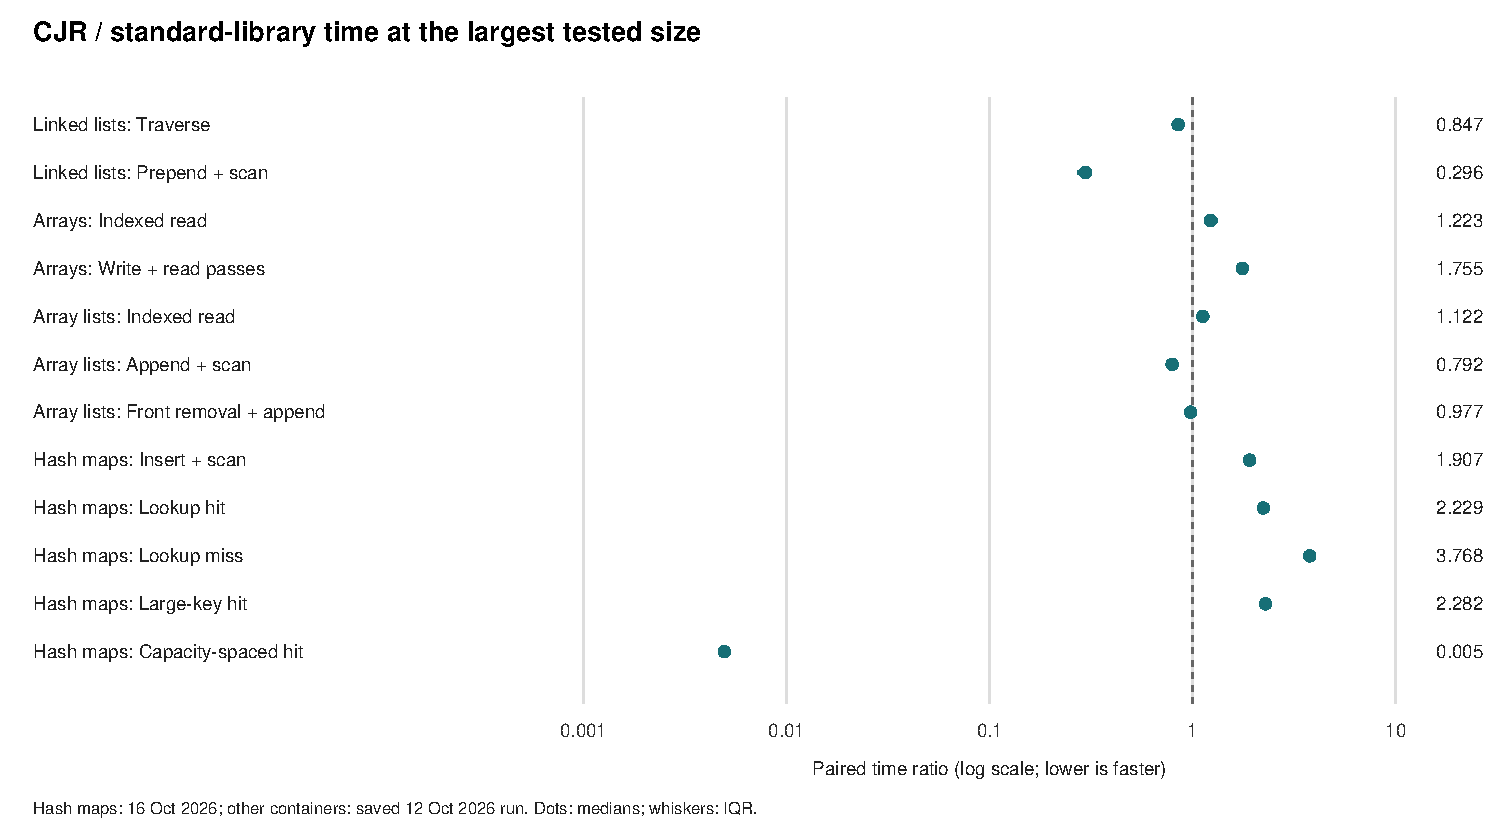
\includegraphics[width=\textwidth]{paper/figures/benchmark-overview.pdf}
\caption{Relative elapsed time of generated CJR and standard-library
workloads at their largest tested sizes.  The dashed line is equal time;
dots and error whiskers are the median and interquartile range of paired
CJR/standard ratios.  List build/scan, array-list build/scan, and map
build/scan include construction and growth; the other setups are excluded.}
\label{fig:benchmark-overview}
\end{figure}

\paragraph{Lists and arrays.} At the largest sizes, prepend-and-scan takes
0.296 times the standard-list time, and traversal 0.847 times.
Indexed array read takes 1.223 times the standard-array time, and
write/read 1.755 times. Representations, allocation, and runtime behavior
differ, so raw-pointer access alone does not imply a speed advantage.

\paragraph{Array lists.} Append-and-scan takes 0.792 times the standard
time, indexed read 1.122 times, and front rotation 0.977 times.
At $n=4096$, rotation takes 319.05 ns per remove/append pair versus
327.56 ns for the standard library. The proved suffix-copy loop is lowered
to overlap-safe \texttt{memmove}; this reduces the copying cost without
changing the linear number of words moved.

\paragraph{Hash maps.} At $n=16384$, successful lookup takes 5.36 ns
versus 2.43 ns for the standard library; misses take 6.33 versus 1.67 ns;
and insert-and-scan takes 35.04 versus 18.41 ns per inserted-and-read item.
Their median paired time ratios are 2.229, 3.768, and 1.907, respectively.
A median paired ratio need not equal the ratio of the two individual medians.
Large-key lookup takes 5.36 versus 2.36 ns at the same size.

The capacity-spaced workload has a different outcome: at $n=4096$, CJR
takes 5.03 ns per lookup versus 1021.15 ns for the standard map.
The separate CJR baseline immediately before the hash change took
3308.59 ns, so this case improved by about 658 times. Across its three
sizes, the before/after speedups range from 38 to 658 times.
This is a deliberately patterned workload, not a general lookup speedup.

Ordinary CJR hits and builds became 10--37\% slower than that baseline;
misses at 4096 and 16384 keys roughly doubled. The old hash placed
sequential keys into distinct consecutive buckets and the benchmark's
missing keys directly into the empty half of the table. Mixing adds
arithmetic and can require additional probes. At $n=16384$, CJR misses
rose from 3.13 to 6.33 ns. These are combined measurements; hashing,
probing, and memory-access costs have not been separately profiled.

\begin{figure}[!htbp]
\centering
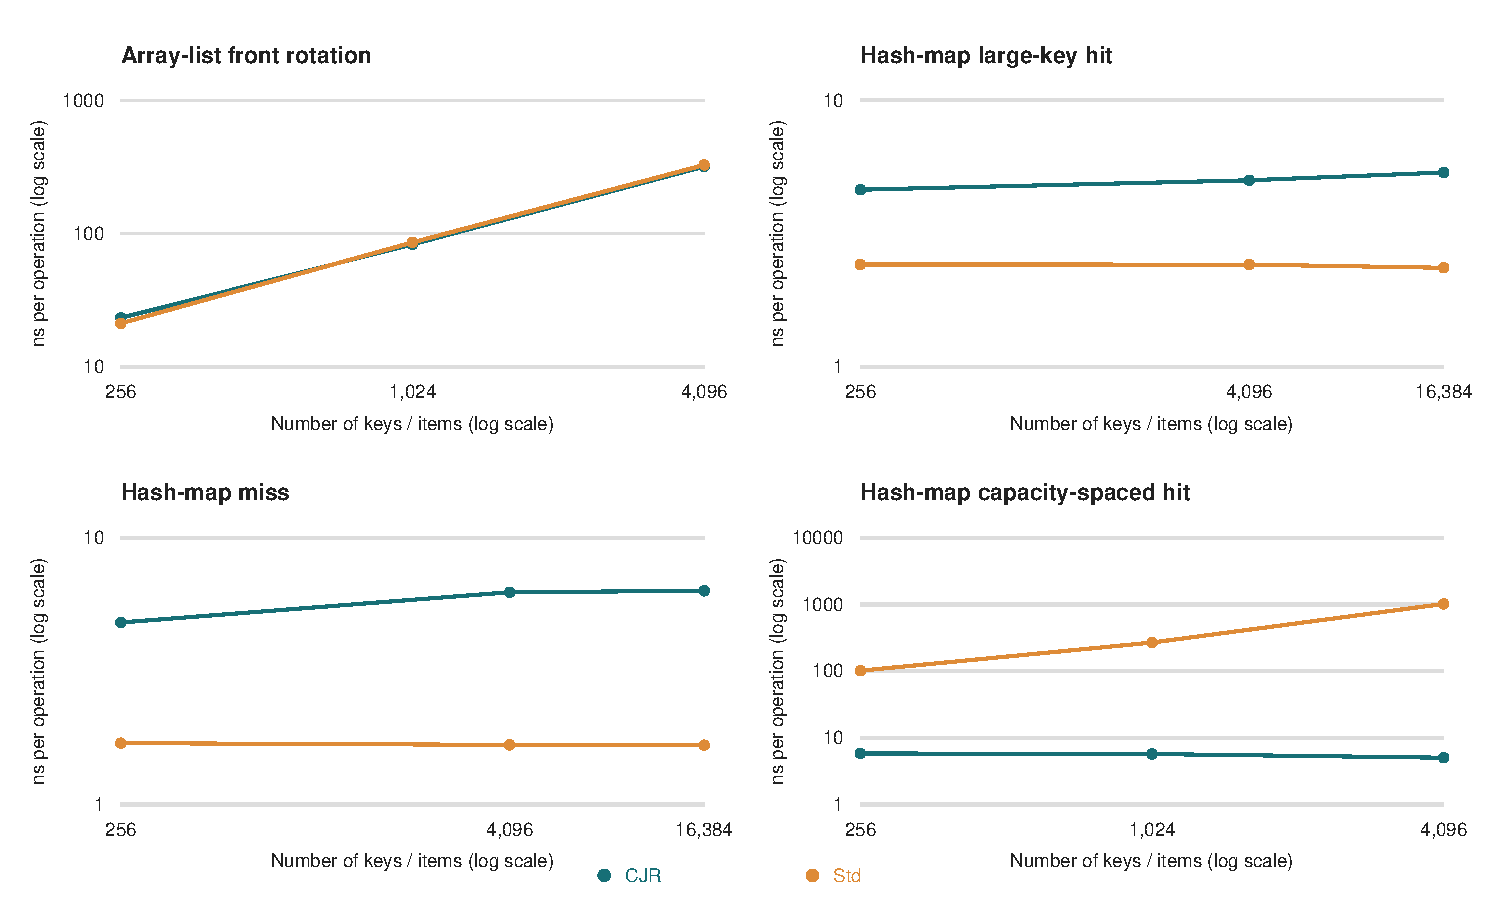
\includegraphics[width=\textwidth]{paper/figures/benchmark-scaling.pdf}
\caption{Scaling of front rotation and hash-map queries.  Both axes use
logarithmic scales.  Lines show individual median times, with interquartile
error whiskers. CJR capacity-spaced lookups remain near 5--6 ns across these sizes;
the standard-library curve grows with this key pattern.}
\label{fig:benchmark-scaling}
\end{figure}

\subsection{Interpretation, limitations, and reproduction}

The ArrayList representation remains contiguous. Front removal still moves
$n-1$ words, clears the old last word, and updates the live length and
version; append writes the freed end slot. Native bulk copying reduces the
cost of the shift without changing its linear complexity. The lowering
matches only the exact proved growth and removal bodies: their copies are
disjoint or overlap to the left. Arbitrary forward-copy loops remain
unchanged because right overlap can have different semantics from
\texttt{memmove}. The native FFI and printer remain outside the CJR proof.

CJR's \texttt{residue} performs one primitive signed remainder and at
most one addition, avoiding the old normalization loops. Primitive
allocation now emits zero-filled storage, matching the existing CJR
allocation rule on successful native allocations. The dedicated lookup
uses a bounded while loop, skips tombstones, and returns a two-field option
without insertion-hole tracking or recursive probe calls. Its functional
contract is proved against the same pure probe and map representation.

The new hash first reduces the key modulo 2147483647, multiplies by
1000000007, reduces by the same prime, and normalizes by capacity.
Compared with the former one-remainder hash, this uses three remainders
and one multiplication. The first reduction gives a proved \texttt{Int64}
bound for the product (\texttt{hash\_product\_int64}); it does not prove
machine-range safety for every operation or for arbitrary capacity growth.
The new distribution removes the systematic $i(2n)$ collision pattern in
these measurements. Keys separated by the hash prime still collide, and
linear probing remains; the hash is not adversarially secure.

The generated resizable buffers never free their old raw
blocks.  The harness does not repair that behavior or free buffers; batch
limits and process exits bound the experiment's allocation pressure.
Standard arrays and collections use the managed runtime instead.  This
comparison includes their natural allocation costs, but it is not a
measurement of sustained memory consumption or the cost of reclamation
that a production raw-memory implementation would need.

Primitive allocation now prints \texttt{calloc}, supplying zero-filled
storage on successful allocations as required by CJR's existing rules.
The array timings still exclude construction and explicitly write every
cell before reading it. The allocation repair and its remaining boundaries
are discussed in Appendix~\ref{sec:limitations}. The tests use valid indexes, bounded
values, a warm working set, and single-threaded code on an unpinned desktop
process.  They support workload-specific comparisons on this machine,
not a general correctness, complexity, or performance theorem.

The table and figures are regenerated from the latest saved per-example
measurements. The lists, arrays, and array-list rows retain the 12 October
run; only the hash-map rows use the 16 October run. Differences between
runs do not isolate every compiler or implementation effect: desktop
scheduling, calibration, and runtime variation can also affect timings.

The reproducible harnesses and configurations are in each example's
\texttt{benchmark/} directory. The shared runner in
\texttt{tools/project\_tools/benchmark.py} stores normalized raw samples,
source hashes, compiler settings, summaries, charts, and offline HTML.
Run \texttt{make benchmark} to collect new timings, or
\texttt{make project-report EXPLANATIONS=offline}
with \texttt{REPORT\_FLAGS=--allow-stale} to refresh HTML using
saved measurements. Run \texttt{python3 paper/update\_benchmarks.py}
with ReportLab installed to regenerate the manuscript table and figures,
then \texttt{make cj} to rebuild this PDF.

The generic HTML chart renderer was corrected on 16 October: its former
dot positions depended on map size and implementation but did not encode
the measured median. The corrected plots place medians and quartile
endpoints on a shared time axis. Raw timings and numeric summaries were
unaffected. The manuscript figures now also derive from the saved samples;
rebuilding documentation does not rerun the benchmark or change provenance.

\section{Most frequent integer: paired sort and scan}
\label{sec:most-frequent}

This example takes an initialized array of integers and returns its most
frequent value. An empty array returns \texttt{None}. If several values
have the same maximum frequency, the result is the value encountered first
in the original array. For example, $[8,3,3,8]$ returns $8$, even though
$3$ is numerically smaller. The input is preserved.

\paragraph{Verification status.}
Rocq checks the abstract specification, the complete functional
sort-and-scan correctness theorem, and an Iris weakest-precondition proof
of the actual CJR operation for both empty and nonempty inputs.
The proof includes allocation, input copying, paired Lomuto quicksort,
run scanning, the first-occurrence tie rule, both temporary-buffer frees,
and preservation of the input. Checked expression equalities connect the
loop lemmas to the terms supplied to the printer. The emitted Cangjie
program is compiled, tested, and benchmarked; native compilation and the
printer are outside the CJR semantic proof, as described below.

\subsection{Specification in elementary mathematics}

Let $A=(a_0,\ldots,a_{n-1})$ and define
\[
 f_A(x)=\bigl|\{i:0\leq i<n\ \land\ a_i=x\}\bigr|,
 \qquad
 t_A(x)=\min\{i:0\leq i<n\ \land\ a_i=x\}.
\]
For absent values set $t_A(x)=n$. The required answer $r$ satisfies
\[
\begin{aligned}
 r=\mathrm{None}&\quad\Longleftrightarrow\quad n=0,\\
 r=\mathrm{Some}(x)&\quad\Longrightarrow\quad
 f_A(x)>0\ \land\ (\forall y\in\mathbb Z,\ f_A(y)\leq f_A(x))\\
 &\hspace{36mm}\land\
 (\forall y\in\mathbb Z,\ f_A(y)=f_A(x)\Rightarrow t_A(x)\leq t_A(y)).
\end{aligned}
\]
Among maximum-frequency values the first-index condition determines a
unique value: different values cannot occupy the same original index.

\paragraph{English readout.}
Return no value exactly when the input is empty. Otherwise return a value
that occurs in the input, occurs at least as often as every other integer,
and whose first occurrence is no later than the first occurrence of any
other equally frequent value. Comparing only values, or returning the
first group in numeric sort order, would violate this contract.

\subsection{Gallina specification}

The executable specification uses \texttt{count\_occ} for frequency and a
recursive search for the first index; \texttt{mf\_first\_index\_or\_len}
returns the array length for an absent value. Indices and counts are
natural numbers. Values are unbounded Rocq integers.
\begin{lstlisting}
Definition most_frequent_spec (xs : list Z) (answer : option Z) : Prop :=
  match xs, answer with
  | [], None => True
  | [], Some _ => False
  | _ :: _, None => False
  | _ :: _, Some x =>
      (mf_frequency x xs > 0)%nat /\
      (forall y, mf_frequency y xs <= mf_frequency x xs)%nat /\
      (forall y, mf_frequency y xs = mf_frequency x xs ->
         mf_first_index_or_len x xs <= mf_first_index_or_len y xs)%nat
  end.
\end{lstlisting}
The independently proved \texttt{mf\_choose xs xs} computes this answer by
counting each candidate against the whole input. It is a quadratic
reference oracle, not the efficient implementation. Its theorem
\texttt{mf\_choose\_correct} proves the specification by induction over
candidate order, retaining the earlier candidate on a frequency tie.

The verified functional implementation composes paired Lomuto sort,
adjacent-value grouping, and summary selection. Written with
\texttt{option\_map} in place of the equivalent source infix notation:
\begin{lstlisting}
Definition mf_sort_scan xs : option Z :=
  option_map fst (mf_best_summary (mf_run_summaries (mf_sorted_pairs xs))).

Theorem mf_sort_scan_correct xs :
  most_frequent_spec xs (mf_sort_scan xs).
\end{lstlisting}
This theorem has no summary-validity hypothesis: the grouping and sorting
proofs discharge it. It also includes the empty case and the specified
tie rule. The CJR refinement theorem below connects the concrete operation to this functional result.

\subsection{Algorithm walkthrough and pseudocode}

Copy the input into records $(a_i,i)$, represented by two parallel arrays.
Sorting these records lexicographically places equal values together and
orders their original indices within each group. Every swap moves both
fields. For $[8,3,3,8]$, the sorted records are
$[(3,1),(3,2),(8,0),(8,3)]$. Their summaries are $(3,2,1)$ and $(8,2,0)$,
where each triple is (value, count, first index). Both counts are two; the
second summary wins because index zero precedes index one.

\begin{lstlisting}
mostFrequent(A):
  n := length(A)
  if n = 0: return None
  values := copy(A); indices := [0, ..., n-1]
  quicksortPairs(values, indices, 0, n)  // half-open interval
  bestCount := 0; bestFirst := n; start := 0
  while start < n:
    x := values[start]; end := start + 1
    first := indices[start]
    while end < n:
      if values[end] != x: break
      first := min(first, indices[end]); end := end + 1
    count := end - start
    if count > bestCount or
       (count = bestCount and first < bestFirst):
      bestValue := x; bestCount := count; bestFirst := first
    start := end
  free(values.data); free(indices.data)
  return Some(bestValue)
\end{lstlisting}
Lomuto partition uses the last record as pivot. It maintains a boundary
$i$ and visits records $j$ from \texttt{lo} through \texttt{hi-2}; records
at most the pivot are swapped into the left prefix. The pivot is then
swapped into position $i$. Recursion sorts $[\texttt{lo},i)$ and
$[i+1,\texttt{hi})$, leaving the pivot out of both recursive calls.

Under the usual random-order assumption for the distinct paired keys,
quicksort takes expected $O(n\log n)$ comparisons; its worst case is
$O(n^2)$. This implementation does not randomize pivots. Sorted,
reverse-sorted, and all-equal \emph{value} inputs can be particularly poor:
in the all-equal case the increasing original indices already put the
paired keys in sorted order. Copying and scanning take $O(n)$. The two
buffers require $O(n)$ space; recursive stack depth is $O(n)$ in the worst
case. Both raw buffers are freed before returning.

\subsection{Formal CJR implementation and emitted Cangjie}

The implementation lives in \texttt{example/most\_frequent/rocq/most\_frequent.v}
as core-language expressions \texttt{mf\_swap\_body},
\texttt{mf\_partition\_body}, \texttt{mf\_qsort\_body}, and
\texttt{mf\_body}. A pair comparison is expressed using the available
\texttt{LeOp} and \texttt{If}; it never subtracts two input values or adds
one to an input value, so comparisons also work at the \texttt{Int64}
boundaries. The group condition uses an explicit \texttt{If} because CJR's
\texttt{AndOp} evaluates both operands. An eager conjunction containing a
raw read at \texttt{end == n} would access beyond the array.

\begin{lstlisting}
If (BinOp LeOp (Var "v") (Var "pv"))
  (If (BinOp LeOp (Var "pv") (Var "v"))
    (BinOp LeOp (Var "ix") (Var "pi"))
    (Val (LitV (LitBool true))))
  (Val (LitV (LitBool false)))
\end{lstlisting}
The following is the complete core-language definition of the pair swap,
partition, recursive sort, copy, and group scan. Calls package their
arguments in a structural value, \texttt{VarBind} introduces mutable stack
variables, and \texttt{Assign} updates those variables. The loop guards,
array reads, and final block frees are therefore explicit syntax subject
to the CJR semantics.
\lstinputlisting[firstline=179,lastline=269,basicstyle=\ttfamily\footnotesize]{example/most_frequent/rocq/most_frequent.v}

The printer uses these expressions directly through
\texttt{p\_most\_frequent}; \texttt{make cj} regenerates the following
standalone program. \texttt{Int64Option(false,0)} represents
\texttt{None}; its numeric field has no meaning in that case.
\lstinputlisting{example/most_frequent/extracted/most_frequent.cj}

The input must have a correct length and valid initialized storage at
every in-range index. The empty case reads only the length field and
allocates no temporary buffers. The tests construct an empty view over a
positive allocation instead of depending on \texttt{malloc(0)}. The full
native storage contract also requires allocation byte sizes and indices
to fit their machine types. As elsewhere in this tutorial, a Rocq proof
over unbounded integers does not by itself establish the compiler's
\texttt{Int64} arithmetic and allocation behavior.

\subsection{Correctness argument and checked components}

\paragraph{Record preservation.}
\texttt{mf\_pair\_swap\_perm} proves that swapping two records preserves
the record multiset, including self-swaps and out-of-range no-op cases in
the functional model. Induction on partition fuel lifts this to
\texttt{mf\_lomuto\_perm}. The final pivot swap preserves the same
multiset, proving \texttt{mf\_partition\_perm}. Induction on recursive
fuel composes the two recursive permutations and the partition
permutation, proving \texttt{mf\_qsort\_perm}. It follows that no original
(value,index) record is lost or duplicated by the functional sort.

\paragraph{Ordering.}
For a positive width $w$ larger than every record index, define the
\emph{proof-only} rank $\rho_w(x,i)=xw+i$. If $x<y$, then
$\rho_w(x,i)<\rho_w(y,j)$ because $0\leq i,j<w$; if $x=y$, comparing ranks
is exactly comparing indices. Conversely, a rank comparison cannot put a
larger value before a smaller value, since an index difference has
magnitude less than $w$. Lemma \texttt{mf\_rank\_order} checks this
argument with integer arithmetic. Lemmas \texttt{mf\_swap\_map},
\texttt{mf\_lomuto\_map}, \texttt{mf\_partition\_map}, and
\texttt{mf\_qsort\_slice\_map} show that mapping records to ranks commutes
with the actual functional Lomuto operations. The existing scalar
quicksort ordering theorem therefore yields \texttt{mf\_qsort\_sorted}.
For input records, \texttt{mf\_pairs\_bounded} supplies $w=n$ when $n>0$.
No rank is computed in the emitted program.

\paragraph{Frequency and provenance.}
\texttt{mf\_pairs\_values} proves that projecting original records gives
exactly the input. Mapping the sort permutation through that projection
preserves every frequency, which is
\texttt{mf\_sorted\_pairs\_frequency}. The lookup lemma and permutation
also prove \texttt{mf\_sorted\_pairs\_origin}: every sorted record's
index points to its value in the original input. This is stronger than
preserving a multiset of values alone.

\paragraph{Grouping obligation.}
In a lexicographically sorted record sequence, all records with value $x$
form one contiguous run. A different value between two $x$ records would
have to be both at least $x$ and at most $x$, contradicting its difference.
Scanning from the run's first record until the first different value
therefore visits exactly all $x$ records. Its length is $f_A(x)$ and the
minimum original index is $t_A(x)$. To mechanize the imperative scan, the
inner invariant must state that $[\texttt{start},\texttt{end})$ is exactly
the portion of this run already visited, and that \texttt{first} is the
minimum index there. It must also retain ownership of both buffers and
establish each read is in bounds. The functional grouping is now checked: \texttt{mf\_run\_summaries\_sound} proves that each summary has its global
frequency, a witnessed minimum original index, and positive count, that
summary keys do not repeat, and that all record values are represented.
The functional scan builds the same adjacent-value groups by structural
recursion from the tail, extending the first summary when its value agrees
with the current record. Its induction uses sortedness to exclude an
earlier value from every later, different-value group. The forward-loop invariant and its refinement of this grouping are proved
by the concrete scan lemmas described below.

\paragraph{Selection.}
A summary $s$ has value, count, and first-index fields. Its score is better
than another summary when its count is larger, or its count is equal and
its first index is no larger. The checked lemmas establish a total,
transitive score order. \texttt{mf\_best\_summary\_sound} proves by
induction that the selected summary belongs to the list and dominates
every other summary. The theorem \texttt{mf\_summary\_selection\_correct}
then establishes \texttt{most\_frequent\_spec}, provided all summaries
have their true positive frequencies and first indices, and every input
value has a summary. Absent values have frequency zero, so the domination
condition extends to all integers. The checked theorem \texttt{mf\_run\_summaries\_complete} now establishes
that precondition for the actual functional groups of the paired sort.
Permutation transfers the minimum-index witnesses back to the original
input; \texttt{mf\_first\_index\_attained} and
\texttt{mf\_first\_index\_minimum} show that this minimum is exactly the
specification's first-occurrence index. Composing these results gives
\texttt{mf\_sort\_scan\_correct}, a correctness theorem for the complete
functional algorithm rather than only the independent quadratic oracle.

\paragraph{Concrete paired-array Iris proof.}
The predicate \texttt{mf\_pair\_arrays ps oa ob} owns two initialized arrays:
one contains the value projection of the record list, and the other
contains the original-index projection, embedded from naturals into
integers. \texttt{mf\_swap\_arrays\_wp} checks all four reads and all four
writes of the actual swap body. On a self-swap the two initial lookup
facts imply the read values agree, which justifies the second write after
the first update. Mapping the functional record swap through both
projections gives \texttt{mf\_swap\_pairs\_wp}.

\texttt{mf\_lex\_compare\_wp} proves the concrete nested comparisons return
exactly \texttt{mf\_pair\_leb}. Each partition iteration reads the current
record, applies this comparison, optionally swaps it into the stored
prefix and increments $i$, then increments $j$.
\texttt{mf\_partition\_step\_wp} accounts for both arrays and both mutable
stack cells throughout that step. Induction on the remaining scan length,
$(\texttt{hi}-1)-j$, yields \texttt{mf\_partition\_scan\_wp}: its result is
exactly the functional \texttt{mf\_lomuto} result and its final $j$ is
\texttt{hi-1}. The induction maintains $i\leq j\leq\texttt{hi-1}$ and
\texttt{hi-1} below the array length, so both record reads and swaps are
in bounds. Equality lemmas extract the loop directly from
\texttt{mf\_partition\_body} and check that it is the expression proved by
these step and scan theorems.

\texttt{mf\_partition\_wp} opens the two local stack variables, reads the
last record as pivot, applies the scan theorem, performs the final pivot
swap, and returns the functional partition index. It returns both array
representations and supplies the stack cells for their lexical scope
cleanup. The bound $\texttt{lo}\leq p<\texttt{hi}$ makes both recursive
subintervals strictly shorter. Induction on a fuel at least
$\texttt{hi}-\texttt{lo}$ then proves \texttt{mf\_qsort\_slice\_wp} for the
actual recursive CJR function. Its postcondition is the exact functional
\texttt{mf\_qsort\_slice} array contents, not merely an assertion that some
sorted list exists. At full length, \texttt{mf\_qsort\_wp} therefore connects
the emitted paired quicksort to the previously proved sorted-permutation
model. No abstract comparator or swap correctness is assumed here.

\paragraph{Complete-buffer cleanup.}
The new \texttt{mf\_wp\_free\_block} rule owns a block token for the exact
buffer length and all of its raw cells. Its proof deletes the cells in
reverse index order from the Iris ghost map, deletes the block token,
and uses \texttt{mf\_wf\_free\_block} to preserve the state invariant.
Disjoint live blocks retain their cells: the deleted interval cannot
intersect any of their intervals. \texttt{mf\_release\_array\_wp} applies
this rule to the actual \texttt{Free(FieldLoad(array,1))} expression.
\texttt{mf\_cleanup\_wp} composes the two final frees and result
construction while framing ownership of the unchanged input array.
The cleanup preserves the already selected scalar value; it reads no
buffer cell after freeing a buffer.

\paragraph{Copying and initialization.}
For input $A$ of length $n$, after $j$ copy iterations in the CJR
allocation model the value buffer is
\[
 \mathrm{take}(j,A)\mathbin{+\!+}\mathrm{replicate}(n-j,0),
\]
and the index buffer is $[0,\ldots,j-1]$ followed by $n-j$ zero cells.
The zero suffix describes the modeled allocation. The emitted native
routine writes every temporary cell before reading it, so this operation
explicitly initializes the copied records even though the printer now
uses zero-filled \texttt{calloc} storage.
The initialized prefix grows by one cell on each iteration. The loop
condition supplies $j<n$, justifying the source read and both destination
writes. Ownership of the input is retained throughout. At $j=n$, the
buffers are exactly the two projections of \texttt{mf\_pairs A 0}.
\texttt{mf\_copy\_step\_wp} proves the actual nested read/write step;
\texttt{mf\_copy\_loop\_wp} proves the loop by induction on $n-j$.
\texttt{mf\_copy\_loop\_is\_code} is an expression equality obtained from
\texttt{mf\_body}, so a separate copy program cannot satisfy this proof
in place of the emitted one.

\paragraph{Concrete run and winner scan.}
The pure helper \texttt{mf\_scan\_run value first suffix} returns the
number of additional equal-value records and the minimum original index
including the already visited records. It stops on an empty suffix or a
different value. \texttt{mf\_group\_inner\_wp} proves the actual guarded
inner loop computes exactly this pair: if the loop starts at position
$j$ with minimum $t$, it finishes at $j+\mathrm{extra}$ with the computed
minimum. Its induction follows the unread suffix. An exhausted suffix
implies $j=n$; the explicit conditional returns false without loading a
cell. A nonempty suffix implies $j<n$, so the equality test is safe.
On a matching record, the index read is safe, the conditional minimum
update preserves its stack cell, and advancing the cursor decreases the
unread suffix. A different value leaves the cursor and minimum unchanged.
The theorem retains both arrays and both mutable stack cells in every case.

\texttt{mf\_group\_summary\_decomposition} connects this forward scan
to \texttt{mf\_run\_summaries}: for a first record $p$ and suffix $P$,
scanning the additional equal records produces the first summary
$(p.\mathrm{value},1+\mathrm{extra},\mathrm{minimum})$, and the remaining
summaries are exactly those of the suffix after dropping those records.
The proof combines adjacent summaries; count addition and minimum are
associative. Thus the forward implementation and the tail-recursive
functional grouping agree, without assuming that agreement as a precondition.

\texttt{mf\_strict\_better} uses a larger count, or an equal count and a
strictly smaller first index, exactly as the native operation does.
\texttt{mf\_fold\_best\_sound} proves that the accumulated winner is one
of the seed and processed summaries and dominates all of them in the
score order. The seed has count zero. Every real summary has positive
count, so a nonempty completed scan cannot select the seed.
\texttt{mf\_forward\_scan\_correct} combines this fact, completeness of
all run summaries, and the score order to prove the specification.

The concrete update lemmas prove the nested count/tie comparison and all
three assignments to the best-value, best-count, and best-first stack cells.
\texttt{mf\_group\_step\_wp} composes the first-record reads, creation of
local end/minimum cells, inner loop, summary selection, and cursor update.
It also returns the local stack ownership required for scope cleanup.
\texttt{mf\_group\_outer\_wp} proves the full outer loop by induction
on a fuel at least the unread suffix length. Each iteration consumes at
least its first record; its next cursor is in bounds and its remaining
suffix is shorter. Its final best cells contain the exact
\texttt{mf\_forward\_scan} result. Checked expression equalities link
both loops to \texttt{mf\_body}.

\paragraph{Complete Iris contract.}
The input predicate handles the empty header separately because the
CJR raw-allocation model requires positive block lengths:
\begin{lstlisting}
Definition mf_input `{!cjrGS Σ} (xs : list Z) oi : iProp Σ :=
  match xs with
  | [] => ObjId oi ↦ₒ[0] LitV (LitInt 0)
  | _ :: _ => is_array xs (LitV (LitObj oi))
  end.
\end{lstlisting}
Here $\mapsto_o[0]$ denotes ownership of object field zero. The empty case requires only the zero length field because the
operation reads no element or pointer and allocates nothing.
The positive case owns the initialized input array, including its exact
length, data pointer, raw-block token, and element cells.
\texttt{mf\_option\_value} encodes \texttt{None} as the false/zero result
structure and \texttt{Some x} as the true/$x$ structure.
The checked complete theorem is
\[
 \mathrm{mfInput}(A,a)\ \vdash\
 \mathrm{WP}\ \mathrm{mostFrequent}(a)\
 \{v.\ \lceil v=\mathrm{encode}(\mathrm{mfSortScan}(A))\rceil
       *\mathrm{mfInput}(A,a)\}.
\]
\par\noindent
\begin{minipage}{\textwidth}
\begin{lstlisting}
Theorem mf_wp `{!cjrGS Σ} `{!invGS_gen HasLc Σ} xs oi :
  mf_input xs oi -∗
  WP App (Rec None (Some "input") mf_body) (Val (LitV (LitObj oi)))
    {{ v, ⌜v = mf_option_value (mf_sort_scan xs)⌝ ∗ mf_input xs oi }}.
\end{lstlisting}
\end{minipage}\par
The connective $-\!* $ is separating implication: it consumes the
input ownership to establish the weakest-precondition assertion. The
postcondition combines a pure result equality with ownership of the same
input using separating conjunction.
\texttt{mf\_nonempty\_wp} proves allocation of two positive-length
buffers, applies the copy and quicksort theorems, initializes the winner
and cursor cells, then applies the outer scan theorem. The actual final
\texttt{Free} expressions consume both temporary raw buffers. The result
is read from the best-value stack cell after cleanup. The input ownership
is framed throughout and returned unchanged. The proof supplies all local
stack cells for lexical scope cleanup.
\texttt{most\_frequent\_spec\_unique} shows that two answers satisfying
the specification are equal: their maximum frequencies agree, their first
indices agree, and the input cell at that index determines their value.
It identifies the forward scan's answer with \texttt{mf\_sort\_scan}.
\texttt{mf\_wp} combines this nonempty proof with \texttt{mf\_empty\_wp};
\texttt{mf\_spec\_wp} adds the specification to its postcondition.
No copying, grouping, comparator, or sorting hypothesis is assumed for
this contract. The representative project assumption audit checks
88 theorems, including the complete operation and its kernels.

\subsection{Testing and comparative benchmarks}

Eleven Cangjie unit-test methods pass against the emitted source: empty,
singleton, all-equal, all-distinct, interleaved two-way and three-way ties,
negative and boundary integers, sorted and reversed inputs, exhaustive
small arrays, and paired-sort preservation. The exhaustive test checks all
3,280 arrays of lengths zero through seven over $\{-1,0,1\}$ against an
independent quadratic reference. Every result test also checks that the
input is unchanged. The pair test checks lexicographic order, distinct
original indices, and each value's correspondence to its original index.
Tests check native behavior in addition to the CJR refinement proof;
they do not prove the printer or native compiler correct.

The baselines are explicitly written equivalent operations using the
SDK's \texttt{std.sort.sort} and \texttt{std.collection.HashMap}. They
are not built-in most-frequent functions. The sort baseline sorts an array
of original indices with a value/index comparator and scans equal-value
runs. The HashMap baseline counts and maintains the maximum count in one
pass, then visits the original input until it finds a value with that
count, preserving first-occurrence semantics. All return the same option
encoding, preserve the input, and check the empty case.

The measurements were rerun on 9 October 2026. The compiler is Cangjie 1.0.5 cjnative at \texttt{-O2}, targeting
\texttt{aarch64-apple-darwin}, on an Apple M4 Mac mini with 16 GB RAM and
macOS 26.6.2. Three independent sequential processes each record seven
samples per implementation at each workload/size point: 693 measurements
in total. Each operation receives identical preconstructed values. Timing
includes its allocations, copying or map construction, sorting/counting,
scan, result construction, and the CJR buffer frees. Input setup, warmups,
checksums, and printing are outside the timer. Each implementation receives
two warmup calls. Batch repetitions are $262144/n$ for all implementations;
trial order rotates through the three implementations. There is no core
pinning, forced garbage collection, or subtraction of loop overhead.

The deterministic distributions are
$a_i=((37i)\bmod101)-50$ (dense),
$a_i=((48271i)\bmod n)-n/2$ (distinct permuted values), and
$a_i=((17i)\bmod7)-3$ (seven values), at $n=256,4096,16384$.
Sorted and reverse-sorted distinct inputs are measured only at $n=256$
to bound the cost of the deliberately reused quadratic worst case.
These workloads are not random samples from all input distributions.
Raw results, source hashes, compiler metadata, and reproducible runners
are in \texttt{example/most\_frequent/benchmark/results/} and
\texttt{tools/project\_tools/benchmark.py}.

\begin{figure}[H]
\centering
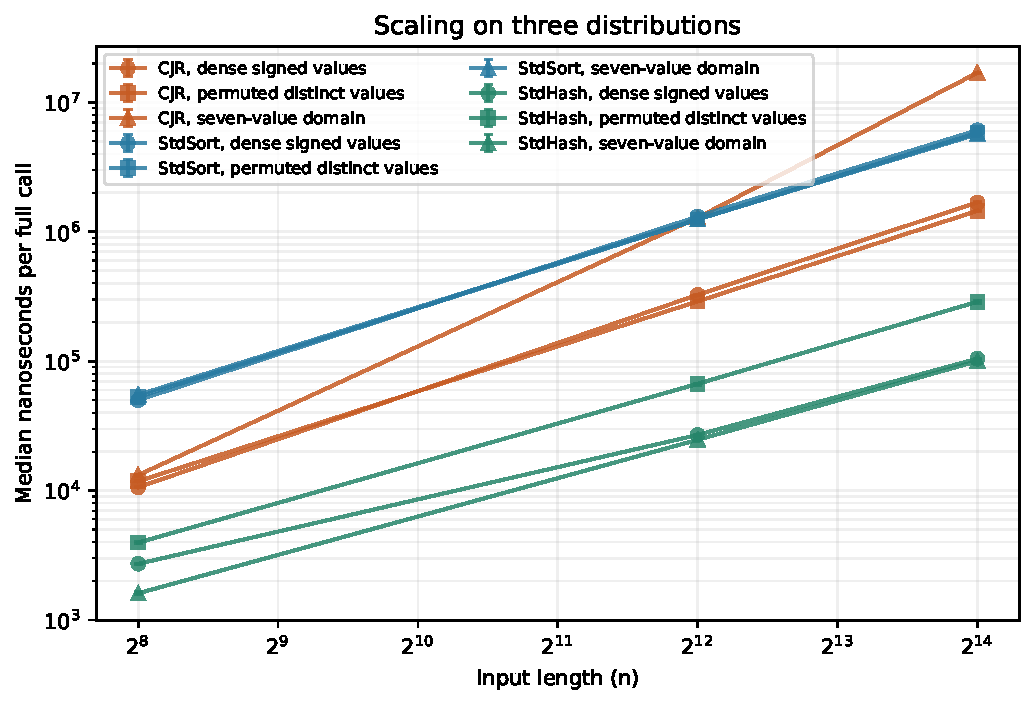
\includegraphics[width=\textwidth]{example/most_frequent/docs/figures/most-frequent-scaling.pdf}
\caption{Complete-operation timings: median elapsed time per call;
error bars show the interquartile range across 21 samples.}
\label{fig:most-frequent-benchmark}
\end{figure}
\begin{figure}[H]
\centering
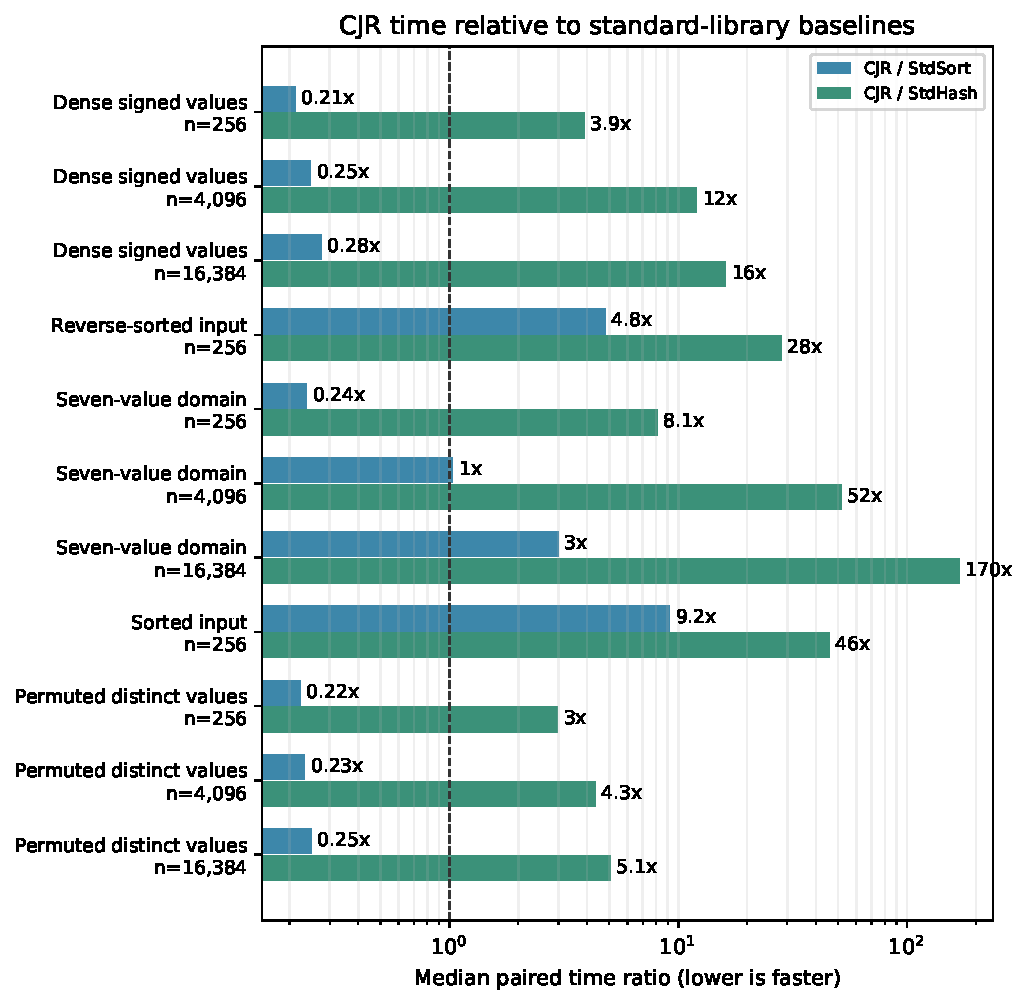
\includegraphics[width=\textwidth]{example/most_frequent/docs/figures/most-frequent-ratios.pdf}
\caption{Median paired CJR/baseline ratios. Values above one mean CJR is slower.}
\end{figure}
\begin{table}[H]
\centering\small
\begin{tabular}{lrrrr}
\hline
Distribution & $n$ & CJR ($\mu$s) & std.sort ($\mu$s) & HashMap ($\mu$s) \\
\hline
Dense signed values & 256 & 10.59 & 49.97 & 2.72 \\
Dense signed values & 4,096 & 325.64 & 1,311.50 & 26.92 \\
Dense signed values & 16,384 & 1,686.50 & 6,093.56 & 104.44 \\
Reverse-sorted input & 256 & 111.48 & 23.08 & 3.91 \\
Seven-value domain & 256 & 13.18 & 54.86 & 1.61 \\
Seven-value domain & 4,096 & 1,284.67 & 1,245.78 & 24.69 \\
Seven-value domain & 16,384 & 16,920.25 & 5,675.75 & 100.06 \\
Sorted input & 256 & 179.50 & 19.51 & 3.91 \\
Permuted distinct values & 256 & 11.81 & 52.92 & 3.96 \\
Permuted distinct values & 4,096 & 289.81 & 1,243.81 & 66.83 \\
Permuted distinct values & 16,384 & 1,451.50 & 5,797.94 & 287.88 \\
\hline
\end{tabular}
\caption{Median time per complete operation; 21 samples per entry.}
\end{table}


These measurements compare complete implementations with different
representations and runtime costs. CJR uses unchecked raw accesses; the
sort baseline uses standard arrays and a comparator that reads the input
through their API. CJR allocates two buffers whereas that baseline
allocates one index array. Consequently a speed difference does not
isolate the sorting algorithm. The seven-value and already ordered cases
expose the pivot strategy's weakness. The HashMap alternative avoids
sorting and can be substantially faster, but relies on hashing behavior
and a different verification effort. No timing establishes correctness,
a general performance ranking, or worst-case bounds for the SDK's map.


\section{Limitations and target-code risks}
\label{sec:limitations}
CJR integers are unbounded mathematical integers, while generated Int64 values
have machine bounds. Callers must satisfy the stated arithmetic and memory
bounds. The logic specifies a sequential fragment and does not prove a full
Cangjie type-soundness theorem, native compiler correctness, or the behavior
of operating-system and frontend code. Generic specifications quantify over
resource representations; they are not a universal relational-parametricity
result. Checked kernels and conditional refinement contracts must be read
with their hypotheses and documented coverage. Proofs were not rerun during
this migration, and runtime tests supply separate empirical evidence.

\section{Migration and current runtime evidence}
Proofs were not revalidated during this repository split. Historical proof reports retain their original dates and provenance. Runtime timings measure generated native programs and do not establish cryptographic security or compiler correctness.
\subsection{Measurement protocol}
Timings are from optimized Cangjie 1.0.5 builds on the machine recorded in each metadata file. Each suite uses its checked-in configuration, warmups, independent processes, and checksum validation. Medians and interquartile ranges describe repeated samples; they are not universal guarantees.\par
\subsection{example/array/benchmark/results}
Recorded 2026-10-29T14:14:58.538369+00:00. 12 workload groups. Values below are ns per harness-defined operation. Full results, provenance, and charts are in the local HTML report.
\begin{longtable}{p{0.57\textwidth}rr}Workload / implementation & Median & IQR \\ \hline
array\_read / 256 / CJR & 0.96 & 0.01 \\
array\_read / 256 / Std & 0.64 & 0.01 \\
array\_read / 4096 / CJR & 0.95 & 0.01 \\
array\_read / 4096 / Std & 0.63 & 0.01 \\
array\_read / 65536 / CJR & 0.98 & 0.01 \\
array\_read / 65536 / Std & 0.72 & 0.08 \\
array\_write\_read / 256 / CJR & 0.86 & 0.10 \\
array\_write\_read / 256 / Std & 0.53 & 0.01 \\
array\_write\_read / 4096 / CJR & 0.84 & 0.10 \\
array\_write\_read / 4096 / Std & 0.51 & 0.01 \\
array\_write\_read / 65536 / CJR & 0.90 & 0.10 \\
array\_write\_read / 65536 / Std & 0.56 & 0.01 \\
\end{longtable}
\subsection{example/array\_list/benchmark/results}
Recorded 2026-10-29T14:15:08.807320+00:00. 18 workload groups. Values below are ns per harness-defined operation. Full results, provenance, and charts are in the local HTML report.
\begin{longtable}{p{0.57\textwidth}rr}Workload / implementation & Median & IQR \\ \hline
arraylist\_build\_scan / 16384 / CJR & 3.78 & 0.26 \\
arraylist\_build\_scan / 16384 / Std & 4.10 & 0.36 \\
arraylist\_build\_scan / 256 / CJR & 4.41 & 0.25 \\
arraylist\_build\_scan / 256 / Std & 4.23 & 0.78 \\
arraylist\_build\_scan / 4096 / CJR & 3.77 & 0.20 \\
arraylist\_build\_scan / 4096 / Std & 4.18 & 0.38 \\
arraylist\_read / 16384 / CJR & 0.95 & 0.01 \\
arraylist\_read / 16384 / Std & 0.84 & 0.01 \\
arraylist\_read / 256 / CJR & 0.97 & 0.01 \\
arraylist\_read / 256 / Std & 0.85 & 0.00 \\
arraylist\_read / 4096 / CJR & 0.95 & 0.03 \\
arraylist\_read / 4096 / Std & 0.83 & 0.02 \\
arraylist\_rotate / 1024 / CJR & 81.62 & 6.13 \\
arraylist\_rotate / 1024 / Std & 76.62 & 2.20 \\
arraylist\_rotate / 256 / CJR & 22.20 & 0.11 \\
arraylist\_rotate / 256 / Std & 19.99 & 0.31 \\
arraylist\_rotate / 4096 / CJR & 309.75 & 9.13 \\
arraylist\_rotate / 4096 / Std & 319.15 & 5.51 \\
\end{longtable}
\subsection{example/hash\_map/benchmark/results}
Recorded 2026-10-29T14:15:54.612223+00:00. 30 workload groups. Values below are ns per harness-defined operation. Full results, provenance, and charts are in the local HTML report.
\begin{longtable}{p{0.57\textwidth}rr}Workload / implementation & Median & IQR \\ \hline
hashmap\_build\_scan / 16384 / CJR & 35.73 & 0.90 \\
hashmap\_build\_scan / 16384 / Std & 19.02 & 2.07 \\
hashmap\_build\_scan / 256 / CJR & 32.37 & 0.79 \\
hashmap\_build\_scan / 256 / Std & 16.85 & 0.46 \\
hashmap\_build\_scan / 4096 / CJR & 37.73 & 0.53 \\
hashmap\_build\_scan / 4096 / Std & 17.25 & 0.80 \\
hashmap\_collision / 1024 / CJR & 5.60 & 0.24 \\
hashmap\_collision / 1024 / Std & 262.78 & 4.83 \\
hashmap\_collision / 256 / CJR & 5.45 & 0.47 \\
hashmap\_collision / 256 / Std & 98.51 & 2.40 \\
hashmap\_collision / 4096 / CJR & 4.93 & 0.09 \\
hashmap\_collision / 4096 / Std & 997.68 & 19.96 \\
hashmap\_hit / 16384 / CJR & 5.22 & 0.07 \\
hashmap\_hit / 16384 / Std & 2.30 & 0.04 \\
hashmap\_hit / 256 / CJR & 4.72 & 0.19 \\
hashmap\_hit / 256 / Std & 2.46 & 0.03 \\
hashmap\_hit / 4096 / CJR & 4.84 & 0.10 \\
hashmap\_hit / 4096 / Std & 2.30 & 0.05 \\
hashmap\_miss / 16384 / CJR & 6.04 & 0.34 \\
hashmap\_miss / 16384 / Std & 1.63 & 0.02 \\
hashmap\_miss / 256 / CJR & 4.86 & 0.27 \\
hashmap\_miss / 256 / Std & 1.66 & 0.03 \\
hashmap\_miss / 4096 / CJR & 5.79 & 0.83 \\
hashmap\_miss / 4096 / Std & 1.65 & 0.03 \\
hashmap\_wide\_key / 16384 / CJR & 5.29 & 0.10 \\
hashmap\_wide\_key / 16384 / Std & 2.31 & 0.03 \\
hashmap\_wide\_key / 256 / CJR & 4.62 & 0.20 \\
hashmap\_wide\_key / 256 / Std & 2.46 & 0.05 \\
hashmap\_wide\_key / 4096 / CJR & 4.96 & 0.12 \\
hashmap\_wide\_key / 4096 / Std & 2.33 & 0.02 \\
\end{longtable}
\subsection{example/list/benchmark/results}
Recorded 2026-10-29T14:15:26.333393+00:00. 12 workload groups. Values below are ns per harness-defined operation. Full results, provenance, and charts are in the local HTML report.
\begin{longtable}{p{0.57\textwidth}rr}Workload / implementation & Median & IQR \\ \hline
list\_build\_scan / 16384 / CJR & 4.22 & 0.09 \\
list\_build\_scan / 16384 / Std & 14.71 & 0.69 \\
list\_build\_scan / 256 / CJR & 4.12 & 0.09 \\
list\_build\_scan / 256 / Std & 14.74 & 0.58 \\
list\_build\_scan / 4096 / CJR & 4.10 & 0.66 \\
list\_build\_scan / 4096 / Std & 14.77 & 0.99 \\
list\_traverse / 16384 / CJR & 1.80 & 0.07 \\
list\_traverse / 16384 / Std & 2.12 & 0.14 \\
list\_traverse / 256 / CJR & 1.73 & 0.02 \\
list\_traverse / 256 / Std & 2.17 & 0.02 \\
list\_traverse / 4096 / CJR & 1.78 & 0.27 \\
list\_traverse / 4096 / Std & 2.26 & 0.08 \\
\end{longtable}
\subsection{example/list\_rev/benchmark/results}
Recorded 2026-10-29T14:15:33.045379+00:00. 6 workload groups. Values below are ns per harness-defined operation. Full results, provenance, and charts are in the local HTML report.
\begin{longtable}{p{0.57\textwidth}rr}Workload / implementation & Median & IQR \\ \hline
list\_reverse / 16384 / CJR & 34258.79 & 2808.59 \\
list\_reverse / 16384 / Native & 22028.32 & 1546.88 \\
list\_reverse / 256 / CJR & 440.67 & 1.19 \\
list\_reverse / 256 / Native & 194.45 & 9.34 \\
list\_reverse / 4096 / CJR & 7955.32 & 471.92 \\
list\_reverse / 4096 / Native & 4667.85 & 654.05 \\
\end{longtable}
\subsection{example/most\_frequent/benchmark/results}
Recorded 2026-10-29T14:16:30.163972+00:00. 33 workload groups. Values below are ns per harness-defined operation. Full results, provenance, and charts are in the local HTML report.
\begin{longtable}{p{0.57\textwidth}rr}Workload / implementation & Median & IQR \\ \hline
dense / 16384 / CJR & 1710625.00 & 44750.00 \\
dense / 16384 / StdHash & 103312.50 & 3062.50 \\
dense / 16384 / StdSort & 6352625.00 & 445437.50 \\
dense / 256 / CJR & 10521.48 & 209.96 \\
dense / 256 / StdHash & 2757.81 & 53.71 \\
dense / 256 / StdSort & 52438.48 & 7414.06 \\
dense / 4096 / CJR & 322296.88 & 7953.12 \\
dense / 4096 / StdHash & 26406.25 & 562.50 \\
dense / 4096 / StdSort & 1320625.00 & 17421.88 \\
reverse\_sorted / 256 / CJR & 110821.29 & 1717.77 \\
reverse\_sorted / 256 / StdHash & 4095.70 & 1326.17 \\
reverse\_sorted / 256 / StdSort & 23011.72 & 1163.09 \\
small\_domain / 16384 / CJR & 17096812.50 & 301437.50 \\
small\_domain / 16384 / StdHash & 95312.50 & 1937.50 \\
small\_domain / 16384 / StdSort & 5866375.00 & 131812.50 \\
small\_domain / 256 / CJR & 13062.50 & 97.66 \\
small\_domain / 256 / StdHash & 1549.80 & 64.45 \\
small\_domain / 256 / StdSort & 57204.10 & 6384.77 \\
small\_domain / 4096 / CJR & 1292156.25 & 74046.88 \\
small\_domain / 4096 / StdHash & 23984.38 & 343.75 \\
small\_domain / 4096 / StdSort & 1248125.00 & 100125.00 \\
sorted / 256 / CJR & 178341.80 & 4236.33 \\
sorted / 256 / StdHash & 4061.52 & 995.12 \\
sorted / 256 / StdSort & 20310.55 & 1366.21 \\
wide / 16384 / CJR & 1444875.00 & 47187.50 \\
wide / 16384 / StdHash & 287812.50 & 8437.50 \\
wide / 16384 / StdSort & 5949375.00 & 588875.00 \\
wide / 256 / CJR & 11602.54 & 202.15 \\
wide / 256 / StdHash & 4000.98 & 115.23 \\
wide / 256 / StdSort & 54859.38 & 1211.91 \\
wide / 4096 / CJR & 282656.25 & 2640.62 \\
wide / 4096 / StdHash & 65890.62 & 781.25 \\
wide / 4096 / StdSort & 1265796.88 & 26390.62 \\
\end{longtable}
\subsection{example/poly\_array/benchmark/results}
Recorded 2026-10-29T14:15:18.649142+00:00. 12 workload groups. Values below are ns per harness-defined operation. Full results, provenance, and charts are in the local HTML report.
\begin{longtable}{p{0.57\textwidth}rr}Workload / implementation & Median & IQR \\ \hline
array\_read / 256 / Mono & 0.97 & 0.01 \\
array\_read / 256 / Poly & 0.65 & 0.00 \\
array\_read / 4096 / Mono & 0.95 & 0.01 \\
array\_read / 4096 / Poly & 0.63 & 0.01 \\
array\_read / 65536 / Mono & 0.97 & 0.01 \\
array\_read / 65536 / Poly & 0.73 & 0.07 \\
array\_write\_read / 256 / Mono & 0.85 & 0.10 \\
array\_write\_read / 256 / Poly & 0.53 & 0.00 \\
array\_write\_read / 4096 / Mono & 0.75 & 0.10 \\
array\_write\_read / 4096 / Poly & 0.51 & 0.01 \\
array\_write\_read / 65536 / Mono & 0.93 & 0.00 \\
array\_write\_read / 65536 / Poly & 0.57 & 0.02 \\
\end{longtable}
\subsection{example/quadtree/benchmark/results}
Recorded 2026-10-29T14:17:49.789639+00:00. 189 workload groups. Values below are ns per harness-defined operation. Full results, provenance, and charts are in the local HTML report.
\begin{longtable}{p{0.57\textwidth}rr}Workload / implementation & Median & IQR \\ \hline
cluster / 16384 / broad / CJR & 96178.57 & 13285.71 \\
cluster / 16384 / broad / Flat & 45857.14 & 4928.57 \\
cluster / 16384 / broad / Native & 148892.86 & 22964.29 \\
cluster / 16384 / build / CJR & 146.16 & 7.19 \\
cluster / 16384 / build / Flat & 226.63 & 5.19 \\
cluster / 16384 / build / Native & 182.72 & 18.83 \\
cluster / 16384 / empty / CJR & 4.73 & 1.11 \\
cluster / 16384 / empty / Flat & 19375.98 & 463.87 \\
cluster / 16384 / empty / Native & 4.87 & 0.99 \\
cluster / 16384 / hits / CJR & 119.85 & 2.24 \\
cluster / 16384 / hits / Flat & 133.03 & 15.22 \\
cluster / 16384 / hits / Native & 116.11 & 5.68 \\
cluster / 16384 / misses / CJR & 2.81 & 0.03 \\
cluster / 16384 / misses / Flat & 357.13 & 34.48 \\
cluster / 16384 / misses / Native & 2.92 & 0.05 \\
cluster / 16384 / selective / CJR & 2216.09 & 367.25 \\
cluster / 16384 / selective / Flat & 22090.82 & 328.12 \\
cluster / 16384 / selective / Native & 2387.60 & 361.43 \\
cluster / 16384 / whole / CJR & 225812.50 & 39500.00 \\
cluster / 16384 / whole / Flat & 86062.50 & 2937.50 \\
cluster / 16384 / whole / Native & 311750.00 & 55312.50 \\
cluster / 256 / broad / CJR & 1403.77 & 54.56 \\
cluster / 256 / broad / Flat & 815.97 & 57.54 \\
cluster / 256 / broad / Native & 1537.70 & 105.65 \\
cluster / 256 / build / CJR & 126.22 & 9.28 \\
cluster / 256 / build / Flat & 22.93 & 28.57 \\
cluster / 256 / build / Native & 157.33 & 60.82 \\
cluster / 256 / empty / CJR & 5.57 & 1.01 \\
cluster / 256 / empty / Flat & 310.10 & 4.49 \\
cluster / 256 / empty / Native & 5.31 & 0.31 \\
cluster / 256 / hits / CJR & 96.95 & 1.30 \\
cluster / 256 / hits / Flat & 3.93 & 0.05 \\
cluster / 256 / hits / Native & 87.68 & 1.62 \\
cluster / 256 / misses / CJR & 2.88 & 0.04 \\
cluster / 256 / misses / Flat & 4.39 & 0.34 \\
cluster / 256 / misses / Native & 2.97 & 0.03 \\
cluster / 256 / selective / CJR & 212.25 & 9.61 \\
cluster / 256 / selective / Flat & 318.38 & 7.26 \\
cluster / 256 / selective / Native & 235.23 & 5.38 \\
cluster / 256 / whole / CJR & 2750.00 & 73.24 \\
cluster / 256 / whole / Flat & 1314.45 & 54.69 \\
cluster / 256 / whole / Native & 2996.09 & 126.95 \\
cluster / 4096 / broad / CJR & 26105.26 & 1561.40 \\
cluster / 4096 / broad / Flat & 13587.72 & 1017.54 \\
cluster / 4096 / broad / Native & 33561.40 & 1166.67 \\
cluster / 4096 / build / CJR & 140.77 & 38.32 \\
cluster / 4096 / build / Flat & 47.53 & 2.74 \\
cluster / 4096 / build / Native & 168.72 & 88.00 \\
cluster / 4096 / empty / CJR & 5.08 & 1.01 \\
cluster / 4096 / empty / Flat & 4873.29 & 106.32 \\
cluster / 4096 / empty / Native & 4.70 & 1.28 \\
cluster / 4096 / hits / CJR & 114.85 & 2.44 \\
cluster / 4096 / hits / Flat & 12.48 & 0.49 \\
cluster / 4096 / hits / Native & 112.22 & 3.81 \\
cluster / 4096 / misses / CJR & 2.81 & 0.04 \\
cluster / 4096 / misses / Flat & 33.24 & 2.55 \\
cluster / 4096 / misses / Native & 2.91 & 0.04 \\
cluster / 4096 / selective / CJR & 743.19 & 76.26 \\
cluster / 4096 / selective / Flat & 5325.29 & 152.79 \\
cluster / 4096 / selective / Native & 799.74 & 75.23 \\
cluster / 4096 / whole / CJR & 49890.62 & 2109.38 \\
cluster / 4096 / whole / Flat & 21234.38 & 406.25 \\
cluster / 4096 / whole / Native & 63812.50 & 3265.62 \\
prefix / 16384 / broad / CJR & 79428.57 & 2500.00 \\
prefix / 16384 / broad / Flat & 56714.29 & 1678.57 \\
prefix / 16384 / broad / Native & 88607.14 & 1535.71 \\
prefix / 16384 / build / CJR & 113.12 & 7.76 \\
prefix / 16384 / build / Flat & 281.36 & 2.95 \\
prefix / 16384 / build / Native & 115.36 & 8.31 \\
prefix / 16384 / empty / CJR & 4.96 & 4.18 \\
prefix / 16384 / empty / Flat & 19366.70 & 382.32 \\
prefix / 16384 / empty / Native & 4.76 & 4.53 \\
prefix / 16384 / hits / CJR & 101.55 & 0.56 \\
prefix / 16384 / hits / Flat & 134.94 & 0.67 \\
prefix / 16384 / hits / Native & 88.79 & 0.69 \\
prefix / 16384 / misses / CJR & 2.79 & 0.02 \\
prefix / 16384 / misses / Flat & 286.41 & 1.89 \\
prefix / 16384 / misses / Native & 2.90 & 0.07 \\
prefix / 16384 / selective / CJR & 1806.64 & 328.12 \\
prefix / 16384 / selective / Flat & 20392.58 & 146.48 \\
prefix / 16384 / selective / Native & 1848.63 & 361.33 \\
prefix / 16384 / whole / CJR & 142500.00 & 2750.00 \\
prefix / 16384 / whole / Flat & 85250.00 & 1062.50 \\
prefix / 16384 / whole / Native & 158500.00 & 2000.00 \\
prefix / 256 / broad / CJR & 1813.19 & 32.97 \\
prefix / 256 / broad / Flat & 1063.00 & 24.18 \\
prefix / 256 / broad / Native & 1851.28 & 40.29 \\
prefix / 256 / build / CJR & 122.34 & 2.27 \\
prefix / 256 / build / Flat & 25.79 & 0.92 \\
prefix / 256 / build / Native & 170.21 & 44.34 \\
prefix / 256 / empty / CJR & 5.33 & 0.96 \\
prefix / 256 / empty / Flat & 309.14 & 3.83 \\
prefix / 256 / empty / Native & 5.20 & 0.87 \\
prefix / 256 / hits / CJR & 100.51 & 0.17 \\
prefix / 256 / hits / Flat & 5.92 & 0.08 \\
prefix / 256 / hits / Native & 88.67 & 0.66 \\
prefix / 256 / misses / CJR & 2.91 & 0.05 \\
prefix / 256 / misses / Flat & 8.95 & 0.14 \\
prefix / 256 / misses / Native & 2.94 & 0.04 \\
prefix / 256 / selective / CJR & 414.06 & 9.03 \\
prefix / 256 / selective / Flat & 430.05 & 13.79 \\
prefix / 256 / selective / Native & 419.80 & 6.96 \\
prefix / 256 / whole / CJR & 2418.95 & 71.29 \\
prefix / 256 / whole / Flat & 1295.90 & 43.95 \\
prefix / 256 / whole / Native & 2534.18 & 53.71 \\
prefix / 4096 / broad / CJR & 27058.82 & 764.71 \\
prefix / 4096 / broad / Flat & 18011.76 & 494.12 \\
prefix / 4096 / broad / Native & 31164.71 & 764.71 \\
prefix / 4096 / build / CJR & 111.22 & 6.12 \\
prefix / 4096 / build / Flat & 280.90 & 6.29 \\
prefix / 4096 / build / Native & 117.88 & 12.25 \\
prefix / 4096 / empty / CJR & 4.76 & 0.96 \\
prefix / 4096 / empty / Flat & 4819.09 & 84.59 \\
prefix / 4096 / empty / Native & 4.62 & 1.22 \\
prefix / 4096 / hits / CJR & 101.50 & 0.28 \\
prefix / 4096 / hits / Flat & 134.86 & 0.92 \\
prefix / 4096 / hits / Native & 89.40 & 2.05 \\
prefix / 4096 / misses / CJR & 2.80 & 0.01 \\
prefix / 4096 / misses / Flat & 282.97 & 3.54 \\
prefix / 4096 / misses / Native & 2.91 & 0.02 \\
prefix / 4096 / selective / CJR & 2081.05 & 49.80 \\
prefix / 4096 / selective / Flat & 5948.24 & 170.90 \\
prefix / 4096 / selective / Native & 2146.48 & 58.59 \\
prefix / 4096 / whole / CJR & 36203.12 & 1703.12 \\
prefix / 4096 / whole / Flat & 22078.12 & 593.75 \\
prefix / 4096 / whole / Native & 40562.50 & 2671.88 \\
uniform / 16384 / broad / CJR & 119750.00 & 13250.00 \\
uniform / 16384 / broad / Flat & 48000.00 & 13250.00 \\
uniform / 16384 / broad / Native & 169214.29 & 41714.29 \\
uniform / 16384 / build / CJR & 73.59 & 1.98 \\
uniform / 16384 / build / Flat & 29.25 & 1.03 \\
uniform / 16384 / build / Native & 116.52 & 100.30 \\
uniform / 16384 / empty / CJR & 4.82 & 4.81 \\
uniform / 16384 / empty / Flat & 19321.78 & 447.75 \\
uniform / 16384 / empty / Native & 4.65 & 6.44 \\
uniform / 16384 / hits / CJR & 44.99 & 1.13 \\
uniform / 16384 / hits / Flat & 6.19 & 0.53 \\
uniform / 16384 / hits / Native & 48.31 & 2.96 \\
uniform / 16384 / misses / CJR & 36.47 & 1.53 \\
uniform / 16384 / misses / Flat & 8.25 & 1.36 \\
uniform / 16384 / misses / Native & 43.86 & 4.89 \\
uniform / 16384 / selective / CJR & 2463.15 & 399.40 \\
uniform / 16384 / selective / Flat & 22327.69 & 384.46 \\
uniform / 16384 / selective / Native & 2889.44 & 303.78 \\
uniform / 16384 / whole / CJR & 253375.00 & 49375.00 \\
uniform / 16384 / whole / Flat & 85937.50 & 3875.00 \\
uniform / 16384 / whole / Native & 388687.50 & 76437.50 \\
uniform / 256 / broad / CJR & 1428.65 & 206.50 \\
uniform / 256 / broad / Flat & 780.74 & 174.01 \\
uniform / 256 / broad / Native & 1513.34 & 229.12 \\
uniform / 256 / build / CJR & 42.06 & 29.18 \\
uniform / 256 / build / Flat & 22.97 & 1.19 \\
uniform / 256 / build / Native & 99.54 & 4.18 \\
uniform / 256 / empty / CJR & 5.46 & 0.49 \\
uniform / 256 / empty / Flat & 309.04 & 3.20 \\
uniform / 256 / empty / Native & 5.40 & 0.81 \\
uniform / 256 / hits / CJR & 11.40 & 0.34 \\
uniform / 256 / hits / Flat & 4.10 & 0.33 \\
uniform / 256 / hits / Native & 13.92 & 2.67 \\
uniform / 256 / misses / CJR & 8.58 & 0.11 \\
uniform / 256 / misses / Flat & 4.05 & 0.22 \\
uniform / 256 / misses / Native & 7.94 & 0.95 \\
uniform / 256 / selective / CJR & 61.89 & 5.19 \\
uniform / 256 / selective / Flat & 319.23 & 5.46 \\
uniform / 256 / selective / Native & 62.15 & 5.14 \\
uniform / 256 / whole / CJR & 2614.26 & 62.50 \\
uniform / 256 / whole / Flat & 1318.36 & 28.32 \\
uniform / 256 / whole / Native & 2793.95 & 59.57 \\
uniform / 4096 / broad / CJR & 25149.12 & 4921.05 \\
uniform / 4096 / broad / Flat & 11114.04 & 3377.19 \\
uniform / 4096 / broad / Native & 33991.23 & 3684.21 \\
uniform / 4096 / build / CJR & 61.48 & 43.22 \\
uniform / 4096 / build / Flat & 26.80 & 40.42 \\
uniform / 4096 / build / Native & 133.76 & 43.95 \\
uniform / 4096 / empty / CJR & 5.98 & 6.35 \\
uniform / 4096 / empty / Flat & 4823.12 & 89.48 \\
uniform / 4096 / empty / Native & 5.72 & 5.92 \\
uniform / 4096 / hits / CJR & 27.86 & 3.29 \\
uniform / 4096 / hits / Flat & 4.90 & 0.23 \\
uniform / 4096 / hits / Native & 36.46 & 2.11 \\
uniform / 4096 / misses / CJR & 19.98 & 2.87 \\
uniform / 4096 / misses / Flat & 5.66 & 0.63 \\
uniform / 4096 / misses / Native & 30.53 & 1.24 \\
uniform / 4096 / selective / CJR & 767.03 & 54.95 \\
uniform / 4096 / selective / Flat & 5531.32 & 106.59 \\
uniform / 4096 / selective / Native & 805.49 & 91.48 \\
uniform / 4096 / whole / CJR & 49687.50 & 2453.12 \\
uniform / 4096 / whole / Flat & 20828.12 & 640.62 \\
uniform / 4096 / whole / Native & 64156.25 & 3546.88 \\
\end{longtable}


\begin{thebibliography}{99}
\addcontentsline{toc}{section}{References}

\bibitem{cangjie-docs}
Cangjie documentation, version 1.0.0.
\url{https://docs.cangjie-lang.cn/en/docs/1.0.0/}.

\bibitem{reynolds-lics02}
John C. Reynolds.
Separation logic: A logic for shared mutable data structures.
In \emph{Proceedings of LICS}, pages 55--74. IEEE, 2002.

\bibitem{ohearn-csl01}
Peter W. O'Hearn, John C. Reynolds, and Hongseok Yang.
Local reasoning about programs that alter data structures.
In \emph{Proceedings of CSL}, volume 2142 of \emph{LNCS}, pages 1--19. Springer, 2001.

\bibitem{iris-popl15}
Ralf Jung, David Swasey, Filip Sieczkowski, Kasper Svendsen, Aaron Turon, Lars Birkedal, and Derek Dreyer.
Iris: Monoids and invariants as an orthogonal basis for concurrent reasoning.
In \emph{Proceedings of POPL}, pages 637--650. ACM, 2015.

\bibitem{iris-essence}
Robbert Krebbers, Ralf Jung, Ale\v{s} Bizjak, Jacques-Henri Jourdan, Derek Dreyer, and Lars Birkedal.
The essence of higher-order concurrent separation logic.
In \emph{Proceedings of ESOP}, volume 10201 of \emph{LNCS}, pages 696--723. Springer, 2017.

\bibitem{iris-ground-up}
Ralf Jung, Robbert Krebbers, Jacques-Henri Jourdan, Ale\v{s} Bizjak, Lars Birkedal, and Derek Dreyer.
Iris from the ground up: A modular foundation for higher-order concurrent separation logic.
\emph{Journal of Functional Programming}, 28:e20, 2018.

\bibitem{iris-ipm}
Robbert Krebbers, Amin Timany, and Lars Birkedal.
Interactive proofs in higher-order concurrent separation logic.
In \emph{Proceedings of POPL}, pages 205--217. ACM, 2017.

\bibitem{iris-notes}
Lars Birkedal and Ale\v{s} Bizjak.
Lecture notes on Iris: Higher-order concurrent separation logic.
\url{https://iris-project.org/pdfs/iris-lecture-notes.pdf}.

\bibitem{iris-coq}
The Iris Project.
The Iris Coq development, version 4.4.0, including HeapLang.
\url{https://gitlab.mpi-sws.org/iris/iris}.

\bibitem{coq}
The Coq Development Team.
The Coq proof assistant, version 8.20.1.
\url{https://coq.inria.fr/}.

\bibitem{stdpp}
The Iris Project.
coq-std++, version 1.12.0.
\url{https://gitlab.mpi-sws.org/iris/stdpp}.

\bibitem{cangjie-exceptions}
Cangjie development guide, version 1.0.5.
Throwing and handling exceptions (Chinese-language edition).
\url{https://docs.cangjie-lang.cn/docs/1.0.5/dev-guide/source_zh_cn/error_handle/handle.html}.

\bibitem{hazel-popl21}
Paulo Em\'ilio de Vilhena and Fran\c{c}ois Pottier.
A separation logic for effect handlers.
\emph{Proceedings of the ACM on Programming Languages}, 5(POPL), article 33, pages 1--28, 2021.
\url{https://doi.org/10.1145/3434314}.

\bibitem{teslogic-esop23}
Paulo Em\'ilio de Vilhena and Fran\c{c}ois Pottier.
A type system for effect handlers and dynamic labels.
In \emph{Proceedings of ESOP}, volume 13990 of \emph{LNCS}, pages 225--252. Springer, 2023.
\url{https://doi.org/10.1007/978-3-031-30044-8_9}.

\bibitem{reloc-lmcs21}
Dan Frumin, Robbert Krebbers, and Lars Birkedal.
ReLoC Reloaded: A mechanized relational logic for fine-grained concurrency and logical atomicity.
\emph{Logical Methods in Computer Science}, 17(3), article 9, pages 1--59, 2021.
\url{https://doi.org/10.46298/LMCS-17(3:9)2021}.

\bibitem{cosmo-icfp20}
Glen M\'evel, Jacques-Henri Jourdan, and Fran\c{c}ois Pottier.
Cosmo: A concurrent separation logic for Multicore OCaml.
\emph{Proceedings of the ACM on Programming Languages}, 4(ICFP), article 96, pages 1--29, 2020.
\url{https://doi.org/10.1145/3408978}.

\bibitem{actris-lmcs22}
Jonas Kastberg Hinrichsen, Jesper Bengtson, and Robbert Krebbers.
Actris 2.0: Asynchronous session-type based reasoning in separation logic.
\emph{Logical Methods in Computer Science}, 18(2), article 16, pages 1--64, 2022.
\url{https://doi.org/10.46298/LMCS-18(2:16)2022}.

\bibitem{blaze-popl26}
Paulo Em\'ilio de Vilhena, Simcha van Collem, Ines Wright, and Robbert Krebbers.
A relational separation logic for effect handlers.
\emph{Proceedings of the ACM on Programming Languages}, 10(POPL), article 34, pages 981--1009, 2026.
\url{https://doi.org/10.1145/3776676}.
Rocq formalization: \url{https://github.com/DeVilhena-Paulo/blaze}.

\end{thebibliography}
\end{document}
